\chapter{Antecedentes}

\section{Inicialización}

\par Usar la clase se hace de la misma manera que el resto de las clases b\'asicas de \LaTeX: con el comando \verb+\documentclass{tesis-usb}+.
\begin{itemize}
     \item \verb+oneside+, \verb+twoside+: Libro impreso por una o doble cara, respectivamente. Según normas de ambos decanatos, el libro debe ser impreso por ambas caras si supera las 100 p\'aginas.
     \item \verb+pregrado+, \verb+postgrado+: Libro orientado a las normas del Decanato de Estudios Profesionales o Decanato de Estudios de Postgrado, respectivamente.
\end{itemize}
\par Las opciones de la clase {\tt book.cls} est\'an incluidas en esta clase, sin embargo, cambiar su uso no est\'a recomendado pues no son partes de las normas de los decanatos. Las mismas son (la primera por defecto): \verb+12pt+, \verb+10pt+, \verb+11pt+; \verb+onecolumn+, \verb+twocolumn+; \verb+final+, \verb+draft+; \verb+openright+, \verb+openany+.
\par Seguido de la clase se deban incluir los paquetes a utilizar en la tesis. Los siguientes son paquetes requieridos por la clase: \verb+fancyhdr+, \verb+geometry+, \verb+babel+, \verb+setspace+, \verb+graphicx+, \verb+caption+ y \verb+tikz+. Se recomienda fuertemente incluir el paquete \verb+inputenc+ para la codificaci\'on del libro, donde (t\'ipicamente) la opci\'on \verb+utf8+ corresponde a sistema operativo basados en UNIX (Linux y MAC) y \verb+latin1+ para sistema operativo Windows.
\par En las lineas siguentes se deben declarar los campos referentes al autor, tutor(es), y defensa. Aunque algunos de estos compas no est\'en hasta el d\'ia de la defensa, deben ser definidos en sin informaci\'on. Los campos son
\begin{itemize}
     \item \verb+\autor{Nombre y Apellido(s)}+: Nombre y apellidos del autor del trabajo.
     \item \verb+\autori{N. Apellido}+: Inicial del nombre y apellido del autor para el lomo del libro.
     \item \verb+\usbid{9999999}+: N\'umero de carn\'e (USB-ID) del autor. 
     \item \verb+\titulo{Titulo del trabajo}+: T\'itulo del trabajo que no debe pasa de cien (100) caracteres sin incluir espacios.
     \item \verb+\fecha{Mes de 0000}+: Fecha de la culminaci\'on del trabajo.
     \item \verb+\agno{0000}+: A\~no de culminaci\'on del trabajo.
     \item \verb+\fechadefensa{0 de mes de 0000}+ (postgrado): Fecha de la presentaci\'on oral del trabajo.
     \item \verb+\tutor{Nombre y Apellido}+: Nombre y apellido de(l) (la) tutor(a) del trabajo.
     \item \verb+\cotutor{Nombre y Apellido \mbox{(Afiliacion)}}+ (opcional): Nombre y apellido de(l) (la) co-tutor(a) del trabajo en caso de existir. En este caso, debe estar presente la opci\'on \verb+\usarcotutor+.
     \item \verb+\trabajo{Tipo de Trabajo de Grado}+: Tipo del trabajo de grado (Proyecto de Grado, Trabajo de Grado, etc.).
     \item \verb+\coord{Nombre de Coordinacion}+: Nombre de la coordinaci\'on del programa de estudios que cursa el autor.
     \item \verb+\grado{Grado del Programa}+: Grado a obtener al finalizar el programa de estudios (Licenciado en, Magister en, etc.).
     \item \verb+\carrera{Carrera}+ (pregrado): Nombre corto de la carrera de estudios.
     \item \verb+\programa{Nombre del Programa}+: Nombre de programa de estudios que cursa el autor.
     \item \verb+\juradouno{Nombre y Apellido}+ (postgrado): Nombre y apellido del primer jurado en la presentaci\'on oral.
     \item \verb+\juradodos{Nombre y Apellido \mbox{(Afiliacion)}}+ (postgrado): Nombre y apellido del segundo jurado en la presentaci\'on oral.
     \item \verb+\juradotres{Nombre y Apellido}+ (postgrado): Nombre y apellido del tercer jurado en la preentaci\'on oral de existir.
     \item \verb+\juradocuatro{Nombre y Apellido}+ (postgrado, opcional si hay cotutor): Nombre y apellido del tercer jurado en la presentaci\'on oral de existir.
\end{itemize}
\par En caso de existir co-tutor se debe incluir el comando \verb+\usarcotutor+ en alg\'un lugar del pre\'ambulo. Estos campos se usan en la creaci\'on de las primeras p\'aginas del libro como lo son la caratula, modelo del lomo, la portada, p\'agina del acta de evaluaci\'on. La p\'agina del acta de evaluci\'on es proporcionada por la coordinaci\'on para pregrado y generada autom\'aticamente por esta clase en \LaTeX. Luego de ser firmada debe ser reemplazada manualmente en el \ac{PDF} para la creación del documento que se entrega en CD a la coordinaci\'on. Esto puede hacer f\'acilmente con \textit{PDF-Shuffler} en Linux, \textit{PDFsam} en Windows y Mac, o \textit{PDFTK Builder} en Windows.
\par Cuando exista alg\'un problema con los espacios de incluidos en la definici\'on del campo probar reempazando los espacios con la tilde $\sim$.
\par Un ejemplo de pre\'ambulo sería:
\begin{verbatim}
\documentclass[postgrado]{tesis-usb}
\usepackage[utf8]{inputenc}
\usepackage{verbatim}

\autor{Contreras-Sajo-Castelli}
\autori{N. Apellido}
\usbid{99-99999}
\titulo{Ejemplo de clase tesis-usb-cls}
\fecha{Mayo~de~2012}
\agno{2012}
\fechadefensa{31~de~abril~de~2012}
\tutor{Nombre y Apellido}
\usarcotutor
\cotutor{Nombre y Apellido \mbox{(Afiliaci\'on)}} 
\trabajo{Tipo de Trabajo}
\coord{Nombre de Coordinaci\'on}
\grado{Grado del Programa}
\carrera{Carrera}
\programa{Nombre del Programa}
\juradouno{Nombre y Apellido}
\juradodos{Nombre y Apellido \mbox{(Afiliaci\'on)}}
\juradotres{Nombre y Apellido}
\end{verbatim}
\par La definiciones del del pre\'ambulo (ambientes, comandos, etc.) y redefiniciones pueden hacerse como en cualquier otro documento (a menos que entre en conflicto con alg\'un paquete o definición requerida por la clase). En lo siguiente se comienza con el cuerpo del documento.

\section{Cuerpo del documento}
\par Luego del acostrumbrado comando \verb+\begin{document}+ deben ir los comandos 
\begin{verbatim}
\frontmatter
\maketitle
\end{verbatim}
Con esto se crean las portadas del trabajo usando la informaci\'on provista en los campos completados en el pre\'ambulo. Seguido de esto van los siguiente puntos:
\begin{itemize}
     \item La dedicatoria comenzando por \verb+\chapter*{Dedicatoria}+.
     \item Los agradecimientos comenzando por \verb+\chapter*{Agradecimientos}+.
     \item El resumen bajo el ambiente \verb+\begin{resumen}...\end{resumen}+.
     \item Los \'indices requeridos (\verb+\tableofcontent+, \verb+listoffigures+, \verb+listoftables+).
\end{itemize}
\par Hasta aqu\'i se completa la primera parte del trabajo enumerada con n\'umeros romanos en minúscula. Un ejemplo para esta primera parte ser\'ia:
\begin{verbatim}
\frontmatter
\maketitle
\chapter*{Dedicatoria}
\par Dedicado a alguien.
\chapter*{Agradecimientos}
\par Los agradecimientos del autor.
\begin{resumen}
     Es una exposici\'on clara del tema tratado en el trabajo, de 
     los objetivos, de la metodolog\'ia utilizada, de los resultados 
     relevantes obtenidos y de las conclusiones. Mismo tipo de 
     fuente seleccionado con tamaño 12 e interlineado sencillo en el 
     p\'arrafo. El resumen no debe exceder de trescientas (300) 
     palabras escritas. \\
     Palabras cl\'aves: palabras, cl\'aves, separadas por coma, cinco 
     m\'aximo.
\end{resumen}
\tableofcontents
\listoffigures
\listoftables
\end{verbatim}
\par En los que sigue se incluye propiamente el contenido del libro: la introducci\'on, los cap\'itulos, las conclusiones y/o recomendaciones, las referencias y el fin del documento. Esta parte comienza siempre con el comando \verb+\mainmatter+ lo que delimita el cuerpo principal del libro con p\'aginas enumeradas con n\'umeros ar\'abigos. La introducci\'on y las conclusiones se crean con el comando \verb+\chapter*{}+, mientras que el resto de los cap\'itulos se crean con el comando \verb+\chapter{}+. Un ejemplo para la creaci\'on de esta parte ser\'ia:
\begin{verbatim}
\mainmatter
\chapter*{Introducci\'on}
\par La introducci\'on aquí.
\chapter{Sobre el uso de la clase}

La clase {\tt tesis-usb.cls} para \LaTeX~est\'a dise\~nada para la realización del trabajo final en estudios de pregrado y postgrado según las normas del Decanato de Estudios Profesionales y el Decanato de Estudios de Postgrado, respectivamente,  de la Universidad Sim\'on Bol\'ivar. Este capítulo está orientado a la documentación y uso de dicha clase. En la primera secci\'on de este cap\'itulo se muestra y explica la inicializaci\'on de la clase en todo el pre\'ambulo, en la segunda secci\'on se muestra la estructura general en el cuerpo del documento, mientras que en la tercera secci\'on se recomienda sobre el uso apropiado de algunos ambientes y comandos de \LaTeX.

\section{Inicialización}

\par Para el funcionamiento de esta clase s\'olo es necesario el archivo ~\texttt{tesis-usb.cls}. Usar la clase se hace de la misma manera que el resto de las clases b\'asicas de \LaTeX: con el comando \verb+\documentclass{tesis-usb}+. La siguiente es una lista de pciones de la clase, con el valor por defecto en primer lugar:
\begin{itemize}
     \item \verb+oneside+, \verb+twoside+: Libro impreso por una o doble cara, respectivamente. Según normas de ambos decanatos, el libro debe ser impreso por ambas caras si supera las 100 p\'aginas.
     \item \verb+pregrado+, \verb+postgrado+: Libro orientado a las normas del Decanato de Estudios Profesionales o Decanato de Estudios de Postgrado, respectivamente.
\end{itemize}
\par Las opciones de la clase {\tt book.cls} est\'an incluidas en esta clase, sin embargo, cambiar su uso no est\'a recomendado pues no son partes de las normas de los decanatos. Las mismas son (la primera por defecto): \verb+12pt+, \verb+10pt+, \verb+11pt+; \verb+onecolumn+, \verb+twocolumn+; \verb+final+, \verb+draft+; \verb+openright+, \verb+openany+.
\par Seguido de la clase se deban incluir los paquetes a utilizar en la tesis. Los siguientes son paquetes requieridos por la clase: \verb+fancyhdr+, \verb+geometry+, \verb+babel+, \verb+setspace+, \verb+graphicx+, \verb+caption+ y \verb+tikz+. Se recomienda fuertemente incluir el paquete \verb+inputenc+ para la codificaci\'on del libro, donde (t\'ipicamente) la opci\'on \verb+utf8+ corresponde a sistema operativo basados en UNIX (Linux y MAC) y \verb+latin1+ para sistema operativo Windows.
\par En las lineas siguentes se deben declarar los campos referentes al autor, tutor(es), y defensa. Aunque algunos de estos compas no est\'en hasta el d\'ia de la defensa, deben ser definidos en sin informaci\'on. Los campos son
\begin{itemize}
     \item \verb+\autor{Nombre y Apellido(s)}+: Nombre y apellidos del autor del trabajo.
     \item \verb+\autori{N. Apellido}+: Inicial del nombre y apellido del autor para el lomo del libro.
     \item \verb+\usbid{9999999}+: N\'umero de carn\'e (USB-ID) del autor. 
     \item \verb+\titulo{Titulo del trabajo}+: T\'itulo del trabajo que no debe pasa de cien (100) caracteres sin incluir espacios.
     \item \verb+\fecha{Mes de 0000}+: Fecha de la culminaci\'on del trabajo.
     \item \verb+\agno{0000}+: A\~no de culminaci\'on del trabajo.
     \item \verb+\fechadefensa{0 de mes de 0000}+ (postgrado): Fecha de la presentaci\'on oral del trabajo.
     \item \verb+\tutor{Nombre y Apellido}+: Nombre y apellido de(l) (la) tutor(a) del trabajo.
     \item \verb+\cotutor{Nombre y Apellido \mbox{(Afiliacion)}}+ (opcional): Nombre y apellido de(l) (la) co-tutor(a) del trabajo en caso de existir. En este caso, debe estar presente la opci\'on \verb+\usarcotutor+.
     \item \verb+\trabajo{Tipo de Trabajo de Grado}+: Tipo del trabajo de grado (Proyecto de Grado, Trabajo de Grado, etc.).
     \item \verb+\coord{Nombre de Coordinacion}+: Nombre de la coordinaci\'on del programa de estudios que cursa el autor.
     \item \verb+\grado{Grado del Programa}+: Grado a obtener al finalizar el programa de estudios (Licenciado en, Magister en, etc.).
     \item \verb+\carrera{Carrera}+ (pregrado): Nombre corto de la carrera de estudios.
     \item \verb+\programa{Nombre del Programa}+: Nombre de programa de estudios que cursa el autor.
     \item \verb+\juradouno{Nombre y Apellido}+ (postgrado): Nombre y apellido del primer jurado en la presentaci\'on oral.
     \item \verb+\juradodos{Nombre y Apellido \mbox{(Afiliacion)}}+ (postgrado): Nombre y apellido del segundo jurado en la presentaci\'on oral.
     \item \verb+\juradotres{Nombre y Apellido}+ (postgrado): Nombre y apellido del tercer jurado en la preentaci\'on oral de existir.
     \item \verb+\juradocuatro{Nombre y Apellido}+ (postgrado, opcional si hay cotutor): Nombre y apellido del tercer jurado en la presentaci\'on oral de existir.
\end{itemize}
\par En caso de existir co-tutor se debe incluir el comando \verb+\usarcotutor+ en alg\'un lugar del pre\'ambulo. Estos campos se usan en la creaci\'on de las primeras p\'aginas del libro como lo son la caratula, modelo del lomo, la portada, p\'agina del acta de evaluaci\'on. La p\'agina del acta de evaluci\'on es proporcionada por la coordinaci\'on para pregrado y generada autom\'aticamente por esta clase en \LaTeX. Luego de ser firmada debe ser reemplazada manualmente en el \ac{PDF} para la creación del documento que se entrega en CD a la coordinaci\'on. Esto puede hacer f\'acilmente con \textit{PDF-Shuffler} en Linux, \textit{PDFsam} en Windows y Mac, o \textit{PDFTK Builder} en Windows.
\par Cuando exista alg\'un problema con los espacios de incluidos en la definici\'on del campo probar reempazando los espacios con la tilde $\sim$.
\par Un ejemplo de pre\'ambulo sería:
\begin{verbatim}
\documentclass[postgrado]{tesis-usb}
\usepackage[utf8]{inputenc}
\usepackage{verbatim}

\autor{Contreras-Sajo-Castelli}
\autori{N. Apellido}
\usbid{99-99999}
\titulo{Ejemplo de clase tesis-usb-cls}
\fecha{Mayo~de~2012}
\agno{2012}
\fechadefensa{31~de~abril~de~2012}
\tutor{Nombre y Apellido}
\usarcotutor
\cotutor{Nombre y Apellido \mbox{(Afiliaci\'on)}} 
\trabajo{Tipo de Trabajo}
\coord{Nombre de Coordinaci\'on}
\grado{Grado del Programa}
\carrera{Carrera}
\programa{Nombre del Programa}
\juradouno{Nombre y Apellido}
\juradodos{Nombre y Apellido \mbox{(Afiliaci\'on)}}
\juradotres{Nombre y Apellido}
\end{verbatim}
\par La definiciones del del pre\'ambulo (ambientes, comandos, etc.) y redefiniciones pueden hacerse como en cualquier otro documento (a menos que entre en conflicto con alg\'un paquete o definición requerida por la clase). En lo siguiente se comienza con el cuerpo del documento.

\section{Cuerpo del documento}
\par Luego del acostrumbrado comando \verb+\begin{document}+ deben ir los comandos 
\begin{verbatim}
\frontmatter
\maketitle
\end{verbatim}
Con esto se crean las portadas del trabajo usando la informaci\'on provista en los campos completados en el pre\'ambulo. Seguido de esto van los siguiente puntos:
\begin{itemize}
     \item La dedicatoria comenzando por \verb+\chapter*{Dedicatoria}+.
     \item Los agradecimientos comenzando por \verb+\chapter*{Agradecimientos}+.
     \item El resumen bajo el ambiente \verb+\begin{resumen}...\end{resumen}+.
     \item Los \'indices requeridos (\verb+\tableofcontent+, \verb+listoffigures+, \verb+listoftables+).
\end{itemize}
\par Hasta aqu\'i se completa la primera parte del trabajo enumerada con n\'umeros romanos en minúscula. Un ejemplo para esta primera parte ser\'ia:
\begin{verbatim}
\frontmatter
\maketitle
\chapter*{Dedicatoria}
\par Dedicado a alguien.
\chapter*{Agradecimientos}
\par Los agradecimientos del autor.
\begin{resumen}
     Es una exposici\'on clara del tema tratado en el trabajo, de 
     los objetivos, de la metodolog\'ia utilizada, de los resultados 
     relevantes obtenidos y de las conclusiones. Mismo tipo de 
     fuente seleccionado con tamaño 12 e interlineado sencillo en el 
     p\'arrafo. El resumen no debe exceder de trescientas (300) 
     palabras escritas. \\
     Palabras cl\'aves: palabras, cl\'aves, separadas por coma, cinco 
     m\'aximo.
\end{resumen}
\tableofcontents
\listoffigures
\listoftables
\end{verbatim}
\par En los que sigue se incluye propiamente el contenido del libro: la introducci\'on, los cap\'itulos, las conclusiones y/o recomendaciones, las referencias y el fin del documento. Esta parte comienza siempre con el comando \verb+\mainmatter+ lo que delimita el cuerpo principal del libro con p\'aginas enumeradas con n\'umeros ar\'abigos. La introducci\'on y las conclusiones se crean con el comando \verb+\chapter*{}+, mientras que el resto de los cap\'itulos se crean con el comando \verb+\chapter{}+. Un ejemplo para la creaci\'on de esta parte ser\'ia:
\begin{verbatim}
\mainmatter
\chapter*{Introducci\'on}
\par La introducci\'on aquí.
\chapter{Sobre el uso de la clase}

La clase {\tt tesis-usb.cls} para \LaTeX~est\'a dise\~nada para la realización del trabajo final en estudios de pregrado y postgrado según las normas del Decanato de Estudios Profesionales y el Decanato de Estudios de Postgrado, respectivamente,  de la Universidad Sim\'on Bol\'ivar. Este capítulo está orientado a la documentación y uso de dicha clase. En la primera secci\'on de este cap\'itulo se muestra y explica la inicializaci\'on de la clase en todo el pre\'ambulo, en la segunda secci\'on se muestra la estructura general en el cuerpo del documento, mientras que en la tercera secci\'on se recomienda sobre el uso apropiado de algunos ambientes y comandos de \LaTeX.

\section{Inicialización}

\par Para el funcionamiento de esta clase s\'olo es necesario el archivo ~\texttt{tesis-usb.cls}. Usar la clase se hace de la misma manera que el resto de las clases b\'asicas de \LaTeX: con el comando \verb+\documentclass{tesis-usb}+. La siguiente es una lista de pciones de la clase, con el valor por defecto en primer lugar:
\begin{itemize}
     \item \verb+oneside+, \verb+twoside+: Libro impreso por una o doble cara, respectivamente. Según normas de ambos decanatos, el libro debe ser impreso por ambas caras si supera las 100 p\'aginas.
     \item \verb+pregrado+, \verb+postgrado+: Libro orientado a las normas del Decanato de Estudios Profesionales o Decanato de Estudios de Postgrado, respectivamente.
\end{itemize}
\par Las opciones de la clase {\tt book.cls} est\'an incluidas en esta clase, sin embargo, cambiar su uso no est\'a recomendado pues no son partes de las normas de los decanatos. Las mismas son (la primera por defecto): \verb+12pt+, \verb+10pt+, \verb+11pt+; \verb+onecolumn+, \verb+twocolumn+; \verb+final+, \verb+draft+; \verb+openright+, \verb+openany+.
\par Seguido de la clase se deban incluir los paquetes a utilizar en la tesis. Los siguientes son paquetes requieridos por la clase: \verb+fancyhdr+, \verb+geometry+, \verb+babel+, \verb+setspace+, \verb+graphicx+, \verb+caption+ y \verb+tikz+. Se recomienda fuertemente incluir el paquete \verb+inputenc+ para la codificaci\'on del libro, donde (t\'ipicamente) la opci\'on \verb+utf8+ corresponde a sistema operativo basados en UNIX (Linux y MAC) y \verb+latin1+ para sistema operativo Windows.
\par En las lineas siguentes se deben declarar los campos referentes al autor, tutor(es), y defensa. Aunque algunos de estos compas no est\'en hasta el d\'ia de la defensa, deben ser definidos en sin informaci\'on. Los campos son
\begin{itemize}
     \item \verb+\autor{Nombre y Apellido(s)}+: Nombre y apellidos del autor del trabajo.
     \item \verb+\autori{N. Apellido}+: Inicial del nombre y apellido del autor para el lomo del libro.
     \item \verb+\usbid{9999999}+: N\'umero de carn\'e (USB-ID) del autor. 
     \item \verb+\titulo{Titulo del trabajo}+: T\'itulo del trabajo que no debe pasa de cien (100) caracteres sin incluir espacios.
     \item \verb+\fecha{Mes de 0000}+: Fecha de la culminaci\'on del trabajo.
     \item \verb+\agno{0000}+: A\~no de culminaci\'on del trabajo.
     \item \verb+\fechadefensa{0 de mes de 0000}+ (postgrado): Fecha de la presentaci\'on oral del trabajo.
     \item \verb+\tutor{Nombre y Apellido}+: Nombre y apellido de(l) (la) tutor(a) del trabajo.
     \item \verb+\cotutor{Nombre y Apellido \mbox{(Afiliacion)}}+ (opcional): Nombre y apellido de(l) (la) co-tutor(a) del trabajo en caso de existir. En este caso, debe estar presente la opci\'on \verb+\usarcotutor+.
     \item \verb+\trabajo{Tipo de Trabajo de Grado}+: Tipo del trabajo de grado (Proyecto de Grado, Trabajo de Grado, etc.).
     \item \verb+\coord{Nombre de Coordinacion}+: Nombre de la coordinaci\'on del programa de estudios que cursa el autor.
     \item \verb+\grado{Grado del Programa}+: Grado a obtener al finalizar el programa de estudios (Licenciado en, Magister en, etc.).
     \item \verb+\carrera{Carrera}+ (pregrado): Nombre corto de la carrera de estudios.
     \item \verb+\programa{Nombre del Programa}+: Nombre de programa de estudios que cursa el autor.
     \item \verb+\juradouno{Nombre y Apellido}+ (postgrado): Nombre y apellido del primer jurado en la presentaci\'on oral.
     \item \verb+\juradodos{Nombre y Apellido \mbox{(Afiliacion)}}+ (postgrado): Nombre y apellido del segundo jurado en la presentaci\'on oral.
     \item \verb+\juradotres{Nombre y Apellido}+ (postgrado): Nombre y apellido del tercer jurado en la preentaci\'on oral de existir.
     \item \verb+\juradocuatro{Nombre y Apellido}+ (postgrado, opcional si hay cotutor): Nombre y apellido del tercer jurado en la presentaci\'on oral de existir.
\end{itemize}
\par En caso de existir co-tutor se debe incluir el comando \verb+\usarcotutor+ en alg\'un lugar del pre\'ambulo. Estos campos se usan en la creaci\'on de las primeras p\'aginas del libro como lo son la caratula, modelo del lomo, la portada, p\'agina del acta de evaluaci\'on. La p\'agina del acta de evaluci\'on es proporcionada por la coordinaci\'on para pregrado y generada autom\'aticamente por esta clase en \LaTeX. Luego de ser firmada debe ser reemplazada manualmente en el \ac{PDF} para la creación del documento que se entrega en CD a la coordinaci\'on. Esto puede hacer f\'acilmente con \textit{PDF-Shuffler} en Linux, \textit{PDFsam} en Windows y Mac, o \textit{PDFTK Builder} en Windows.
\par Cuando exista alg\'un problema con los espacios de incluidos en la definici\'on del campo probar reempazando los espacios con la tilde $\sim$.
\par Un ejemplo de pre\'ambulo sería:
\begin{verbatim}
\documentclass[postgrado]{tesis-usb}
\usepackage[utf8]{inputenc}
\usepackage{verbatim}

\autor{Contreras-Sajo-Castelli}
\autori{N. Apellido}
\usbid{99-99999}
\titulo{Ejemplo de clase tesis-usb-cls}
\fecha{Mayo~de~2012}
\agno{2012}
\fechadefensa{31~de~abril~de~2012}
\tutor{Nombre y Apellido}
\usarcotutor
\cotutor{Nombre y Apellido \mbox{(Afiliaci\'on)}} 
\trabajo{Tipo de Trabajo}
\coord{Nombre de Coordinaci\'on}
\grado{Grado del Programa}
\carrera{Carrera}
\programa{Nombre del Programa}
\juradouno{Nombre y Apellido}
\juradodos{Nombre y Apellido \mbox{(Afiliaci\'on)}}
\juradotres{Nombre y Apellido}
\end{verbatim}
\par La definiciones del del pre\'ambulo (ambientes, comandos, etc.) y redefiniciones pueden hacerse como en cualquier otro documento (a menos que entre en conflicto con alg\'un paquete o definición requerida por la clase). En lo siguiente se comienza con el cuerpo del documento.

\section{Cuerpo del documento}
\par Luego del acostrumbrado comando \verb+\begin{document}+ deben ir los comandos 
\begin{verbatim}
\frontmatter
\maketitle
\end{verbatim}
Con esto se crean las portadas del trabajo usando la informaci\'on provista en los campos completados en el pre\'ambulo. Seguido de esto van los siguiente puntos:
\begin{itemize}
     \item La dedicatoria comenzando por \verb+\chapter*{Dedicatoria}+.
     \item Los agradecimientos comenzando por \verb+\chapter*{Agradecimientos}+.
     \item El resumen bajo el ambiente \verb+\begin{resumen}...\end{resumen}+.
     \item Los \'indices requeridos (\verb+\tableofcontent+, \verb+listoffigures+, \verb+listoftables+).
\end{itemize}
\par Hasta aqu\'i se completa la primera parte del trabajo enumerada con n\'umeros romanos en minúscula. Un ejemplo para esta primera parte ser\'ia:
\begin{verbatim}
\frontmatter
\maketitle
\chapter*{Dedicatoria}
\par Dedicado a alguien.
\chapter*{Agradecimientos}
\par Los agradecimientos del autor.
\begin{resumen}
     Es una exposici\'on clara del tema tratado en el trabajo, de 
     los objetivos, de la metodolog\'ia utilizada, de los resultados 
     relevantes obtenidos y de las conclusiones. Mismo tipo de 
     fuente seleccionado con tamaño 12 e interlineado sencillo en el 
     p\'arrafo. El resumen no debe exceder de trescientas (300) 
     palabras escritas. \\
     Palabras cl\'aves: palabras, cl\'aves, separadas por coma, cinco 
     m\'aximo.
\end{resumen}
\tableofcontents
\listoffigures
\listoftables
\end{verbatim}
\par En los que sigue se incluye propiamente el contenido del libro: la introducci\'on, los cap\'itulos, las conclusiones y/o recomendaciones, las referencias y el fin del documento. Esta parte comienza siempre con el comando \verb+\mainmatter+ lo que delimita el cuerpo principal del libro con p\'aginas enumeradas con n\'umeros ar\'abigos. La introducci\'on y las conclusiones se crean con el comando \verb+\chapter*{}+, mientras que el resto de los cap\'itulos se crean con el comando \verb+\chapter{}+. Un ejemplo para la creaci\'on de esta parte ser\'ia:
\begin{verbatim}
\mainmatter
\chapter*{Introducci\'on}
\par La introducci\'on aquí.
\chapter{Sobre el uso de la clase}

La clase {\tt tesis-usb.cls} para \LaTeX~est\'a dise\~nada para la realización del trabajo final en estudios de pregrado y postgrado según las normas del Decanato de Estudios Profesionales y el Decanato de Estudios de Postgrado, respectivamente,  de la Universidad Sim\'on Bol\'ivar. Este capítulo está orientado a la documentación y uso de dicha clase. En la primera secci\'on de este cap\'itulo se muestra y explica la inicializaci\'on de la clase en todo el pre\'ambulo, en la segunda secci\'on se muestra la estructura general en el cuerpo del documento, mientras que en la tercera secci\'on se recomienda sobre el uso apropiado de algunos ambientes y comandos de \LaTeX.

\section{Inicialización}

\par Para el funcionamiento de esta clase s\'olo es necesario el archivo ~\texttt{tesis-usb.cls}. Usar la clase se hace de la misma manera que el resto de las clases b\'asicas de \LaTeX: con el comando \verb+\documentclass{tesis-usb}+. La siguiente es una lista de pciones de la clase, con el valor por defecto en primer lugar:
\begin{itemize}
     \item \verb+oneside+, \verb+twoside+: Libro impreso por una o doble cara, respectivamente. Según normas de ambos decanatos, el libro debe ser impreso por ambas caras si supera las 100 p\'aginas.
     \item \verb+pregrado+, \verb+postgrado+: Libro orientado a las normas del Decanato de Estudios Profesionales o Decanato de Estudios de Postgrado, respectivamente.
\end{itemize}
\par Las opciones de la clase {\tt book.cls} est\'an incluidas en esta clase, sin embargo, cambiar su uso no est\'a recomendado pues no son partes de las normas de los decanatos. Las mismas son (la primera por defecto): \verb+12pt+, \verb+10pt+, \verb+11pt+; \verb+onecolumn+, \verb+twocolumn+; \verb+final+, \verb+draft+; \verb+openright+, \verb+openany+.
\par Seguido de la clase se deban incluir los paquetes a utilizar en la tesis. Los siguientes son paquetes requieridos por la clase: \verb+fancyhdr+, \verb+geometry+, \verb+babel+, \verb+setspace+, \verb+graphicx+, \verb+caption+ y \verb+tikz+. Se recomienda fuertemente incluir el paquete \verb+inputenc+ para la codificaci\'on del libro, donde (t\'ipicamente) la opci\'on \verb+utf8+ corresponde a sistema operativo basados en UNIX (Linux y MAC) y \verb+latin1+ para sistema operativo Windows.
\par En las lineas siguentes se deben declarar los campos referentes al autor, tutor(es), y defensa. Aunque algunos de estos compas no est\'en hasta el d\'ia de la defensa, deben ser definidos en sin informaci\'on. Los campos son
\begin{itemize}
     \item \verb+\autor{Nombre y Apellido(s)}+: Nombre y apellidos del autor del trabajo.
     \item \verb+\autori{N. Apellido}+: Inicial del nombre y apellido del autor para el lomo del libro.
     \item \verb+\usbid{9999999}+: N\'umero de carn\'e (USB-ID) del autor. 
     \item \verb+\titulo{Titulo del trabajo}+: T\'itulo del trabajo que no debe pasa de cien (100) caracteres sin incluir espacios.
     \item \verb+\fecha{Mes de 0000}+: Fecha de la culminaci\'on del trabajo.
     \item \verb+\agno{0000}+: A\~no de culminaci\'on del trabajo.
     \item \verb+\fechadefensa{0 de mes de 0000}+ (postgrado): Fecha de la presentaci\'on oral del trabajo.
     \item \verb+\tutor{Nombre y Apellido}+: Nombre y apellido de(l) (la) tutor(a) del trabajo.
     \item \verb+\cotutor{Nombre y Apellido \mbox{(Afiliacion)}}+ (opcional): Nombre y apellido de(l) (la) co-tutor(a) del trabajo en caso de existir. En este caso, debe estar presente la opci\'on \verb+\usarcotutor+.
     \item \verb+\trabajo{Tipo de Trabajo de Grado}+: Tipo del trabajo de grado (Proyecto de Grado, Trabajo de Grado, etc.).
     \item \verb+\coord{Nombre de Coordinacion}+: Nombre de la coordinaci\'on del programa de estudios que cursa el autor.
     \item \verb+\grado{Grado del Programa}+: Grado a obtener al finalizar el programa de estudios (Licenciado en, Magister en, etc.).
     \item \verb+\carrera{Carrera}+ (pregrado): Nombre corto de la carrera de estudios.
     \item \verb+\programa{Nombre del Programa}+: Nombre de programa de estudios que cursa el autor.
     \item \verb+\juradouno{Nombre y Apellido}+ (postgrado): Nombre y apellido del primer jurado en la presentaci\'on oral.
     \item \verb+\juradodos{Nombre y Apellido \mbox{(Afiliacion)}}+ (postgrado): Nombre y apellido del segundo jurado en la presentaci\'on oral.
     \item \verb+\juradotres{Nombre y Apellido}+ (postgrado): Nombre y apellido del tercer jurado en la preentaci\'on oral de existir.
     \item \verb+\juradocuatro{Nombre y Apellido}+ (postgrado, opcional si hay cotutor): Nombre y apellido del tercer jurado en la presentaci\'on oral de existir.
\end{itemize}
\par En caso de existir co-tutor se debe incluir el comando \verb+\usarcotutor+ en alg\'un lugar del pre\'ambulo. Estos campos se usan en la creaci\'on de las primeras p\'aginas del libro como lo son la caratula, modelo del lomo, la portada, p\'agina del acta de evaluaci\'on. La p\'agina del acta de evaluci\'on es proporcionada por la coordinaci\'on para pregrado y generada autom\'aticamente por esta clase en \LaTeX. Luego de ser firmada debe ser reemplazada manualmente en el \ac{PDF} para la creación del documento que se entrega en CD a la coordinaci\'on. Esto puede hacer f\'acilmente con \textit{PDF-Shuffler} en Linux, \textit{PDFsam} en Windows y Mac, o \textit{PDFTK Builder} en Windows.
\par Cuando exista alg\'un problema con los espacios de incluidos en la definici\'on del campo probar reempazando los espacios con la tilde $\sim$.
\par Un ejemplo de pre\'ambulo sería:
\begin{verbatim}
\documentclass[postgrado]{tesis-usb}
\usepackage[utf8]{inputenc}
\usepackage{verbatim}

\autor{Contreras-Sajo-Castelli}
\autori{N. Apellido}
\usbid{99-99999}
\titulo{Ejemplo de clase tesis-usb-cls}
\fecha{Mayo~de~2012}
\agno{2012}
\fechadefensa{31~de~abril~de~2012}
\tutor{Nombre y Apellido}
\usarcotutor
\cotutor{Nombre y Apellido \mbox{(Afiliaci\'on)}} 
\trabajo{Tipo de Trabajo}
\coord{Nombre de Coordinaci\'on}
\grado{Grado del Programa}
\carrera{Carrera}
\programa{Nombre del Programa}
\juradouno{Nombre y Apellido}
\juradodos{Nombre y Apellido \mbox{(Afiliaci\'on)}}
\juradotres{Nombre y Apellido}
\end{verbatim}
\par La definiciones del del pre\'ambulo (ambientes, comandos, etc.) y redefiniciones pueden hacerse como en cualquier otro documento (a menos que entre en conflicto con alg\'un paquete o definición requerida por la clase). En lo siguiente se comienza con el cuerpo del documento.

\section{Cuerpo del documento}
\par Luego del acostrumbrado comando \verb+\begin{document}+ deben ir los comandos 
\begin{verbatim}
\frontmatter
\maketitle
\end{verbatim}
Con esto se crean las portadas del trabajo usando la informaci\'on provista en los campos completados en el pre\'ambulo. Seguido de esto van los siguiente puntos:
\begin{itemize}
     \item La dedicatoria comenzando por \verb+\chapter*{Dedicatoria}+.
     \item Los agradecimientos comenzando por \verb+\chapter*{Agradecimientos}+.
     \item El resumen bajo el ambiente \verb+\begin{resumen}...\end{resumen}+.
     \item Los \'indices requeridos (\verb+\tableofcontent+, \verb+listoffigures+, \verb+listoftables+).
\end{itemize}
\par Hasta aqu\'i se completa la primera parte del trabajo enumerada con n\'umeros romanos en minúscula. Un ejemplo para esta primera parte ser\'ia:
\begin{verbatim}
\frontmatter
\maketitle
\chapter*{Dedicatoria}
\par Dedicado a alguien.
\chapter*{Agradecimientos}
\par Los agradecimientos del autor.
\begin{resumen}
     Es una exposici\'on clara del tema tratado en el trabajo, de 
     los objetivos, de la metodolog\'ia utilizada, de los resultados 
     relevantes obtenidos y de las conclusiones. Mismo tipo de 
     fuente seleccionado con tamaño 12 e interlineado sencillo en el 
     p\'arrafo. El resumen no debe exceder de trescientas (300) 
     palabras escritas. \\
     Palabras cl\'aves: palabras, cl\'aves, separadas por coma, cinco 
     m\'aximo.
\end{resumen}
\tableofcontents
\listoffigures
\listoftables
\end{verbatim}
\par En los que sigue se incluye propiamente el contenido del libro: la introducci\'on, los cap\'itulos, las conclusiones y/o recomendaciones, las referencias y el fin del documento. Esta parte comienza siempre con el comando \verb+\mainmatter+ lo que delimita el cuerpo principal del libro con p\'aginas enumeradas con n\'umeros ar\'abigos. La introducci\'on y las conclusiones se crean con el comando \verb+\chapter*{}+, mientras que el resto de los cap\'itulos se crean con el comando \verb+\chapter{}+. Un ejemplo para la creaci\'on de esta parte ser\'ia:
\begin{verbatim}
\mainmatter
\chapter*{Introducci\'on}
\par La introducci\'on aquí.
\input{usodelaclase}
\chapter*{Conlusiones}
\par Las conlusiones aquí.
\end{document}
\end{verbatim}
\par Aqu\'i \verb+\input{usodelaclase}+ importa el documento de \LaTeX~\texttt{usodelaclase.tex}, el cual comienza por 
\begin{verbatim}
\chapter{Sobre el uso de la clase}
\end{verbatim}
seguido del contenido del cap\'itulo.
\section{Sobre el uso correcto de ciertos comandos}
\subsection{Notaci\'on matem\'atica}
\par La notaci\'on matem\'atica se hace como de costrumbre, ning\'un paquete para ambiente matem\'atico ha sido incluido por defecto en la clave. Sin embargo, se prevee la modificaci\'on del separador decimal por parte del paquete \texttt{babel}. Para un mejor resultado se pueden usar la coma encerrada en corchetes en el ambiente matem\'atico. Por ejemplo, \verb+$1{,}567$+ producir\'a $1{,}567$.
\subsection{Figuras}
\par Las figuras se incluyen con el paquete \texttt{graphicx}, que es implicitamente incluido en la clase. Un uso correcto podría ser
\begin{verbatim}
\begin{figure}[hbt]
\begin{center}
\includegraphics[scale=0.5]{ejemplo}
\caption[T\'itulo corto]{T\'tulo largo de la figura explicando 
la misma. La leyenda est\'a ubicado debajo para las figuras.}
\label{fig:figura1}
\end{center}
\end{figure}
\end{verbatim}
lo cual producir\'ia la Figura \ref{fig:figura1}. Notece que el t\'itulo de la f\'igura (\textit{caption}) está debajo del comando de incluci\'on del archivo que contiene la imagen. Al hacer menci\'on a alguna figura usar la palabra ``Figura'' (con la primera letra en may\'uscula) seguido de la refencia a la figura \verb+\ref{fig:figura1}+.  
\begin{figure}[hbt]
\begin{center}
\includegraphics[scale=0.5]{images/ejemplo}
\caption[T\'itulo corto]{T\'itulo largo de la figura explicando la misma. La leyenda est\'a ubicado debajo para las figuras.}
\label{fig:figura1}
\end{center}
\end{figure}
\par El \'indice de figuras deber ser incluido solamente cuando el n\'umero de figuras es superior a diez.
\subsection{Tablas}
\par Por su parte, las tablas se incluyen como usual asegurandose que la leyenda est\'e ubicada encima de la tabla. El siguiente ejemplo prodice la Tabla \ref{tbl:tabla1}.
\begin{verbatim}
\begin{table}
\begin{center}
\caption[T\'itulo corto]{T\'tulo largo de la tabla explicando 
la misma. La leyenda est\'a ubicado encima para las tablas.}
\label{tbl:tabla1}
\begin{tabular}{rcl}
\hline
Nombre & centrado & apellido\\
\hline
A & B & C \\
Gino & 4 & Lampariello \\
Judith & 6 & Del Terranova\\
\hline
\end{tabular}
\end{center}
\end{table}
\end{verbatim}
\begin{table}
\begin{center}
\caption[T\'itulo corto]{T\'itulo largo de la tabla explicando la misma. La leyenda est\'a ubicado encima para las tablas.}
\label{tbl:tabla1}
\begin{tabular}{rcl}
\hline
Nombre & centrado & apellido\\
\hline
A & B & C \\
Gino & 4 & Lampariello \\
Judith & 6 & Del Terranova\\
\hline
\end{tabular}
\end{center}
\end{table}
\par Al hacer menci\'on a alguna tabla usar la palabra ``Tabla'' (con la primera letra en may\'uscula) seguido de la refencia a la tabla \verb+\ref{fig:tabla1}+. El \'indice de tablass deber ser incluido solamente cuando el n\'umero de tablas es superior a diez.
\subsection{Referencias}
\par Esta clase incluye por defecto el paquete \texttt{bibtex} para las referancias, per se le permite al autor elegir el paquete que prefiera. Particularmente se recomienda usar el paquete \texttt{biblatex} por sus diversas mejoras. De ser as\'i es necesario redefinir las referencias usando el siguente comando en el pre\'ambulo del documento.
\begin{verbatim}
\DefineBibliographyStrings{spanish}{bibliography={REFERENCIAS}}
\end{verbatim}
\subsection{El paquete \texttt{babel}}
\par El paquete \texttt{babel} ha sido incluido con los siguientes par\'ametros: 
\begin{center} \texttt{activeacute}, \texttt{spanish}, \texttt{mexico}, \texttt{es-tabla}, \texttt{es-lcroman}\end{center}
y es posible que alg\'un otro par\'ametro sea requerido. Para ello se incluye el paquete en el pre\'ambulo con el o los nuevos par\'ametros.

\chapter*{Conlusiones}
\par Las conlusiones aquí.
\end{document}
\end{verbatim}
\par Aqu\'i \verb+\chapter{Sobre el uso de la clase}

La clase {\tt tesis-usb.cls} para \LaTeX~est\'a dise\~nada para la realización del trabajo final en estudios de pregrado y postgrado según las normas del Decanato de Estudios Profesionales y el Decanato de Estudios de Postgrado, respectivamente,  de la Universidad Sim\'on Bol\'ivar. Este capítulo está orientado a la documentación y uso de dicha clase. En la primera secci\'on de este cap\'itulo se muestra y explica la inicializaci\'on de la clase en todo el pre\'ambulo, en la segunda secci\'on se muestra la estructura general en el cuerpo del documento, mientras que en la tercera secci\'on se recomienda sobre el uso apropiado de algunos ambientes y comandos de \LaTeX.

\section{Inicialización}

\par Para el funcionamiento de esta clase s\'olo es necesario el archivo ~\texttt{tesis-usb.cls}. Usar la clase se hace de la misma manera que el resto de las clases b\'asicas de \LaTeX: con el comando \verb+\documentclass{tesis-usb}+. La siguiente es una lista de pciones de la clase, con el valor por defecto en primer lugar:
\begin{itemize}
     \item \verb+oneside+, \verb+twoside+: Libro impreso por una o doble cara, respectivamente. Según normas de ambos decanatos, el libro debe ser impreso por ambas caras si supera las 100 p\'aginas.
     \item \verb+pregrado+, \verb+postgrado+: Libro orientado a las normas del Decanato de Estudios Profesionales o Decanato de Estudios de Postgrado, respectivamente.
\end{itemize}
\par Las opciones de la clase {\tt book.cls} est\'an incluidas en esta clase, sin embargo, cambiar su uso no est\'a recomendado pues no son partes de las normas de los decanatos. Las mismas son (la primera por defecto): \verb+12pt+, \verb+10pt+, \verb+11pt+; \verb+onecolumn+, \verb+twocolumn+; \verb+final+, \verb+draft+; \verb+openright+, \verb+openany+.
\par Seguido de la clase se deban incluir los paquetes a utilizar en la tesis. Los siguientes son paquetes requieridos por la clase: \verb+fancyhdr+, \verb+geometry+, \verb+babel+, \verb+setspace+, \verb+graphicx+, \verb+caption+ y \verb+tikz+. Se recomienda fuertemente incluir el paquete \verb+inputenc+ para la codificaci\'on del libro, donde (t\'ipicamente) la opci\'on \verb+utf8+ corresponde a sistema operativo basados en UNIX (Linux y MAC) y \verb+latin1+ para sistema operativo Windows.
\par En las lineas siguentes se deben declarar los campos referentes al autor, tutor(es), y defensa. Aunque algunos de estos compas no est\'en hasta el d\'ia de la defensa, deben ser definidos en sin informaci\'on. Los campos son
\begin{itemize}
     \item \verb+\autor{Nombre y Apellido(s)}+: Nombre y apellidos del autor del trabajo.
     \item \verb+\autori{N. Apellido}+: Inicial del nombre y apellido del autor para el lomo del libro.
     \item \verb+\usbid{9999999}+: N\'umero de carn\'e (USB-ID) del autor. 
     \item \verb+\titulo{Titulo del trabajo}+: T\'itulo del trabajo que no debe pasa de cien (100) caracteres sin incluir espacios.
     \item \verb+\fecha{Mes de 0000}+: Fecha de la culminaci\'on del trabajo.
     \item \verb+\agno{0000}+: A\~no de culminaci\'on del trabajo.
     \item \verb+\fechadefensa{0 de mes de 0000}+ (postgrado): Fecha de la presentaci\'on oral del trabajo.
     \item \verb+\tutor{Nombre y Apellido}+: Nombre y apellido de(l) (la) tutor(a) del trabajo.
     \item \verb+\cotutor{Nombre y Apellido \mbox{(Afiliacion)}}+ (opcional): Nombre y apellido de(l) (la) co-tutor(a) del trabajo en caso de existir. En este caso, debe estar presente la opci\'on \verb+\usarcotutor+.
     \item \verb+\trabajo{Tipo de Trabajo de Grado}+: Tipo del trabajo de grado (Proyecto de Grado, Trabajo de Grado, etc.).
     \item \verb+\coord{Nombre de Coordinacion}+: Nombre de la coordinaci\'on del programa de estudios que cursa el autor.
     \item \verb+\grado{Grado del Programa}+: Grado a obtener al finalizar el programa de estudios (Licenciado en, Magister en, etc.).
     \item \verb+\carrera{Carrera}+ (pregrado): Nombre corto de la carrera de estudios.
     \item \verb+\programa{Nombre del Programa}+: Nombre de programa de estudios que cursa el autor.
     \item \verb+\juradouno{Nombre y Apellido}+ (postgrado): Nombre y apellido del primer jurado en la presentaci\'on oral.
     \item \verb+\juradodos{Nombre y Apellido \mbox{(Afiliacion)}}+ (postgrado): Nombre y apellido del segundo jurado en la presentaci\'on oral.
     \item \verb+\juradotres{Nombre y Apellido}+ (postgrado): Nombre y apellido del tercer jurado en la preentaci\'on oral de existir.
     \item \verb+\juradocuatro{Nombre y Apellido}+ (postgrado, opcional si hay cotutor): Nombre y apellido del tercer jurado en la presentaci\'on oral de existir.
\end{itemize}
\par En caso de existir co-tutor se debe incluir el comando \verb+\usarcotutor+ en alg\'un lugar del pre\'ambulo. Estos campos se usan en la creaci\'on de las primeras p\'aginas del libro como lo son la caratula, modelo del lomo, la portada, p\'agina del acta de evaluaci\'on. La p\'agina del acta de evaluci\'on es proporcionada por la coordinaci\'on para pregrado y generada autom\'aticamente por esta clase en \LaTeX. Luego de ser firmada debe ser reemplazada manualmente en el \ac{PDF} para la creación del documento que se entrega en CD a la coordinaci\'on. Esto puede hacer f\'acilmente con \textit{PDF-Shuffler} en Linux, \textit{PDFsam} en Windows y Mac, o \textit{PDFTK Builder} en Windows.
\par Cuando exista alg\'un problema con los espacios de incluidos en la definici\'on del campo probar reempazando los espacios con la tilde $\sim$.
\par Un ejemplo de pre\'ambulo sería:
\begin{verbatim}
\documentclass[postgrado]{tesis-usb}
\usepackage[utf8]{inputenc}
\usepackage{verbatim}

\autor{Contreras-Sajo-Castelli}
\autori{N. Apellido}
\usbid{99-99999}
\titulo{Ejemplo de clase tesis-usb-cls}
\fecha{Mayo~de~2012}
\agno{2012}
\fechadefensa{31~de~abril~de~2012}
\tutor{Nombre y Apellido}
\usarcotutor
\cotutor{Nombre y Apellido \mbox{(Afiliaci\'on)}} 
\trabajo{Tipo de Trabajo}
\coord{Nombre de Coordinaci\'on}
\grado{Grado del Programa}
\carrera{Carrera}
\programa{Nombre del Programa}
\juradouno{Nombre y Apellido}
\juradodos{Nombre y Apellido \mbox{(Afiliaci\'on)}}
\juradotres{Nombre y Apellido}
\end{verbatim}
\par La definiciones del del pre\'ambulo (ambientes, comandos, etc.) y redefiniciones pueden hacerse como en cualquier otro documento (a menos que entre en conflicto con alg\'un paquete o definición requerida por la clase). En lo siguiente se comienza con el cuerpo del documento.

\section{Cuerpo del documento}
\par Luego del acostrumbrado comando \verb+\begin{document}+ deben ir los comandos 
\begin{verbatim}
\frontmatter
\maketitle
\end{verbatim}
Con esto se crean las portadas del trabajo usando la informaci\'on provista en los campos completados en el pre\'ambulo. Seguido de esto van los siguiente puntos:
\begin{itemize}
     \item La dedicatoria comenzando por \verb+\chapter*{Dedicatoria}+.
     \item Los agradecimientos comenzando por \verb+\chapter*{Agradecimientos}+.
     \item El resumen bajo el ambiente \verb+\begin{resumen}...\end{resumen}+.
     \item Los \'indices requeridos (\verb+\tableofcontent+, \verb+listoffigures+, \verb+listoftables+).
\end{itemize}
\par Hasta aqu\'i se completa la primera parte del trabajo enumerada con n\'umeros romanos en minúscula. Un ejemplo para esta primera parte ser\'ia:
\begin{verbatim}
\frontmatter
\maketitle
\chapter*{Dedicatoria}
\par Dedicado a alguien.
\chapter*{Agradecimientos}
\par Los agradecimientos del autor.
\begin{resumen}
     Es una exposici\'on clara del tema tratado en el trabajo, de 
     los objetivos, de la metodolog\'ia utilizada, de los resultados 
     relevantes obtenidos y de las conclusiones. Mismo tipo de 
     fuente seleccionado con tamaño 12 e interlineado sencillo en el 
     p\'arrafo. El resumen no debe exceder de trescientas (300) 
     palabras escritas. \\
     Palabras cl\'aves: palabras, cl\'aves, separadas por coma, cinco 
     m\'aximo.
\end{resumen}
\tableofcontents
\listoffigures
\listoftables
\end{verbatim}
\par En los que sigue se incluye propiamente el contenido del libro: la introducci\'on, los cap\'itulos, las conclusiones y/o recomendaciones, las referencias y el fin del documento. Esta parte comienza siempre con el comando \verb+\mainmatter+ lo que delimita el cuerpo principal del libro con p\'aginas enumeradas con n\'umeros ar\'abigos. La introducci\'on y las conclusiones se crean con el comando \verb+\chapter*{}+, mientras que el resto de los cap\'itulos se crean con el comando \verb+\chapter{}+. Un ejemplo para la creaci\'on de esta parte ser\'ia:
\begin{verbatim}
\mainmatter
\chapter*{Introducci\'on}
\par La introducci\'on aquí.
\input{usodelaclase}
\chapter*{Conlusiones}
\par Las conlusiones aquí.
\end{document}
\end{verbatim}
\par Aqu\'i \verb+\input{usodelaclase}+ importa el documento de \LaTeX~\texttt{usodelaclase.tex}, el cual comienza por 
\begin{verbatim}
\chapter{Sobre el uso de la clase}
\end{verbatim}
seguido del contenido del cap\'itulo.
\section{Sobre el uso correcto de ciertos comandos}
\subsection{Notaci\'on matem\'atica}
\par La notaci\'on matem\'atica se hace como de costrumbre, ning\'un paquete para ambiente matem\'atico ha sido incluido por defecto en la clave. Sin embargo, se prevee la modificaci\'on del separador decimal por parte del paquete \texttt{babel}. Para un mejor resultado se pueden usar la coma encerrada en corchetes en el ambiente matem\'atico. Por ejemplo, \verb+$1{,}567$+ producir\'a $1{,}567$.
\subsection{Figuras}
\par Las figuras se incluyen con el paquete \texttt{graphicx}, que es implicitamente incluido en la clase. Un uso correcto podría ser
\begin{verbatim}
\begin{figure}[hbt]
\begin{center}
\includegraphics[scale=0.5]{ejemplo}
\caption[T\'itulo corto]{T\'tulo largo de la figura explicando 
la misma. La leyenda est\'a ubicado debajo para las figuras.}
\label{fig:figura1}
\end{center}
\end{figure}
\end{verbatim}
lo cual producir\'ia la Figura \ref{fig:figura1}. Notece que el t\'itulo de la f\'igura (\textit{caption}) está debajo del comando de incluci\'on del archivo que contiene la imagen. Al hacer menci\'on a alguna figura usar la palabra ``Figura'' (con la primera letra en may\'uscula) seguido de la refencia a la figura \verb+\ref{fig:figura1}+.  
\begin{figure}[hbt]
\begin{center}
\includegraphics[scale=0.5]{images/ejemplo}
\caption[T\'itulo corto]{T\'itulo largo de la figura explicando la misma. La leyenda est\'a ubicado debajo para las figuras.}
\label{fig:figura1}
\end{center}
\end{figure}
\par El \'indice de figuras deber ser incluido solamente cuando el n\'umero de figuras es superior a diez.
\subsection{Tablas}
\par Por su parte, las tablas se incluyen como usual asegurandose que la leyenda est\'e ubicada encima de la tabla. El siguiente ejemplo prodice la Tabla \ref{tbl:tabla1}.
\begin{verbatim}
\begin{table}
\begin{center}
\caption[T\'itulo corto]{T\'tulo largo de la tabla explicando 
la misma. La leyenda est\'a ubicado encima para las tablas.}
\label{tbl:tabla1}
\begin{tabular}{rcl}
\hline
Nombre & centrado & apellido\\
\hline
A & B & C \\
Gino & 4 & Lampariello \\
Judith & 6 & Del Terranova\\
\hline
\end{tabular}
\end{center}
\end{table}
\end{verbatim}
\begin{table}
\begin{center}
\caption[T\'itulo corto]{T\'itulo largo de la tabla explicando la misma. La leyenda est\'a ubicado encima para las tablas.}
\label{tbl:tabla1}
\begin{tabular}{rcl}
\hline
Nombre & centrado & apellido\\
\hline
A & B & C \\
Gino & 4 & Lampariello \\
Judith & 6 & Del Terranova\\
\hline
\end{tabular}
\end{center}
\end{table}
\par Al hacer menci\'on a alguna tabla usar la palabra ``Tabla'' (con la primera letra en may\'uscula) seguido de la refencia a la tabla \verb+\ref{fig:tabla1}+. El \'indice de tablass deber ser incluido solamente cuando el n\'umero de tablas es superior a diez.
\subsection{Referencias}
\par Esta clase incluye por defecto el paquete \texttt{bibtex} para las referancias, per se le permite al autor elegir el paquete que prefiera. Particularmente se recomienda usar el paquete \texttt{biblatex} por sus diversas mejoras. De ser as\'i es necesario redefinir las referencias usando el siguente comando en el pre\'ambulo del documento.
\begin{verbatim}
\DefineBibliographyStrings{spanish}{bibliography={REFERENCIAS}}
\end{verbatim}
\subsection{El paquete \texttt{babel}}
\par El paquete \texttt{babel} ha sido incluido con los siguientes par\'ametros: 
\begin{center} \texttt{activeacute}, \texttt{spanish}, \texttt{mexico}, \texttt{es-tabla}, \texttt{es-lcroman}\end{center}
y es posible que alg\'un otro par\'ametro sea requerido. Para ello se incluye el paquete en el pre\'ambulo con el o los nuevos par\'ametros.
+ importa el documento de \LaTeX~\texttt{usodelaclase.tex}, el cual comienza por 
\begin{verbatim}
\chapter{Sobre el uso de la clase}
\end{verbatim}
seguido del contenido del cap\'itulo.
\section{Sobre el uso correcto de ciertos comandos}
\subsection{Notaci\'on matem\'atica}
\par La notaci\'on matem\'atica se hace como de costrumbre, ning\'un paquete para ambiente matem\'atico ha sido incluido por defecto en la clave. Sin embargo, se prevee la modificaci\'on del separador decimal por parte del paquete \texttt{babel}. Para un mejor resultado se pueden usar la coma encerrada en corchetes en el ambiente matem\'atico. Por ejemplo, \verb+$1{,}567$+ producir\'a $1{,}567$.
\subsection{Figuras}
\par Las figuras se incluyen con el paquete \texttt{graphicx}, que es implicitamente incluido en la clase. Un uso correcto podría ser
\begin{verbatim}
\begin{figure}[hbt]
\begin{center}
\includegraphics[scale=0.5]{ejemplo}
\caption[T\'itulo corto]{T\'tulo largo de la figura explicando 
la misma. La leyenda est\'a ubicado debajo para las figuras.}
\label{fig:figura1}
\end{center}
\end{figure}
\end{verbatim}
lo cual producir\'ia la Figura \ref{fig:figura1}. Notece que el t\'itulo de la f\'igura (\textit{caption}) está debajo del comando de incluci\'on del archivo que contiene la imagen. Al hacer menci\'on a alguna figura usar la palabra ``Figura'' (con la primera letra en may\'uscula) seguido de la refencia a la figura \verb+\ref{fig:figura1}+.  
\begin{figure}[hbt]
\begin{center}
\includegraphics[scale=0.5]{images/ejemplo}
\caption[T\'itulo corto]{T\'itulo largo de la figura explicando la misma. La leyenda est\'a ubicado debajo para las figuras.}
\label{fig:figura1}
\end{center}
\end{figure}
\par El \'indice de figuras deber ser incluido solamente cuando el n\'umero de figuras es superior a diez.
\subsection{Tablas}
\par Por su parte, las tablas se incluyen como usual asegurandose que la leyenda est\'e ubicada encima de la tabla. El siguiente ejemplo prodice la Tabla \ref{tbl:tabla1}.
\begin{verbatim}
\begin{table}
\begin{center}
\caption[T\'itulo corto]{T\'tulo largo de la tabla explicando 
la misma. La leyenda est\'a ubicado encima para las tablas.}
\label{tbl:tabla1}
\begin{tabular}{rcl}
\hline
Nombre & centrado & apellido\\
\hline
A & B & C \\
Gino & 4 & Lampariello \\
Judith & 6 & Del Terranova\\
\hline
\end{tabular}
\end{center}
\end{table}
\end{verbatim}
\begin{table}
\begin{center}
\caption[T\'itulo corto]{T\'itulo largo de la tabla explicando la misma. La leyenda est\'a ubicado encima para las tablas.}
\label{tbl:tabla1}
\begin{tabular}{rcl}
\hline
Nombre & centrado & apellido\\
\hline
A & B & C \\
Gino & 4 & Lampariello \\
Judith & 6 & Del Terranova\\
\hline
\end{tabular}
\end{center}
\end{table}
\par Al hacer menci\'on a alguna tabla usar la palabra ``Tabla'' (con la primera letra en may\'uscula) seguido de la refencia a la tabla \verb+\ref{fig:tabla1}+. El \'indice de tablass deber ser incluido solamente cuando el n\'umero de tablas es superior a diez.
\subsection{Referencias}
\par Esta clase incluye por defecto el paquete \texttt{bibtex} para las referancias, per se le permite al autor elegir el paquete que prefiera. Particularmente se recomienda usar el paquete \texttt{biblatex} por sus diversas mejoras. De ser as\'i es necesario redefinir las referencias usando el siguente comando en el pre\'ambulo del documento.
\begin{verbatim}
\DefineBibliographyStrings{spanish}{bibliography={REFERENCIAS}}
\end{verbatim}
\subsection{El paquete \texttt{babel}}
\par El paquete \texttt{babel} ha sido incluido con los siguientes par\'ametros: 
\begin{center} \texttt{activeacute}, \texttt{spanish}, \texttt{mexico}, \texttt{es-tabla}, \texttt{es-lcroman}\end{center}
y es posible que alg\'un otro par\'ametro sea requerido. Para ello se incluye el paquete en el pre\'ambulo con el o los nuevos par\'ametros.

\chapter*{Conlusiones}
\par Las conlusiones aquí.
\end{document}
\end{verbatim}
\par Aqu\'i \verb+\chapter{Sobre el uso de la clase}

La clase {\tt tesis-usb.cls} para \LaTeX~est\'a dise\~nada para la realización del trabajo final en estudios de pregrado y postgrado según las normas del Decanato de Estudios Profesionales y el Decanato de Estudios de Postgrado, respectivamente,  de la Universidad Sim\'on Bol\'ivar. Este capítulo está orientado a la documentación y uso de dicha clase. En la primera secci\'on de este cap\'itulo se muestra y explica la inicializaci\'on de la clase en todo el pre\'ambulo, en la segunda secci\'on se muestra la estructura general en el cuerpo del documento, mientras que en la tercera secci\'on se recomienda sobre el uso apropiado de algunos ambientes y comandos de \LaTeX.

\section{Inicialización}

\par Para el funcionamiento de esta clase s\'olo es necesario el archivo ~\texttt{tesis-usb.cls}. Usar la clase se hace de la misma manera que el resto de las clases b\'asicas de \LaTeX: con el comando \verb+\documentclass{tesis-usb}+. La siguiente es una lista de pciones de la clase, con el valor por defecto en primer lugar:
\begin{itemize}
     \item \verb+oneside+, \verb+twoside+: Libro impreso por una o doble cara, respectivamente. Según normas de ambos decanatos, el libro debe ser impreso por ambas caras si supera las 100 p\'aginas.
     \item \verb+pregrado+, \verb+postgrado+: Libro orientado a las normas del Decanato de Estudios Profesionales o Decanato de Estudios de Postgrado, respectivamente.
\end{itemize}
\par Las opciones de la clase {\tt book.cls} est\'an incluidas en esta clase, sin embargo, cambiar su uso no est\'a recomendado pues no son partes de las normas de los decanatos. Las mismas son (la primera por defecto): \verb+12pt+, \verb+10pt+, \verb+11pt+; \verb+onecolumn+, \verb+twocolumn+; \verb+final+, \verb+draft+; \verb+openright+, \verb+openany+.
\par Seguido de la clase se deban incluir los paquetes a utilizar en la tesis. Los siguientes son paquetes requieridos por la clase: \verb+fancyhdr+, \verb+geometry+, \verb+babel+, \verb+setspace+, \verb+graphicx+, \verb+caption+ y \verb+tikz+. Se recomienda fuertemente incluir el paquete \verb+inputenc+ para la codificaci\'on del libro, donde (t\'ipicamente) la opci\'on \verb+utf8+ corresponde a sistema operativo basados en UNIX (Linux y MAC) y \verb+latin1+ para sistema operativo Windows.
\par En las lineas siguentes se deben declarar los campos referentes al autor, tutor(es), y defensa. Aunque algunos de estos compas no est\'en hasta el d\'ia de la defensa, deben ser definidos en sin informaci\'on. Los campos son
\begin{itemize}
     \item \verb+\autor{Nombre y Apellido(s)}+: Nombre y apellidos del autor del trabajo.
     \item \verb+\autori{N. Apellido}+: Inicial del nombre y apellido del autor para el lomo del libro.
     \item \verb+\usbid{9999999}+: N\'umero de carn\'e (USB-ID) del autor. 
     \item \verb+\titulo{Titulo del trabajo}+: T\'itulo del trabajo que no debe pasa de cien (100) caracteres sin incluir espacios.
     \item \verb+\fecha{Mes de 0000}+: Fecha de la culminaci\'on del trabajo.
     \item \verb+\agno{0000}+: A\~no de culminaci\'on del trabajo.
     \item \verb+\fechadefensa{0 de mes de 0000}+ (postgrado): Fecha de la presentaci\'on oral del trabajo.
     \item \verb+\tutor{Nombre y Apellido}+: Nombre y apellido de(l) (la) tutor(a) del trabajo.
     \item \verb+\cotutor{Nombre y Apellido \mbox{(Afiliacion)}}+ (opcional): Nombre y apellido de(l) (la) co-tutor(a) del trabajo en caso de existir. En este caso, debe estar presente la opci\'on \verb+\usarcotutor+.
     \item \verb+\trabajo{Tipo de Trabajo de Grado}+: Tipo del trabajo de grado (Proyecto de Grado, Trabajo de Grado, etc.).
     \item \verb+\coord{Nombre de Coordinacion}+: Nombre de la coordinaci\'on del programa de estudios que cursa el autor.
     \item \verb+\grado{Grado del Programa}+: Grado a obtener al finalizar el programa de estudios (Licenciado en, Magister en, etc.).
     \item \verb+\carrera{Carrera}+ (pregrado): Nombre corto de la carrera de estudios.
     \item \verb+\programa{Nombre del Programa}+: Nombre de programa de estudios que cursa el autor.
     \item \verb+\juradouno{Nombre y Apellido}+ (postgrado): Nombre y apellido del primer jurado en la presentaci\'on oral.
     \item \verb+\juradodos{Nombre y Apellido \mbox{(Afiliacion)}}+ (postgrado): Nombre y apellido del segundo jurado en la presentaci\'on oral.
     \item \verb+\juradotres{Nombre y Apellido}+ (postgrado): Nombre y apellido del tercer jurado en la preentaci\'on oral de existir.
     \item \verb+\juradocuatro{Nombre y Apellido}+ (postgrado, opcional si hay cotutor): Nombre y apellido del tercer jurado en la presentaci\'on oral de existir.
\end{itemize}
\par En caso de existir co-tutor se debe incluir el comando \verb+\usarcotutor+ en alg\'un lugar del pre\'ambulo. Estos campos se usan en la creaci\'on de las primeras p\'aginas del libro como lo son la caratula, modelo del lomo, la portada, p\'agina del acta de evaluaci\'on. La p\'agina del acta de evaluci\'on es proporcionada por la coordinaci\'on para pregrado y generada autom\'aticamente por esta clase en \LaTeX. Luego de ser firmada debe ser reemplazada manualmente en el \ac{PDF} para la creación del documento que se entrega en CD a la coordinaci\'on. Esto puede hacer f\'acilmente con \textit{PDF-Shuffler} en Linux, \textit{PDFsam} en Windows y Mac, o \textit{PDFTK Builder} en Windows.
\par Cuando exista alg\'un problema con los espacios de incluidos en la definici\'on del campo probar reempazando los espacios con la tilde $\sim$.
\par Un ejemplo de pre\'ambulo sería:
\begin{verbatim}
\documentclass[postgrado]{tesis-usb}
\usepackage[utf8]{inputenc}
\usepackage{verbatim}

\autor{Contreras-Sajo-Castelli}
\autori{N. Apellido}
\usbid{99-99999}
\titulo{Ejemplo de clase tesis-usb-cls}
\fecha{Mayo~de~2012}
\agno{2012}
\fechadefensa{31~de~abril~de~2012}
\tutor{Nombre y Apellido}
\usarcotutor
\cotutor{Nombre y Apellido \mbox{(Afiliaci\'on)}} 
\trabajo{Tipo de Trabajo}
\coord{Nombre de Coordinaci\'on}
\grado{Grado del Programa}
\carrera{Carrera}
\programa{Nombre del Programa}
\juradouno{Nombre y Apellido}
\juradodos{Nombre y Apellido \mbox{(Afiliaci\'on)}}
\juradotres{Nombre y Apellido}
\end{verbatim}
\par La definiciones del del pre\'ambulo (ambientes, comandos, etc.) y redefiniciones pueden hacerse como en cualquier otro documento (a menos que entre en conflicto con alg\'un paquete o definición requerida por la clase). En lo siguiente se comienza con el cuerpo del documento.

\section{Cuerpo del documento}
\par Luego del acostrumbrado comando \verb+\begin{document}+ deben ir los comandos 
\begin{verbatim}
\frontmatter
\maketitle
\end{verbatim}
Con esto se crean las portadas del trabajo usando la informaci\'on provista en los campos completados en el pre\'ambulo. Seguido de esto van los siguiente puntos:
\begin{itemize}
     \item La dedicatoria comenzando por \verb+\chapter*{Dedicatoria}+.
     \item Los agradecimientos comenzando por \verb+\chapter*{Agradecimientos}+.
     \item El resumen bajo el ambiente \verb+\begin{resumen}...\end{resumen}+.
     \item Los \'indices requeridos (\verb+\tableofcontent+, \verb+listoffigures+, \verb+listoftables+).
\end{itemize}
\par Hasta aqu\'i se completa la primera parte del trabajo enumerada con n\'umeros romanos en minúscula. Un ejemplo para esta primera parte ser\'ia:
\begin{verbatim}
\frontmatter
\maketitle
\chapter*{Dedicatoria}
\par Dedicado a alguien.
\chapter*{Agradecimientos}
\par Los agradecimientos del autor.
\begin{resumen}
     Es una exposici\'on clara del tema tratado en el trabajo, de 
     los objetivos, de la metodolog\'ia utilizada, de los resultados 
     relevantes obtenidos y de las conclusiones. Mismo tipo de 
     fuente seleccionado con tamaño 12 e interlineado sencillo en el 
     p\'arrafo. El resumen no debe exceder de trescientas (300) 
     palabras escritas. \\
     Palabras cl\'aves: palabras, cl\'aves, separadas por coma, cinco 
     m\'aximo.
\end{resumen}
\tableofcontents
\listoffigures
\listoftables
\end{verbatim}
\par En los que sigue se incluye propiamente el contenido del libro: la introducci\'on, los cap\'itulos, las conclusiones y/o recomendaciones, las referencias y el fin del documento. Esta parte comienza siempre con el comando \verb+\mainmatter+ lo que delimita el cuerpo principal del libro con p\'aginas enumeradas con n\'umeros ar\'abigos. La introducci\'on y las conclusiones se crean con el comando \verb+\chapter*{}+, mientras que el resto de los cap\'itulos se crean con el comando \verb+\chapter{}+. Un ejemplo para la creaci\'on de esta parte ser\'ia:
\begin{verbatim}
\mainmatter
\chapter*{Introducci\'on}
\par La introducci\'on aquí.
\chapter{Sobre el uso de la clase}

La clase {\tt tesis-usb.cls} para \LaTeX~est\'a dise\~nada para la realización del trabajo final en estudios de pregrado y postgrado según las normas del Decanato de Estudios Profesionales y el Decanato de Estudios de Postgrado, respectivamente,  de la Universidad Sim\'on Bol\'ivar. Este capítulo está orientado a la documentación y uso de dicha clase. En la primera secci\'on de este cap\'itulo se muestra y explica la inicializaci\'on de la clase en todo el pre\'ambulo, en la segunda secci\'on se muestra la estructura general en el cuerpo del documento, mientras que en la tercera secci\'on se recomienda sobre el uso apropiado de algunos ambientes y comandos de \LaTeX.

\section{Inicialización}

\par Para el funcionamiento de esta clase s\'olo es necesario el archivo ~\texttt{tesis-usb.cls}. Usar la clase se hace de la misma manera que el resto de las clases b\'asicas de \LaTeX: con el comando \verb+\documentclass{tesis-usb}+. La siguiente es una lista de pciones de la clase, con el valor por defecto en primer lugar:
\begin{itemize}
     \item \verb+oneside+, \verb+twoside+: Libro impreso por una o doble cara, respectivamente. Según normas de ambos decanatos, el libro debe ser impreso por ambas caras si supera las 100 p\'aginas.
     \item \verb+pregrado+, \verb+postgrado+: Libro orientado a las normas del Decanato de Estudios Profesionales o Decanato de Estudios de Postgrado, respectivamente.
\end{itemize}
\par Las opciones de la clase {\tt book.cls} est\'an incluidas en esta clase, sin embargo, cambiar su uso no est\'a recomendado pues no son partes de las normas de los decanatos. Las mismas son (la primera por defecto): \verb+12pt+, \verb+10pt+, \verb+11pt+; \verb+onecolumn+, \verb+twocolumn+; \verb+final+, \verb+draft+; \verb+openright+, \verb+openany+.
\par Seguido de la clase se deban incluir los paquetes a utilizar en la tesis. Los siguientes son paquetes requieridos por la clase: \verb+fancyhdr+, \verb+geometry+, \verb+babel+, \verb+setspace+, \verb+graphicx+, \verb+caption+ y \verb+tikz+. Se recomienda fuertemente incluir el paquete \verb+inputenc+ para la codificaci\'on del libro, donde (t\'ipicamente) la opci\'on \verb+utf8+ corresponde a sistema operativo basados en UNIX (Linux y MAC) y \verb+latin1+ para sistema operativo Windows.
\par En las lineas siguentes se deben declarar los campos referentes al autor, tutor(es), y defensa. Aunque algunos de estos compas no est\'en hasta el d\'ia de la defensa, deben ser definidos en sin informaci\'on. Los campos son
\begin{itemize}
     \item \verb+\autor{Nombre y Apellido(s)}+: Nombre y apellidos del autor del trabajo.
     \item \verb+\autori{N. Apellido}+: Inicial del nombre y apellido del autor para el lomo del libro.
     \item \verb+\usbid{9999999}+: N\'umero de carn\'e (USB-ID) del autor. 
     \item \verb+\titulo{Titulo del trabajo}+: T\'itulo del trabajo que no debe pasa de cien (100) caracteres sin incluir espacios.
     \item \verb+\fecha{Mes de 0000}+: Fecha de la culminaci\'on del trabajo.
     \item \verb+\agno{0000}+: A\~no de culminaci\'on del trabajo.
     \item \verb+\fechadefensa{0 de mes de 0000}+ (postgrado): Fecha de la presentaci\'on oral del trabajo.
     \item \verb+\tutor{Nombre y Apellido}+: Nombre y apellido de(l) (la) tutor(a) del trabajo.
     \item \verb+\cotutor{Nombre y Apellido \mbox{(Afiliacion)}}+ (opcional): Nombre y apellido de(l) (la) co-tutor(a) del trabajo en caso de existir. En este caso, debe estar presente la opci\'on \verb+\usarcotutor+.
     \item \verb+\trabajo{Tipo de Trabajo de Grado}+: Tipo del trabajo de grado (Proyecto de Grado, Trabajo de Grado, etc.).
     \item \verb+\coord{Nombre de Coordinacion}+: Nombre de la coordinaci\'on del programa de estudios que cursa el autor.
     \item \verb+\grado{Grado del Programa}+: Grado a obtener al finalizar el programa de estudios (Licenciado en, Magister en, etc.).
     \item \verb+\carrera{Carrera}+ (pregrado): Nombre corto de la carrera de estudios.
     \item \verb+\programa{Nombre del Programa}+: Nombre de programa de estudios que cursa el autor.
     \item \verb+\juradouno{Nombre y Apellido}+ (postgrado): Nombre y apellido del primer jurado en la presentaci\'on oral.
     \item \verb+\juradodos{Nombre y Apellido \mbox{(Afiliacion)}}+ (postgrado): Nombre y apellido del segundo jurado en la presentaci\'on oral.
     \item \verb+\juradotres{Nombre y Apellido}+ (postgrado): Nombre y apellido del tercer jurado en la preentaci\'on oral de existir.
     \item \verb+\juradocuatro{Nombre y Apellido}+ (postgrado, opcional si hay cotutor): Nombre y apellido del tercer jurado en la presentaci\'on oral de existir.
\end{itemize}
\par En caso de existir co-tutor se debe incluir el comando \verb+\usarcotutor+ en alg\'un lugar del pre\'ambulo. Estos campos se usan en la creaci\'on de las primeras p\'aginas del libro como lo son la caratula, modelo del lomo, la portada, p\'agina del acta de evaluaci\'on. La p\'agina del acta de evaluci\'on es proporcionada por la coordinaci\'on para pregrado y generada autom\'aticamente por esta clase en \LaTeX. Luego de ser firmada debe ser reemplazada manualmente en el \ac{PDF} para la creación del documento que se entrega en CD a la coordinaci\'on. Esto puede hacer f\'acilmente con \textit{PDF-Shuffler} en Linux, \textit{PDFsam} en Windows y Mac, o \textit{PDFTK Builder} en Windows.
\par Cuando exista alg\'un problema con los espacios de incluidos en la definici\'on del campo probar reempazando los espacios con la tilde $\sim$.
\par Un ejemplo de pre\'ambulo sería:
\begin{verbatim}
\documentclass[postgrado]{tesis-usb}
\usepackage[utf8]{inputenc}
\usepackage{verbatim}

\autor{Contreras-Sajo-Castelli}
\autori{N. Apellido}
\usbid{99-99999}
\titulo{Ejemplo de clase tesis-usb-cls}
\fecha{Mayo~de~2012}
\agno{2012}
\fechadefensa{31~de~abril~de~2012}
\tutor{Nombre y Apellido}
\usarcotutor
\cotutor{Nombre y Apellido \mbox{(Afiliaci\'on)}} 
\trabajo{Tipo de Trabajo}
\coord{Nombre de Coordinaci\'on}
\grado{Grado del Programa}
\carrera{Carrera}
\programa{Nombre del Programa}
\juradouno{Nombre y Apellido}
\juradodos{Nombre y Apellido \mbox{(Afiliaci\'on)}}
\juradotres{Nombre y Apellido}
\end{verbatim}
\par La definiciones del del pre\'ambulo (ambientes, comandos, etc.) y redefiniciones pueden hacerse como en cualquier otro documento (a menos que entre en conflicto con alg\'un paquete o definición requerida por la clase). En lo siguiente se comienza con el cuerpo del documento.

\section{Cuerpo del documento}
\par Luego del acostrumbrado comando \verb+\begin{document}+ deben ir los comandos 
\begin{verbatim}
\frontmatter
\maketitle
\end{verbatim}
Con esto se crean las portadas del trabajo usando la informaci\'on provista en los campos completados en el pre\'ambulo. Seguido de esto van los siguiente puntos:
\begin{itemize}
     \item La dedicatoria comenzando por \verb+\chapter*{Dedicatoria}+.
     \item Los agradecimientos comenzando por \verb+\chapter*{Agradecimientos}+.
     \item El resumen bajo el ambiente \verb+\begin{resumen}...\end{resumen}+.
     \item Los \'indices requeridos (\verb+\tableofcontent+, \verb+listoffigures+, \verb+listoftables+).
\end{itemize}
\par Hasta aqu\'i se completa la primera parte del trabajo enumerada con n\'umeros romanos en minúscula. Un ejemplo para esta primera parte ser\'ia:
\begin{verbatim}
\frontmatter
\maketitle
\chapter*{Dedicatoria}
\par Dedicado a alguien.
\chapter*{Agradecimientos}
\par Los agradecimientos del autor.
\begin{resumen}
     Es una exposici\'on clara del tema tratado en el trabajo, de 
     los objetivos, de la metodolog\'ia utilizada, de los resultados 
     relevantes obtenidos y de las conclusiones. Mismo tipo de 
     fuente seleccionado con tamaño 12 e interlineado sencillo en el 
     p\'arrafo. El resumen no debe exceder de trescientas (300) 
     palabras escritas. \\
     Palabras cl\'aves: palabras, cl\'aves, separadas por coma, cinco 
     m\'aximo.
\end{resumen}
\tableofcontents
\listoffigures
\listoftables
\end{verbatim}
\par En los que sigue se incluye propiamente el contenido del libro: la introducci\'on, los cap\'itulos, las conclusiones y/o recomendaciones, las referencias y el fin del documento. Esta parte comienza siempre con el comando \verb+\mainmatter+ lo que delimita el cuerpo principal del libro con p\'aginas enumeradas con n\'umeros ar\'abigos. La introducci\'on y las conclusiones se crean con el comando \verb+\chapter*{}+, mientras que el resto de los cap\'itulos se crean con el comando \verb+\chapter{}+. Un ejemplo para la creaci\'on de esta parte ser\'ia:
\begin{verbatim}
\mainmatter
\chapter*{Introducci\'on}
\par La introducci\'on aquí.
\input{usodelaclase}
\chapter*{Conlusiones}
\par Las conlusiones aquí.
\end{document}
\end{verbatim}
\par Aqu\'i \verb+\input{usodelaclase}+ importa el documento de \LaTeX~\texttt{usodelaclase.tex}, el cual comienza por 
\begin{verbatim}
\chapter{Sobre el uso de la clase}
\end{verbatim}
seguido del contenido del cap\'itulo.
\section{Sobre el uso correcto de ciertos comandos}
\subsection{Notaci\'on matem\'atica}
\par La notaci\'on matem\'atica se hace como de costrumbre, ning\'un paquete para ambiente matem\'atico ha sido incluido por defecto en la clave. Sin embargo, se prevee la modificaci\'on del separador decimal por parte del paquete \texttt{babel}. Para un mejor resultado se pueden usar la coma encerrada en corchetes en el ambiente matem\'atico. Por ejemplo, \verb+$1{,}567$+ producir\'a $1{,}567$.
\subsection{Figuras}
\par Las figuras se incluyen con el paquete \texttt{graphicx}, que es implicitamente incluido en la clase. Un uso correcto podría ser
\begin{verbatim}
\begin{figure}[hbt]
\begin{center}
\includegraphics[scale=0.5]{ejemplo}
\caption[T\'itulo corto]{T\'tulo largo de la figura explicando 
la misma. La leyenda est\'a ubicado debajo para las figuras.}
\label{fig:figura1}
\end{center}
\end{figure}
\end{verbatim}
lo cual producir\'ia la Figura \ref{fig:figura1}. Notece que el t\'itulo de la f\'igura (\textit{caption}) está debajo del comando de incluci\'on del archivo que contiene la imagen. Al hacer menci\'on a alguna figura usar la palabra ``Figura'' (con la primera letra en may\'uscula) seguido de la refencia a la figura \verb+\ref{fig:figura1}+.  
\begin{figure}[hbt]
\begin{center}
\includegraphics[scale=0.5]{images/ejemplo}
\caption[T\'itulo corto]{T\'itulo largo de la figura explicando la misma. La leyenda est\'a ubicado debajo para las figuras.}
\label{fig:figura1}
\end{center}
\end{figure}
\par El \'indice de figuras deber ser incluido solamente cuando el n\'umero de figuras es superior a diez.
\subsection{Tablas}
\par Por su parte, las tablas se incluyen como usual asegurandose que la leyenda est\'e ubicada encima de la tabla. El siguiente ejemplo prodice la Tabla \ref{tbl:tabla1}.
\begin{verbatim}
\begin{table}
\begin{center}
\caption[T\'itulo corto]{T\'tulo largo de la tabla explicando 
la misma. La leyenda est\'a ubicado encima para las tablas.}
\label{tbl:tabla1}
\begin{tabular}{rcl}
\hline
Nombre & centrado & apellido\\
\hline
A & B & C \\
Gino & 4 & Lampariello \\
Judith & 6 & Del Terranova\\
\hline
\end{tabular}
\end{center}
\end{table}
\end{verbatim}
\begin{table}
\begin{center}
\caption[T\'itulo corto]{T\'itulo largo de la tabla explicando la misma. La leyenda est\'a ubicado encima para las tablas.}
\label{tbl:tabla1}
\begin{tabular}{rcl}
\hline
Nombre & centrado & apellido\\
\hline
A & B & C \\
Gino & 4 & Lampariello \\
Judith & 6 & Del Terranova\\
\hline
\end{tabular}
\end{center}
\end{table}
\par Al hacer menci\'on a alguna tabla usar la palabra ``Tabla'' (con la primera letra en may\'uscula) seguido de la refencia a la tabla \verb+\ref{fig:tabla1}+. El \'indice de tablass deber ser incluido solamente cuando el n\'umero de tablas es superior a diez.
\subsection{Referencias}
\par Esta clase incluye por defecto el paquete \texttt{bibtex} para las referancias, per se le permite al autor elegir el paquete que prefiera. Particularmente se recomienda usar el paquete \texttt{biblatex} por sus diversas mejoras. De ser as\'i es necesario redefinir las referencias usando el siguente comando en el pre\'ambulo del documento.
\begin{verbatim}
\DefineBibliographyStrings{spanish}{bibliography={REFERENCIAS}}
\end{verbatim}
\subsection{El paquete \texttt{babel}}
\par El paquete \texttt{babel} ha sido incluido con los siguientes par\'ametros: 
\begin{center} \texttt{activeacute}, \texttt{spanish}, \texttt{mexico}, \texttt{es-tabla}, \texttt{es-lcroman}\end{center}
y es posible que alg\'un otro par\'ametro sea requerido. Para ello se incluye el paquete en el pre\'ambulo con el o los nuevos par\'ametros.

\chapter*{Conlusiones}
\par Las conlusiones aquí.
\end{document}
\end{verbatim}
\par Aqu\'i \verb+\chapter{Sobre el uso de la clase}

La clase {\tt tesis-usb.cls} para \LaTeX~est\'a dise\~nada para la realización del trabajo final en estudios de pregrado y postgrado según las normas del Decanato de Estudios Profesionales y el Decanato de Estudios de Postgrado, respectivamente,  de la Universidad Sim\'on Bol\'ivar. Este capítulo está orientado a la documentación y uso de dicha clase. En la primera secci\'on de este cap\'itulo se muestra y explica la inicializaci\'on de la clase en todo el pre\'ambulo, en la segunda secci\'on se muestra la estructura general en el cuerpo del documento, mientras que en la tercera secci\'on se recomienda sobre el uso apropiado de algunos ambientes y comandos de \LaTeX.

\section{Inicialización}

\par Para el funcionamiento de esta clase s\'olo es necesario el archivo ~\texttt{tesis-usb.cls}. Usar la clase se hace de la misma manera que el resto de las clases b\'asicas de \LaTeX: con el comando \verb+\documentclass{tesis-usb}+. La siguiente es una lista de pciones de la clase, con el valor por defecto en primer lugar:
\begin{itemize}
     \item \verb+oneside+, \verb+twoside+: Libro impreso por una o doble cara, respectivamente. Según normas de ambos decanatos, el libro debe ser impreso por ambas caras si supera las 100 p\'aginas.
     \item \verb+pregrado+, \verb+postgrado+: Libro orientado a las normas del Decanato de Estudios Profesionales o Decanato de Estudios de Postgrado, respectivamente.
\end{itemize}
\par Las opciones de la clase {\tt book.cls} est\'an incluidas en esta clase, sin embargo, cambiar su uso no est\'a recomendado pues no son partes de las normas de los decanatos. Las mismas son (la primera por defecto): \verb+12pt+, \verb+10pt+, \verb+11pt+; \verb+onecolumn+, \verb+twocolumn+; \verb+final+, \verb+draft+; \verb+openright+, \verb+openany+.
\par Seguido de la clase se deban incluir los paquetes a utilizar en la tesis. Los siguientes son paquetes requieridos por la clase: \verb+fancyhdr+, \verb+geometry+, \verb+babel+, \verb+setspace+, \verb+graphicx+, \verb+caption+ y \verb+tikz+. Se recomienda fuertemente incluir el paquete \verb+inputenc+ para la codificaci\'on del libro, donde (t\'ipicamente) la opci\'on \verb+utf8+ corresponde a sistema operativo basados en UNIX (Linux y MAC) y \verb+latin1+ para sistema operativo Windows.
\par En las lineas siguentes se deben declarar los campos referentes al autor, tutor(es), y defensa. Aunque algunos de estos compas no est\'en hasta el d\'ia de la defensa, deben ser definidos en sin informaci\'on. Los campos son
\begin{itemize}
     \item \verb+\autor{Nombre y Apellido(s)}+: Nombre y apellidos del autor del trabajo.
     \item \verb+\autori{N. Apellido}+: Inicial del nombre y apellido del autor para el lomo del libro.
     \item \verb+\usbid{9999999}+: N\'umero de carn\'e (USB-ID) del autor. 
     \item \verb+\titulo{Titulo del trabajo}+: T\'itulo del trabajo que no debe pasa de cien (100) caracteres sin incluir espacios.
     \item \verb+\fecha{Mes de 0000}+: Fecha de la culminaci\'on del trabajo.
     \item \verb+\agno{0000}+: A\~no de culminaci\'on del trabajo.
     \item \verb+\fechadefensa{0 de mes de 0000}+ (postgrado): Fecha de la presentaci\'on oral del trabajo.
     \item \verb+\tutor{Nombre y Apellido}+: Nombre y apellido de(l) (la) tutor(a) del trabajo.
     \item \verb+\cotutor{Nombre y Apellido \mbox{(Afiliacion)}}+ (opcional): Nombre y apellido de(l) (la) co-tutor(a) del trabajo en caso de existir. En este caso, debe estar presente la opci\'on \verb+\usarcotutor+.
     \item \verb+\trabajo{Tipo de Trabajo de Grado}+: Tipo del trabajo de grado (Proyecto de Grado, Trabajo de Grado, etc.).
     \item \verb+\coord{Nombre de Coordinacion}+: Nombre de la coordinaci\'on del programa de estudios que cursa el autor.
     \item \verb+\grado{Grado del Programa}+: Grado a obtener al finalizar el programa de estudios (Licenciado en, Magister en, etc.).
     \item \verb+\carrera{Carrera}+ (pregrado): Nombre corto de la carrera de estudios.
     \item \verb+\programa{Nombre del Programa}+: Nombre de programa de estudios que cursa el autor.
     \item \verb+\juradouno{Nombre y Apellido}+ (postgrado): Nombre y apellido del primer jurado en la presentaci\'on oral.
     \item \verb+\juradodos{Nombre y Apellido \mbox{(Afiliacion)}}+ (postgrado): Nombre y apellido del segundo jurado en la presentaci\'on oral.
     \item \verb+\juradotres{Nombre y Apellido}+ (postgrado): Nombre y apellido del tercer jurado en la preentaci\'on oral de existir.
     \item \verb+\juradocuatro{Nombre y Apellido}+ (postgrado, opcional si hay cotutor): Nombre y apellido del tercer jurado en la presentaci\'on oral de existir.
\end{itemize}
\par En caso de existir co-tutor se debe incluir el comando \verb+\usarcotutor+ en alg\'un lugar del pre\'ambulo. Estos campos se usan en la creaci\'on de las primeras p\'aginas del libro como lo son la caratula, modelo del lomo, la portada, p\'agina del acta de evaluaci\'on. La p\'agina del acta de evaluci\'on es proporcionada por la coordinaci\'on para pregrado y generada autom\'aticamente por esta clase en \LaTeX. Luego de ser firmada debe ser reemplazada manualmente en el \ac{PDF} para la creación del documento que se entrega en CD a la coordinaci\'on. Esto puede hacer f\'acilmente con \textit{PDF-Shuffler} en Linux, \textit{PDFsam} en Windows y Mac, o \textit{PDFTK Builder} en Windows.
\par Cuando exista alg\'un problema con los espacios de incluidos en la definici\'on del campo probar reempazando los espacios con la tilde $\sim$.
\par Un ejemplo de pre\'ambulo sería:
\begin{verbatim}
\documentclass[postgrado]{tesis-usb}
\usepackage[utf8]{inputenc}
\usepackage{verbatim}

\autor{Contreras-Sajo-Castelli}
\autori{N. Apellido}
\usbid{99-99999}
\titulo{Ejemplo de clase tesis-usb-cls}
\fecha{Mayo~de~2012}
\agno{2012}
\fechadefensa{31~de~abril~de~2012}
\tutor{Nombre y Apellido}
\usarcotutor
\cotutor{Nombre y Apellido \mbox{(Afiliaci\'on)}} 
\trabajo{Tipo de Trabajo}
\coord{Nombre de Coordinaci\'on}
\grado{Grado del Programa}
\carrera{Carrera}
\programa{Nombre del Programa}
\juradouno{Nombre y Apellido}
\juradodos{Nombre y Apellido \mbox{(Afiliaci\'on)}}
\juradotres{Nombre y Apellido}
\end{verbatim}
\par La definiciones del del pre\'ambulo (ambientes, comandos, etc.) y redefiniciones pueden hacerse como en cualquier otro documento (a menos que entre en conflicto con alg\'un paquete o definición requerida por la clase). En lo siguiente se comienza con el cuerpo del documento.

\section{Cuerpo del documento}
\par Luego del acostrumbrado comando \verb+\begin{document}+ deben ir los comandos 
\begin{verbatim}
\frontmatter
\maketitle
\end{verbatim}
Con esto se crean las portadas del trabajo usando la informaci\'on provista en los campos completados en el pre\'ambulo. Seguido de esto van los siguiente puntos:
\begin{itemize}
     \item La dedicatoria comenzando por \verb+\chapter*{Dedicatoria}+.
     \item Los agradecimientos comenzando por \verb+\chapter*{Agradecimientos}+.
     \item El resumen bajo el ambiente \verb+\begin{resumen}...\end{resumen}+.
     \item Los \'indices requeridos (\verb+\tableofcontent+, \verb+listoffigures+, \verb+listoftables+).
\end{itemize}
\par Hasta aqu\'i se completa la primera parte del trabajo enumerada con n\'umeros romanos en minúscula. Un ejemplo para esta primera parte ser\'ia:
\begin{verbatim}
\frontmatter
\maketitle
\chapter*{Dedicatoria}
\par Dedicado a alguien.
\chapter*{Agradecimientos}
\par Los agradecimientos del autor.
\begin{resumen}
     Es una exposici\'on clara del tema tratado en el trabajo, de 
     los objetivos, de la metodolog\'ia utilizada, de los resultados 
     relevantes obtenidos y de las conclusiones. Mismo tipo de 
     fuente seleccionado con tamaño 12 e interlineado sencillo en el 
     p\'arrafo. El resumen no debe exceder de trescientas (300) 
     palabras escritas. \\
     Palabras cl\'aves: palabras, cl\'aves, separadas por coma, cinco 
     m\'aximo.
\end{resumen}
\tableofcontents
\listoffigures
\listoftables
\end{verbatim}
\par En los que sigue se incluye propiamente el contenido del libro: la introducci\'on, los cap\'itulos, las conclusiones y/o recomendaciones, las referencias y el fin del documento. Esta parte comienza siempre con el comando \verb+\mainmatter+ lo que delimita el cuerpo principal del libro con p\'aginas enumeradas con n\'umeros ar\'abigos. La introducci\'on y las conclusiones se crean con el comando \verb+\chapter*{}+, mientras que el resto de los cap\'itulos se crean con el comando \verb+\chapter{}+. Un ejemplo para la creaci\'on de esta parte ser\'ia:
\begin{verbatim}
\mainmatter
\chapter*{Introducci\'on}
\par La introducci\'on aquí.
\input{usodelaclase}
\chapter*{Conlusiones}
\par Las conlusiones aquí.
\end{document}
\end{verbatim}
\par Aqu\'i \verb+\input{usodelaclase}+ importa el documento de \LaTeX~\texttt{usodelaclase.tex}, el cual comienza por 
\begin{verbatim}
\chapter{Sobre el uso de la clase}
\end{verbatim}
seguido del contenido del cap\'itulo.
\section{Sobre el uso correcto de ciertos comandos}
\subsection{Notaci\'on matem\'atica}
\par La notaci\'on matem\'atica se hace como de costrumbre, ning\'un paquete para ambiente matem\'atico ha sido incluido por defecto en la clave. Sin embargo, se prevee la modificaci\'on del separador decimal por parte del paquete \texttt{babel}. Para un mejor resultado se pueden usar la coma encerrada en corchetes en el ambiente matem\'atico. Por ejemplo, \verb+$1{,}567$+ producir\'a $1{,}567$.
\subsection{Figuras}
\par Las figuras se incluyen con el paquete \texttt{graphicx}, que es implicitamente incluido en la clase. Un uso correcto podría ser
\begin{verbatim}
\begin{figure}[hbt]
\begin{center}
\includegraphics[scale=0.5]{ejemplo}
\caption[T\'itulo corto]{T\'tulo largo de la figura explicando 
la misma. La leyenda est\'a ubicado debajo para las figuras.}
\label{fig:figura1}
\end{center}
\end{figure}
\end{verbatim}
lo cual producir\'ia la Figura \ref{fig:figura1}. Notece que el t\'itulo de la f\'igura (\textit{caption}) está debajo del comando de incluci\'on del archivo que contiene la imagen. Al hacer menci\'on a alguna figura usar la palabra ``Figura'' (con la primera letra en may\'uscula) seguido de la refencia a la figura \verb+\ref{fig:figura1}+.  
\begin{figure}[hbt]
\begin{center}
\includegraphics[scale=0.5]{images/ejemplo}
\caption[T\'itulo corto]{T\'itulo largo de la figura explicando la misma. La leyenda est\'a ubicado debajo para las figuras.}
\label{fig:figura1}
\end{center}
\end{figure}
\par El \'indice de figuras deber ser incluido solamente cuando el n\'umero de figuras es superior a diez.
\subsection{Tablas}
\par Por su parte, las tablas se incluyen como usual asegurandose que la leyenda est\'e ubicada encima de la tabla. El siguiente ejemplo prodice la Tabla \ref{tbl:tabla1}.
\begin{verbatim}
\begin{table}
\begin{center}
\caption[T\'itulo corto]{T\'tulo largo de la tabla explicando 
la misma. La leyenda est\'a ubicado encima para las tablas.}
\label{tbl:tabla1}
\begin{tabular}{rcl}
\hline
Nombre & centrado & apellido\\
\hline
A & B & C \\
Gino & 4 & Lampariello \\
Judith & 6 & Del Terranova\\
\hline
\end{tabular}
\end{center}
\end{table}
\end{verbatim}
\begin{table}
\begin{center}
\caption[T\'itulo corto]{T\'itulo largo de la tabla explicando la misma. La leyenda est\'a ubicado encima para las tablas.}
\label{tbl:tabla1}
\begin{tabular}{rcl}
\hline
Nombre & centrado & apellido\\
\hline
A & B & C \\
Gino & 4 & Lampariello \\
Judith & 6 & Del Terranova\\
\hline
\end{tabular}
\end{center}
\end{table}
\par Al hacer menci\'on a alguna tabla usar la palabra ``Tabla'' (con la primera letra en may\'uscula) seguido de la refencia a la tabla \verb+\ref{fig:tabla1}+. El \'indice de tablass deber ser incluido solamente cuando el n\'umero de tablas es superior a diez.
\subsection{Referencias}
\par Esta clase incluye por defecto el paquete \texttt{bibtex} para las referancias, per se le permite al autor elegir el paquete que prefiera. Particularmente se recomienda usar el paquete \texttt{biblatex} por sus diversas mejoras. De ser as\'i es necesario redefinir las referencias usando el siguente comando en el pre\'ambulo del documento.
\begin{verbatim}
\DefineBibliographyStrings{spanish}{bibliography={REFERENCIAS}}
\end{verbatim}
\subsection{El paquete \texttt{babel}}
\par El paquete \texttt{babel} ha sido incluido con los siguientes par\'ametros: 
\begin{center} \texttt{activeacute}, \texttt{spanish}, \texttt{mexico}, \texttt{es-tabla}, \texttt{es-lcroman}\end{center}
y es posible que alg\'un otro par\'ametro sea requerido. Para ello se incluye el paquete en el pre\'ambulo con el o los nuevos par\'ametros.
+ importa el documento de \LaTeX~\texttt{usodelaclase.tex}, el cual comienza por 
\begin{verbatim}
\chapter{Sobre el uso de la clase}
\end{verbatim}
seguido del contenido del cap\'itulo.
\section{Sobre el uso correcto de ciertos comandos}
\subsection{Notaci\'on matem\'atica}
\par La notaci\'on matem\'atica se hace como de costrumbre, ning\'un paquete para ambiente matem\'atico ha sido incluido por defecto en la clave. Sin embargo, se prevee la modificaci\'on del separador decimal por parte del paquete \texttt{babel}. Para un mejor resultado se pueden usar la coma encerrada en corchetes en el ambiente matem\'atico. Por ejemplo, \verb+$1{,}567$+ producir\'a $1{,}567$.
\subsection{Figuras}
\par Las figuras se incluyen con el paquete \texttt{graphicx}, que es implicitamente incluido en la clase. Un uso correcto podría ser
\begin{verbatim}
\begin{figure}[hbt]
\begin{center}
\includegraphics[scale=0.5]{ejemplo}
\caption[T\'itulo corto]{T\'tulo largo de la figura explicando 
la misma. La leyenda est\'a ubicado debajo para las figuras.}
\label{fig:figura1}
\end{center}
\end{figure}
\end{verbatim}
lo cual producir\'ia la Figura \ref{fig:figura1}. Notece que el t\'itulo de la f\'igura (\textit{caption}) está debajo del comando de incluci\'on del archivo que contiene la imagen. Al hacer menci\'on a alguna figura usar la palabra ``Figura'' (con la primera letra en may\'uscula) seguido de la refencia a la figura \verb+\ref{fig:figura1}+.  
\begin{figure}[hbt]
\begin{center}
\includegraphics[scale=0.5]{images/ejemplo}
\caption[T\'itulo corto]{T\'itulo largo de la figura explicando la misma. La leyenda est\'a ubicado debajo para las figuras.}
\label{fig:figura1}
\end{center}
\end{figure}
\par El \'indice de figuras deber ser incluido solamente cuando el n\'umero de figuras es superior a diez.
\subsection{Tablas}
\par Por su parte, las tablas se incluyen como usual asegurandose que la leyenda est\'e ubicada encima de la tabla. El siguiente ejemplo prodice la Tabla \ref{tbl:tabla1}.
\begin{verbatim}
\begin{table}
\begin{center}
\caption[T\'itulo corto]{T\'tulo largo de la tabla explicando 
la misma. La leyenda est\'a ubicado encima para las tablas.}
\label{tbl:tabla1}
\begin{tabular}{rcl}
\hline
Nombre & centrado & apellido\\
\hline
A & B & C \\
Gino & 4 & Lampariello \\
Judith & 6 & Del Terranova\\
\hline
\end{tabular}
\end{center}
\end{table}
\end{verbatim}
\begin{table}
\begin{center}
\caption[T\'itulo corto]{T\'itulo largo de la tabla explicando la misma. La leyenda est\'a ubicado encima para las tablas.}
\label{tbl:tabla1}
\begin{tabular}{rcl}
\hline
Nombre & centrado & apellido\\
\hline
A & B & C \\
Gino & 4 & Lampariello \\
Judith & 6 & Del Terranova\\
\hline
\end{tabular}
\end{center}
\end{table}
\par Al hacer menci\'on a alguna tabla usar la palabra ``Tabla'' (con la primera letra en may\'uscula) seguido de la refencia a la tabla \verb+\ref{fig:tabla1}+. El \'indice de tablass deber ser incluido solamente cuando el n\'umero de tablas es superior a diez.
\subsection{Referencias}
\par Esta clase incluye por defecto el paquete \texttt{bibtex} para las referancias, per se le permite al autor elegir el paquete que prefiera. Particularmente se recomienda usar el paquete \texttt{biblatex} por sus diversas mejoras. De ser as\'i es necesario redefinir las referencias usando el siguente comando en el pre\'ambulo del documento.
\begin{verbatim}
\DefineBibliographyStrings{spanish}{bibliography={REFERENCIAS}}
\end{verbatim}
\subsection{El paquete \texttt{babel}}
\par El paquete \texttt{babel} ha sido incluido con los siguientes par\'ametros: 
\begin{center} \texttt{activeacute}, \texttt{spanish}, \texttt{mexico}, \texttt{es-tabla}, \texttt{es-lcroman}\end{center}
y es posible que alg\'un otro par\'ametro sea requerido. Para ello se incluye el paquete en el pre\'ambulo con el o los nuevos par\'ametros.
+ importa el documento de \LaTeX~\texttt{usodelaclase.tex}, el cual comienza por 
\begin{verbatim}
\chapter{Sobre el uso de la clase}
\end{verbatim}
seguido del contenido del cap\'itulo.
\section{Sobre el uso correcto de ciertos comandos}
\subsection{Notaci\'on matem\'atica}
\par La notaci\'on matem\'atica se hace como de costrumbre, ning\'un paquete para ambiente matem\'atico ha sido incluido por defecto en la clave. Sin embargo, se prevee la modificaci\'on del separador decimal por parte del paquete \texttt{babel}. Para un mejor resultado se pueden usar la coma encerrada en corchetes en el ambiente matem\'atico. Por ejemplo, \verb+$1{,}567$+ producir\'a $1{,}567$.
\subsection{Figuras}
\par Las figuras se incluyen con el paquete \texttt{graphicx}, que es implicitamente incluido en la clase. Un uso correcto podría ser
\begin{verbatim}
\begin{figure}[hbt]
\begin{center}
\includegraphics[scale=0.5]{ejemplo}
\caption[T\'itulo corto]{T\'tulo largo de la figura explicando 
la misma. La leyenda est\'a ubicado debajo para las figuras.}
\label{fig:figura1}
\end{center}
\end{figure}
\end{verbatim}
lo cual producir\'ia la Figura \ref{fig:figura1}. Notece que el t\'itulo de la f\'igura (\textit{caption}) está debajo del comando de incluci\'on del archivo que contiene la imagen. Al hacer menci\'on a alguna figura usar la palabra ``Figura'' (con la primera letra en may\'uscula) seguido de la refencia a la figura \verb+\ref{fig:figura1}+.  
\begin{figure}[hbt]
\begin{center}
\includegraphics[scale=0.5]{images/ejemplo}
\caption[T\'itulo corto]{T\'itulo largo de la figura explicando la misma. La leyenda est\'a ubicado debajo para las figuras.}
\label{fig:figura1}
\end{center}
\end{figure}
\par El \'indice de figuras deber ser incluido solamente cuando el n\'umero de figuras es superior a diez.
\subsection{Tablas}
\par Por su parte, las tablas se incluyen como usual asegurandose que la leyenda est\'e ubicada encima de la tabla. El siguiente ejemplo prodice la Tabla \ref{tbl:tabla1}.
\begin{verbatim}
\begin{table}
\begin{center}
\caption[T\'itulo corto]{T\'tulo largo de la tabla explicando 
la misma. La leyenda est\'a ubicado encima para las tablas.}
\label{tbl:tabla1}
\begin{tabular}{rcl}
\hline
Nombre & centrado & apellido\\
\hline
A & B & C \\
Gino & 4 & Lampariello \\
Judith & 6 & Del Terranova\\
\hline
\end{tabular}
\end{center}
\end{table}
\end{verbatim}
\begin{table}
\begin{center}
\caption[T\'itulo corto]{T\'itulo largo de la tabla explicando la misma. La leyenda est\'a ubicado encima para las tablas.}
\label{tbl:tabla1}
\begin{tabular}{rcl}
\hline
Nombre & centrado & apellido\\
\hline
A & B & C \\
Gino & 4 & Lampariello \\
Judith & 6 & Del Terranova\\
\hline
\end{tabular}
\end{center}
\end{table}
\par Al hacer menci\'on a alguna tabla usar la palabra ``Tabla'' (con la primera letra en may\'uscula) seguido de la refencia a la tabla \verb+\ref{fig:tabla1}+. El \'indice de tablass deber ser incluido solamente cuando el n\'umero de tablas es superior a diez.
\subsection{Referencias}
\par Esta clase incluye por defecto el paquete \texttt{bibtex} para las referancias, per se le permite al autor elegir el paquete que prefiera. Particularmente se recomienda usar el paquete \texttt{biblatex} por sus diversas mejoras. De ser as\'i es necesario redefinir las referencias usando el siguente comando en el pre\'ambulo del documento.
\begin{verbatim}
\DefineBibliographyStrings{spanish}{bibliography={REFERENCIAS}}
\end{verbatim}
\subsection{El paquete \texttt{babel}}
\par El paquete \texttt{babel} ha sido incluido con los siguientes par\'ametros: 
\begin{center} \texttt{activeacute}, \texttt{spanish}, \texttt{mexico}, \texttt{es-tabla}, \texttt{es-lcroman}\end{center}
y es posible que alg\'un otro par\'ametro sea requerido. Para ello se incluye el paquete en el pre\'ambulo con el o los nuevos par\'ametros.

\chapter*{Conlusiones}
\par Las conlusiones aquí.
\end{document}
\end{verbatim}
\par Aqu\'i \verb+\chapter{Sobre el uso de la clase}

La clase {\tt tesis-usb.cls} para \LaTeX~est\'a dise\~nada para la realización del trabajo final en estudios de pregrado y postgrado según las normas del Decanato de Estudios Profesionales y el Decanato de Estudios de Postgrado, respectivamente,  de la Universidad Sim\'on Bol\'ivar. Este capítulo está orientado a la documentación y uso de dicha clase. En la primera secci\'on de este cap\'itulo se muestra y explica la inicializaci\'on de la clase en todo el pre\'ambulo, en la segunda secci\'on se muestra la estructura general en el cuerpo del documento, mientras que en la tercera secci\'on se recomienda sobre el uso apropiado de algunos ambientes y comandos de \LaTeX.

\section{Inicialización}

\par Para el funcionamiento de esta clase s\'olo es necesario el archivo ~\texttt{tesis-usb.cls}. Usar la clase se hace de la misma manera que el resto de las clases b\'asicas de \LaTeX: con el comando \verb+\documentclass{tesis-usb}+. La siguiente es una lista de pciones de la clase, con el valor por defecto en primer lugar:
\begin{itemize}
     \item \verb+oneside+, \verb+twoside+: Libro impreso por una o doble cara, respectivamente. Según normas de ambos decanatos, el libro debe ser impreso por ambas caras si supera las 100 p\'aginas.
     \item \verb+pregrado+, \verb+postgrado+: Libro orientado a las normas del Decanato de Estudios Profesionales o Decanato de Estudios de Postgrado, respectivamente.
\end{itemize}
\par Las opciones de la clase {\tt book.cls} est\'an incluidas en esta clase, sin embargo, cambiar su uso no est\'a recomendado pues no son partes de las normas de los decanatos. Las mismas son (la primera por defecto): \verb+12pt+, \verb+10pt+, \verb+11pt+; \verb+onecolumn+, \verb+twocolumn+; \verb+final+, \verb+draft+; \verb+openright+, \verb+openany+.
\par Seguido de la clase se deban incluir los paquetes a utilizar en la tesis. Los siguientes son paquetes requieridos por la clase: \verb+fancyhdr+, \verb+geometry+, \verb+babel+, \verb+setspace+, \verb+graphicx+, \verb+caption+ y \verb+tikz+. Se recomienda fuertemente incluir el paquete \verb+inputenc+ para la codificaci\'on del libro, donde (t\'ipicamente) la opci\'on \verb+utf8+ corresponde a sistema operativo basados en UNIX (Linux y MAC) y \verb+latin1+ para sistema operativo Windows.
\par En las lineas siguentes se deben declarar los campos referentes al autor, tutor(es), y defensa. Aunque algunos de estos compas no est\'en hasta el d\'ia de la defensa, deben ser definidos en sin informaci\'on. Los campos son
\begin{itemize}
     \item \verb+\autor{Nombre y Apellido(s)}+: Nombre y apellidos del autor del trabajo.
     \item \verb+\autori{N. Apellido}+: Inicial del nombre y apellido del autor para el lomo del libro.
     \item \verb+\usbid{9999999}+: N\'umero de carn\'e (USB-ID) del autor. 
     \item \verb+\titulo{Titulo del trabajo}+: T\'itulo del trabajo que no debe pasa de cien (100) caracteres sin incluir espacios.
     \item \verb+\fecha{Mes de 0000}+: Fecha de la culminaci\'on del trabajo.
     \item \verb+\agno{0000}+: A\~no de culminaci\'on del trabajo.
     \item \verb+\fechadefensa{0 de mes de 0000}+ (postgrado): Fecha de la presentaci\'on oral del trabajo.
     \item \verb+\tutor{Nombre y Apellido}+: Nombre y apellido de(l) (la) tutor(a) del trabajo.
     \item \verb+\cotutor{Nombre y Apellido \mbox{(Afiliacion)}}+ (opcional): Nombre y apellido de(l) (la) co-tutor(a) del trabajo en caso de existir. En este caso, debe estar presente la opci\'on \verb+\usarcotutor+.
     \item \verb+\trabajo{Tipo de Trabajo de Grado}+: Tipo del trabajo de grado (Proyecto de Grado, Trabajo de Grado, etc.).
     \item \verb+\coord{Nombre de Coordinacion}+: Nombre de la coordinaci\'on del programa de estudios que cursa el autor.
     \item \verb+\grado{Grado del Programa}+: Grado a obtener al finalizar el programa de estudios (Licenciado en, Magister en, etc.).
     \item \verb+\carrera{Carrera}+ (pregrado): Nombre corto de la carrera de estudios.
     \item \verb+\programa{Nombre del Programa}+: Nombre de programa de estudios que cursa el autor.
     \item \verb+\juradouno{Nombre y Apellido}+ (postgrado): Nombre y apellido del primer jurado en la presentaci\'on oral.
     \item \verb+\juradodos{Nombre y Apellido \mbox{(Afiliacion)}}+ (postgrado): Nombre y apellido del segundo jurado en la presentaci\'on oral.
     \item \verb+\juradotres{Nombre y Apellido}+ (postgrado): Nombre y apellido del tercer jurado en la preentaci\'on oral de existir.
     \item \verb+\juradocuatro{Nombre y Apellido}+ (postgrado, opcional si hay cotutor): Nombre y apellido del tercer jurado en la presentaci\'on oral de existir.
\end{itemize}
\par En caso de existir co-tutor se debe incluir el comando \verb+\usarcotutor+ en alg\'un lugar del pre\'ambulo. Estos campos se usan en la creaci\'on de las primeras p\'aginas del libro como lo son la caratula, modelo del lomo, la portada, p\'agina del acta de evaluaci\'on. La p\'agina del acta de evaluci\'on es proporcionada por la coordinaci\'on para pregrado y generada autom\'aticamente por esta clase en \LaTeX. Luego de ser firmada debe ser reemplazada manualmente en el \ac{PDF} para la creación del documento que se entrega en CD a la coordinaci\'on. Esto puede hacer f\'acilmente con \textit{PDF-Shuffler} en Linux, \textit{PDFsam} en Windows y Mac, o \textit{PDFTK Builder} en Windows.
\par Cuando exista alg\'un problema con los espacios de incluidos en la definici\'on del campo probar reempazando los espacios con la tilde $\sim$.
\par Un ejemplo de pre\'ambulo sería:
\begin{verbatim}
\documentclass[postgrado]{tesis-usb}
\usepackage[utf8]{inputenc}
\usepackage{verbatim}

\autor{Contreras-Sajo-Castelli}
\autori{N. Apellido}
\usbid{99-99999}
\titulo{Ejemplo de clase tesis-usb-cls}
\fecha{Mayo~de~2012}
\agno{2012}
\fechadefensa{31~de~abril~de~2012}
\tutor{Nombre y Apellido}
\usarcotutor
\cotutor{Nombre y Apellido \mbox{(Afiliaci\'on)}} 
\trabajo{Tipo de Trabajo}
\coord{Nombre de Coordinaci\'on}
\grado{Grado del Programa}
\carrera{Carrera}
\programa{Nombre del Programa}
\juradouno{Nombre y Apellido}
\juradodos{Nombre y Apellido \mbox{(Afiliaci\'on)}}
\juradotres{Nombre y Apellido}
\end{verbatim}
\par La definiciones del del pre\'ambulo (ambientes, comandos, etc.) y redefiniciones pueden hacerse como en cualquier otro documento (a menos que entre en conflicto con alg\'un paquete o definición requerida por la clase). En lo siguiente se comienza con el cuerpo del documento.

\section{Cuerpo del documento}
\par Luego del acostrumbrado comando \verb+\begin{document}+ deben ir los comandos 
\begin{verbatim}
\frontmatter
\maketitle
\end{verbatim}
Con esto se crean las portadas del trabajo usando la informaci\'on provista en los campos completados en el pre\'ambulo. Seguido de esto van los siguiente puntos:
\begin{itemize}
     \item La dedicatoria comenzando por \verb+\chapter*{Dedicatoria}+.
     \item Los agradecimientos comenzando por \verb+\chapter*{Agradecimientos}+.
     \item El resumen bajo el ambiente \verb+\begin{resumen}...\end{resumen}+.
     \item Los \'indices requeridos (\verb+\tableofcontent+, \verb+listoffigures+, \verb+listoftables+).
\end{itemize}
\par Hasta aqu\'i se completa la primera parte del trabajo enumerada con n\'umeros romanos en minúscula. Un ejemplo para esta primera parte ser\'ia:
\begin{verbatim}
\frontmatter
\maketitle
\chapter*{Dedicatoria}
\par Dedicado a alguien.
\chapter*{Agradecimientos}
\par Los agradecimientos del autor.
\begin{resumen}
     Es una exposici\'on clara del tema tratado en el trabajo, de 
     los objetivos, de la metodolog\'ia utilizada, de los resultados 
     relevantes obtenidos y de las conclusiones. Mismo tipo de 
     fuente seleccionado con tamaño 12 e interlineado sencillo en el 
     p\'arrafo. El resumen no debe exceder de trescientas (300) 
     palabras escritas. \\
     Palabras cl\'aves: palabras, cl\'aves, separadas por coma, cinco 
     m\'aximo.
\end{resumen}
\tableofcontents
\listoffigures
\listoftables
\end{verbatim}
\par En los que sigue se incluye propiamente el contenido del libro: la introducci\'on, los cap\'itulos, las conclusiones y/o recomendaciones, las referencias y el fin del documento. Esta parte comienza siempre con el comando \verb+\mainmatter+ lo que delimita el cuerpo principal del libro con p\'aginas enumeradas con n\'umeros ar\'abigos. La introducci\'on y las conclusiones se crean con el comando \verb+\chapter*{}+, mientras que el resto de los cap\'itulos se crean con el comando \verb+\chapter{}+. Un ejemplo para la creaci\'on de esta parte ser\'ia:
\begin{verbatim}
\mainmatter
\chapter*{Introducci\'on}
\par La introducci\'on aquí.
\chapter{Sobre el uso de la clase}

La clase {\tt tesis-usb.cls} para \LaTeX~est\'a dise\~nada para la realización del trabajo final en estudios de pregrado y postgrado según las normas del Decanato de Estudios Profesionales y el Decanato de Estudios de Postgrado, respectivamente,  de la Universidad Sim\'on Bol\'ivar. Este capítulo está orientado a la documentación y uso de dicha clase. En la primera secci\'on de este cap\'itulo se muestra y explica la inicializaci\'on de la clase en todo el pre\'ambulo, en la segunda secci\'on se muestra la estructura general en el cuerpo del documento, mientras que en la tercera secci\'on se recomienda sobre el uso apropiado de algunos ambientes y comandos de \LaTeX.

\section{Inicialización}

\par Para el funcionamiento de esta clase s\'olo es necesario el archivo ~\texttt{tesis-usb.cls}. Usar la clase se hace de la misma manera que el resto de las clases b\'asicas de \LaTeX: con el comando \verb+\documentclass{tesis-usb}+. La siguiente es una lista de pciones de la clase, con el valor por defecto en primer lugar:
\begin{itemize}
     \item \verb+oneside+, \verb+twoside+: Libro impreso por una o doble cara, respectivamente. Según normas de ambos decanatos, el libro debe ser impreso por ambas caras si supera las 100 p\'aginas.
     \item \verb+pregrado+, \verb+postgrado+: Libro orientado a las normas del Decanato de Estudios Profesionales o Decanato de Estudios de Postgrado, respectivamente.
\end{itemize}
\par Las opciones de la clase {\tt book.cls} est\'an incluidas en esta clase, sin embargo, cambiar su uso no est\'a recomendado pues no son partes de las normas de los decanatos. Las mismas son (la primera por defecto): \verb+12pt+, \verb+10pt+, \verb+11pt+; \verb+onecolumn+, \verb+twocolumn+; \verb+final+, \verb+draft+; \verb+openright+, \verb+openany+.
\par Seguido de la clase se deban incluir los paquetes a utilizar en la tesis. Los siguientes son paquetes requieridos por la clase: \verb+fancyhdr+, \verb+geometry+, \verb+babel+, \verb+setspace+, \verb+graphicx+, \verb+caption+ y \verb+tikz+. Se recomienda fuertemente incluir el paquete \verb+inputenc+ para la codificaci\'on del libro, donde (t\'ipicamente) la opci\'on \verb+utf8+ corresponde a sistema operativo basados en UNIX (Linux y MAC) y \verb+latin1+ para sistema operativo Windows.
\par En las lineas siguentes se deben declarar los campos referentes al autor, tutor(es), y defensa. Aunque algunos de estos compas no est\'en hasta el d\'ia de la defensa, deben ser definidos en sin informaci\'on. Los campos son
\begin{itemize}
     \item \verb+\autor{Nombre y Apellido(s)}+: Nombre y apellidos del autor del trabajo.
     \item \verb+\autori{N. Apellido}+: Inicial del nombre y apellido del autor para el lomo del libro.
     \item \verb+\usbid{9999999}+: N\'umero de carn\'e (USB-ID) del autor. 
     \item \verb+\titulo{Titulo del trabajo}+: T\'itulo del trabajo que no debe pasa de cien (100) caracteres sin incluir espacios.
     \item \verb+\fecha{Mes de 0000}+: Fecha de la culminaci\'on del trabajo.
     \item \verb+\agno{0000}+: A\~no de culminaci\'on del trabajo.
     \item \verb+\fechadefensa{0 de mes de 0000}+ (postgrado): Fecha de la presentaci\'on oral del trabajo.
     \item \verb+\tutor{Nombre y Apellido}+: Nombre y apellido de(l) (la) tutor(a) del trabajo.
     \item \verb+\cotutor{Nombre y Apellido \mbox{(Afiliacion)}}+ (opcional): Nombre y apellido de(l) (la) co-tutor(a) del trabajo en caso de existir. En este caso, debe estar presente la opci\'on \verb+\usarcotutor+.
     \item \verb+\trabajo{Tipo de Trabajo de Grado}+: Tipo del trabajo de grado (Proyecto de Grado, Trabajo de Grado, etc.).
     \item \verb+\coord{Nombre de Coordinacion}+: Nombre de la coordinaci\'on del programa de estudios que cursa el autor.
     \item \verb+\grado{Grado del Programa}+: Grado a obtener al finalizar el programa de estudios (Licenciado en, Magister en, etc.).
     \item \verb+\carrera{Carrera}+ (pregrado): Nombre corto de la carrera de estudios.
     \item \verb+\programa{Nombre del Programa}+: Nombre de programa de estudios que cursa el autor.
     \item \verb+\juradouno{Nombre y Apellido}+ (postgrado): Nombre y apellido del primer jurado en la presentaci\'on oral.
     \item \verb+\juradodos{Nombre y Apellido \mbox{(Afiliacion)}}+ (postgrado): Nombre y apellido del segundo jurado en la presentaci\'on oral.
     \item \verb+\juradotres{Nombre y Apellido}+ (postgrado): Nombre y apellido del tercer jurado en la preentaci\'on oral de existir.
     \item \verb+\juradocuatro{Nombre y Apellido}+ (postgrado, opcional si hay cotutor): Nombre y apellido del tercer jurado en la presentaci\'on oral de existir.
\end{itemize}
\par En caso de existir co-tutor se debe incluir el comando \verb+\usarcotutor+ en alg\'un lugar del pre\'ambulo. Estos campos se usan en la creaci\'on de las primeras p\'aginas del libro como lo son la caratula, modelo del lomo, la portada, p\'agina del acta de evaluaci\'on. La p\'agina del acta de evaluci\'on es proporcionada por la coordinaci\'on para pregrado y generada autom\'aticamente por esta clase en \LaTeX. Luego de ser firmada debe ser reemplazada manualmente en el \ac{PDF} para la creación del documento que se entrega en CD a la coordinaci\'on. Esto puede hacer f\'acilmente con \textit{PDF-Shuffler} en Linux, \textit{PDFsam} en Windows y Mac, o \textit{PDFTK Builder} en Windows.
\par Cuando exista alg\'un problema con los espacios de incluidos en la definici\'on del campo probar reempazando los espacios con la tilde $\sim$.
\par Un ejemplo de pre\'ambulo sería:
\begin{verbatim}
\documentclass[postgrado]{tesis-usb}
\usepackage[utf8]{inputenc}
\usepackage{verbatim}

\autor{Contreras-Sajo-Castelli}
\autori{N. Apellido}
\usbid{99-99999}
\titulo{Ejemplo de clase tesis-usb-cls}
\fecha{Mayo~de~2012}
\agno{2012}
\fechadefensa{31~de~abril~de~2012}
\tutor{Nombre y Apellido}
\usarcotutor
\cotutor{Nombre y Apellido \mbox{(Afiliaci\'on)}} 
\trabajo{Tipo de Trabajo}
\coord{Nombre de Coordinaci\'on}
\grado{Grado del Programa}
\carrera{Carrera}
\programa{Nombre del Programa}
\juradouno{Nombre y Apellido}
\juradodos{Nombre y Apellido \mbox{(Afiliaci\'on)}}
\juradotres{Nombre y Apellido}
\end{verbatim}
\par La definiciones del del pre\'ambulo (ambientes, comandos, etc.) y redefiniciones pueden hacerse como en cualquier otro documento (a menos que entre en conflicto con alg\'un paquete o definición requerida por la clase). En lo siguiente se comienza con el cuerpo del documento.

\section{Cuerpo del documento}
\par Luego del acostrumbrado comando \verb+\begin{document}+ deben ir los comandos 
\begin{verbatim}
\frontmatter
\maketitle
\end{verbatim}
Con esto se crean las portadas del trabajo usando la informaci\'on provista en los campos completados en el pre\'ambulo. Seguido de esto van los siguiente puntos:
\begin{itemize}
     \item La dedicatoria comenzando por \verb+\chapter*{Dedicatoria}+.
     \item Los agradecimientos comenzando por \verb+\chapter*{Agradecimientos}+.
     \item El resumen bajo el ambiente \verb+\begin{resumen}...\end{resumen}+.
     \item Los \'indices requeridos (\verb+\tableofcontent+, \verb+listoffigures+, \verb+listoftables+).
\end{itemize}
\par Hasta aqu\'i se completa la primera parte del trabajo enumerada con n\'umeros romanos en minúscula. Un ejemplo para esta primera parte ser\'ia:
\begin{verbatim}
\frontmatter
\maketitle
\chapter*{Dedicatoria}
\par Dedicado a alguien.
\chapter*{Agradecimientos}
\par Los agradecimientos del autor.
\begin{resumen}
     Es una exposici\'on clara del tema tratado en el trabajo, de 
     los objetivos, de la metodolog\'ia utilizada, de los resultados 
     relevantes obtenidos y de las conclusiones. Mismo tipo de 
     fuente seleccionado con tamaño 12 e interlineado sencillo en el 
     p\'arrafo. El resumen no debe exceder de trescientas (300) 
     palabras escritas. \\
     Palabras cl\'aves: palabras, cl\'aves, separadas por coma, cinco 
     m\'aximo.
\end{resumen}
\tableofcontents
\listoffigures
\listoftables
\end{verbatim}
\par En los que sigue se incluye propiamente el contenido del libro: la introducci\'on, los cap\'itulos, las conclusiones y/o recomendaciones, las referencias y el fin del documento. Esta parte comienza siempre con el comando \verb+\mainmatter+ lo que delimita el cuerpo principal del libro con p\'aginas enumeradas con n\'umeros ar\'abigos. La introducci\'on y las conclusiones se crean con el comando \verb+\chapter*{}+, mientras que el resto de los cap\'itulos se crean con el comando \verb+\chapter{}+. Un ejemplo para la creaci\'on de esta parte ser\'ia:
\begin{verbatim}
\mainmatter
\chapter*{Introducci\'on}
\par La introducci\'on aquí.
\chapter{Sobre el uso de la clase}

La clase {\tt tesis-usb.cls} para \LaTeX~est\'a dise\~nada para la realización del trabajo final en estudios de pregrado y postgrado según las normas del Decanato de Estudios Profesionales y el Decanato de Estudios de Postgrado, respectivamente,  de la Universidad Sim\'on Bol\'ivar. Este capítulo está orientado a la documentación y uso de dicha clase. En la primera secci\'on de este cap\'itulo se muestra y explica la inicializaci\'on de la clase en todo el pre\'ambulo, en la segunda secci\'on se muestra la estructura general en el cuerpo del documento, mientras que en la tercera secci\'on se recomienda sobre el uso apropiado de algunos ambientes y comandos de \LaTeX.

\section{Inicialización}

\par Para el funcionamiento de esta clase s\'olo es necesario el archivo ~\texttt{tesis-usb.cls}. Usar la clase se hace de la misma manera que el resto de las clases b\'asicas de \LaTeX: con el comando \verb+\documentclass{tesis-usb}+. La siguiente es una lista de pciones de la clase, con el valor por defecto en primer lugar:
\begin{itemize}
     \item \verb+oneside+, \verb+twoside+: Libro impreso por una o doble cara, respectivamente. Según normas de ambos decanatos, el libro debe ser impreso por ambas caras si supera las 100 p\'aginas.
     \item \verb+pregrado+, \verb+postgrado+: Libro orientado a las normas del Decanato de Estudios Profesionales o Decanato de Estudios de Postgrado, respectivamente.
\end{itemize}
\par Las opciones de la clase {\tt book.cls} est\'an incluidas en esta clase, sin embargo, cambiar su uso no est\'a recomendado pues no son partes de las normas de los decanatos. Las mismas son (la primera por defecto): \verb+12pt+, \verb+10pt+, \verb+11pt+; \verb+onecolumn+, \verb+twocolumn+; \verb+final+, \verb+draft+; \verb+openright+, \verb+openany+.
\par Seguido de la clase se deban incluir los paquetes a utilizar en la tesis. Los siguientes son paquetes requieridos por la clase: \verb+fancyhdr+, \verb+geometry+, \verb+babel+, \verb+setspace+, \verb+graphicx+, \verb+caption+ y \verb+tikz+. Se recomienda fuertemente incluir el paquete \verb+inputenc+ para la codificaci\'on del libro, donde (t\'ipicamente) la opci\'on \verb+utf8+ corresponde a sistema operativo basados en UNIX (Linux y MAC) y \verb+latin1+ para sistema operativo Windows.
\par En las lineas siguentes se deben declarar los campos referentes al autor, tutor(es), y defensa. Aunque algunos de estos compas no est\'en hasta el d\'ia de la defensa, deben ser definidos en sin informaci\'on. Los campos son
\begin{itemize}
     \item \verb+\autor{Nombre y Apellido(s)}+: Nombre y apellidos del autor del trabajo.
     \item \verb+\autori{N. Apellido}+: Inicial del nombre y apellido del autor para el lomo del libro.
     \item \verb+\usbid{9999999}+: N\'umero de carn\'e (USB-ID) del autor. 
     \item \verb+\titulo{Titulo del trabajo}+: T\'itulo del trabajo que no debe pasa de cien (100) caracteres sin incluir espacios.
     \item \verb+\fecha{Mes de 0000}+: Fecha de la culminaci\'on del trabajo.
     \item \verb+\agno{0000}+: A\~no de culminaci\'on del trabajo.
     \item \verb+\fechadefensa{0 de mes de 0000}+ (postgrado): Fecha de la presentaci\'on oral del trabajo.
     \item \verb+\tutor{Nombre y Apellido}+: Nombre y apellido de(l) (la) tutor(a) del trabajo.
     \item \verb+\cotutor{Nombre y Apellido \mbox{(Afiliacion)}}+ (opcional): Nombre y apellido de(l) (la) co-tutor(a) del trabajo en caso de existir. En este caso, debe estar presente la opci\'on \verb+\usarcotutor+.
     \item \verb+\trabajo{Tipo de Trabajo de Grado}+: Tipo del trabajo de grado (Proyecto de Grado, Trabajo de Grado, etc.).
     \item \verb+\coord{Nombre de Coordinacion}+: Nombre de la coordinaci\'on del programa de estudios que cursa el autor.
     \item \verb+\grado{Grado del Programa}+: Grado a obtener al finalizar el programa de estudios (Licenciado en, Magister en, etc.).
     \item \verb+\carrera{Carrera}+ (pregrado): Nombre corto de la carrera de estudios.
     \item \verb+\programa{Nombre del Programa}+: Nombre de programa de estudios que cursa el autor.
     \item \verb+\juradouno{Nombre y Apellido}+ (postgrado): Nombre y apellido del primer jurado en la presentaci\'on oral.
     \item \verb+\juradodos{Nombre y Apellido \mbox{(Afiliacion)}}+ (postgrado): Nombre y apellido del segundo jurado en la presentaci\'on oral.
     \item \verb+\juradotres{Nombre y Apellido}+ (postgrado): Nombre y apellido del tercer jurado en la preentaci\'on oral de existir.
     \item \verb+\juradocuatro{Nombre y Apellido}+ (postgrado, opcional si hay cotutor): Nombre y apellido del tercer jurado en la presentaci\'on oral de existir.
\end{itemize}
\par En caso de existir co-tutor se debe incluir el comando \verb+\usarcotutor+ en alg\'un lugar del pre\'ambulo. Estos campos se usan en la creaci\'on de las primeras p\'aginas del libro como lo son la caratula, modelo del lomo, la portada, p\'agina del acta de evaluaci\'on. La p\'agina del acta de evaluci\'on es proporcionada por la coordinaci\'on para pregrado y generada autom\'aticamente por esta clase en \LaTeX. Luego de ser firmada debe ser reemplazada manualmente en el \ac{PDF} para la creación del documento que se entrega en CD a la coordinaci\'on. Esto puede hacer f\'acilmente con \textit{PDF-Shuffler} en Linux, \textit{PDFsam} en Windows y Mac, o \textit{PDFTK Builder} en Windows.
\par Cuando exista alg\'un problema con los espacios de incluidos en la definici\'on del campo probar reempazando los espacios con la tilde $\sim$.
\par Un ejemplo de pre\'ambulo sería:
\begin{verbatim}
\documentclass[postgrado]{tesis-usb}
\usepackage[utf8]{inputenc}
\usepackage{verbatim}

\autor{Contreras-Sajo-Castelli}
\autori{N. Apellido}
\usbid{99-99999}
\titulo{Ejemplo de clase tesis-usb-cls}
\fecha{Mayo~de~2012}
\agno{2012}
\fechadefensa{31~de~abril~de~2012}
\tutor{Nombre y Apellido}
\usarcotutor
\cotutor{Nombre y Apellido \mbox{(Afiliaci\'on)}} 
\trabajo{Tipo de Trabajo}
\coord{Nombre de Coordinaci\'on}
\grado{Grado del Programa}
\carrera{Carrera}
\programa{Nombre del Programa}
\juradouno{Nombre y Apellido}
\juradodos{Nombre y Apellido \mbox{(Afiliaci\'on)}}
\juradotres{Nombre y Apellido}
\end{verbatim}
\par La definiciones del del pre\'ambulo (ambientes, comandos, etc.) y redefiniciones pueden hacerse como en cualquier otro documento (a menos que entre en conflicto con alg\'un paquete o definición requerida por la clase). En lo siguiente se comienza con el cuerpo del documento.

\section{Cuerpo del documento}
\par Luego del acostrumbrado comando \verb+\begin{document}+ deben ir los comandos 
\begin{verbatim}
\frontmatter
\maketitle
\end{verbatim}
Con esto se crean las portadas del trabajo usando la informaci\'on provista en los campos completados en el pre\'ambulo. Seguido de esto van los siguiente puntos:
\begin{itemize}
     \item La dedicatoria comenzando por \verb+\chapter*{Dedicatoria}+.
     \item Los agradecimientos comenzando por \verb+\chapter*{Agradecimientos}+.
     \item El resumen bajo el ambiente \verb+\begin{resumen}...\end{resumen}+.
     \item Los \'indices requeridos (\verb+\tableofcontent+, \verb+listoffigures+, \verb+listoftables+).
\end{itemize}
\par Hasta aqu\'i se completa la primera parte del trabajo enumerada con n\'umeros romanos en minúscula. Un ejemplo para esta primera parte ser\'ia:
\begin{verbatim}
\frontmatter
\maketitle
\chapter*{Dedicatoria}
\par Dedicado a alguien.
\chapter*{Agradecimientos}
\par Los agradecimientos del autor.
\begin{resumen}
     Es una exposici\'on clara del tema tratado en el trabajo, de 
     los objetivos, de la metodolog\'ia utilizada, de los resultados 
     relevantes obtenidos y de las conclusiones. Mismo tipo de 
     fuente seleccionado con tamaño 12 e interlineado sencillo en el 
     p\'arrafo. El resumen no debe exceder de trescientas (300) 
     palabras escritas. \\
     Palabras cl\'aves: palabras, cl\'aves, separadas por coma, cinco 
     m\'aximo.
\end{resumen}
\tableofcontents
\listoffigures
\listoftables
\end{verbatim}
\par En los que sigue se incluye propiamente el contenido del libro: la introducci\'on, los cap\'itulos, las conclusiones y/o recomendaciones, las referencias y el fin del documento. Esta parte comienza siempre con el comando \verb+\mainmatter+ lo que delimita el cuerpo principal del libro con p\'aginas enumeradas con n\'umeros ar\'abigos. La introducci\'on y las conclusiones se crean con el comando \verb+\chapter*{}+, mientras que el resto de los cap\'itulos se crean con el comando \verb+\chapter{}+. Un ejemplo para la creaci\'on de esta parte ser\'ia:
\begin{verbatim}
\mainmatter
\chapter*{Introducci\'on}
\par La introducci\'on aquí.
\input{usodelaclase}
\chapter*{Conlusiones}
\par Las conlusiones aquí.
\end{document}
\end{verbatim}
\par Aqu\'i \verb+\input{usodelaclase}+ importa el documento de \LaTeX~\texttt{usodelaclase.tex}, el cual comienza por 
\begin{verbatim}
\chapter{Sobre el uso de la clase}
\end{verbatim}
seguido del contenido del cap\'itulo.
\section{Sobre el uso correcto de ciertos comandos}
\subsection{Notaci\'on matem\'atica}
\par La notaci\'on matem\'atica se hace como de costrumbre, ning\'un paquete para ambiente matem\'atico ha sido incluido por defecto en la clave. Sin embargo, se prevee la modificaci\'on del separador decimal por parte del paquete \texttt{babel}. Para un mejor resultado se pueden usar la coma encerrada en corchetes en el ambiente matem\'atico. Por ejemplo, \verb+$1{,}567$+ producir\'a $1{,}567$.
\subsection{Figuras}
\par Las figuras se incluyen con el paquete \texttt{graphicx}, que es implicitamente incluido en la clase. Un uso correcto podría ser
\begin{verbatim}
\begin{figure}[hbt]
\begin{center}
\includegraphics[scale=0.5]{ejemplo}
\caption[T\'itulo corto]{T\'tulo largo de la figura explicando 
la misma. La leyenda est\'a ubicado debajo para las figuras.}
\label{fig:figura1}
\end{center}
\end{figure}
\end{verbatim}
lo cual producir\'ia la Figura \ref{fig:figura1}. Notece que el t\'itulo de la f\'igura (\textit{caption}) está debajo del comando de incluci\'on del archivo que contiene la imagen. Al hacer menci\'on a alguna figura usar la palabra ``Figura'' (con la primera letra en may\'uscula) seguido de la refencia a la figura \verb+\ref{fig:figura1}+.  
\begin{figure}[hbt]
\begin{center}
\includegraphics[scale=0.5]{images/ejemplo}
\caption[T\'itulo corto]{T\'itulo largo de la figura explicando la misma. La leyenda est\'a ubicado debajo para las figuras.}
\label{fig:figura1}
\end{center}
\end{figure}
\par El \'indice de figuras deber ser incluido solamente cuando el n\'umero de figuras es superior a diez.
\subsection{Tablas}
\par Por su parte, las tablas se incluyen como usual asegurandose que la leyenda est\'e ubicada encima de la tabla. El siguiente ejemplo prodice la Tabla \ref{tbl:tabla1}.
\begin{verbatim}
\begin{table}
\begin{center}
\caption[T\'itulo corto]{T\'tulo largo de la tabla explicando 
la misma. La leyenda est\'a ubicado encima para las tablas.}
\label{tbl:tabla1}
\begin{tabular}{rcl}
\hline
Nombre & centrado & apellido\\
\hline
A & B & C \\
Gino & 4 & Lampariello \\
Judith & 6 & Del Terranova\\
\hline
\end{tabular}
\end{center}
\end{table}
\end{verbatim}
\begin{table}
\begin{center}
\caption[T\'itulo corto]{T\'itulo largo de la tabla explicando la misma. La leyenda est\'a ubicado encima para las tablas.}
\label{tbl:tabla1}
\begin{tabular}{rcl}
\hline
Nombre & centrado & apellido\\
\hline
A & B & C \\
Gino & 4 & Lampariello \\
Judith & 6 & Del Terranova\\
\hline
\end{tabular}
\end{center}
\end{table}
\par Al hacer menci\'on a alguna tabla usar la palabra ``Tabla'' (con la primera letra en may\'uscula) seguido de la refencia a la tabla \verb+\ref{fig:tabla1}+. El \'indice de tablass deber ser incluido solamente cuando el n\'umero de tablas es superior a diez.
\subsection{Referencias}
\par Esta clase incluye por defecto el paquete \texttt{bibtex} para las referancias, per se le permite al autor elegir el paquete que prefiera. Particularmente se recomienda usar el paquete \texttt{biblatex} por sus diversas mejoras. De ser as\'i es necesario redefinir las referencias usando el siguente comando en el pre\'ambulo del documento.
\begin{verbatim}
\DefineBibliographyStrings{spanish}{bibliography={REFERENCIAS}}
\end{verbatim}
\subsection{El paquete \texttt{babel}}
\par El paquete \texttt{babel} ha sido incluido con los siguientes par\'ametros: 
\begin{center} \texttt{activeacute}, \texttt{spanish}, \texttt{mexico}, \texttt{es-tabla}, \texttt{es-lcroman}\end{center}
y es posible que alg\'un otro par\'ametro sea requerido. Para ello se incluye el paquete en el pre\'ambulo con el o los nuevos par\'ametros.

\chapter*{Conlusiones}
\par Las conlusiones aquí.
\end{document}
\end{verbatim}
\par Aqu\'i \verb+\chapter{Sobre el uso de la clase}

La clase {\tt tesis-usb.cls} para \LaTeX~est\'a dise\~nada para la realización del trabajo final en estudios de pregrado y postgrado según las normas del Decanato de Estudios Profesionales y el Decanato de Estudios de Postgrado, respectivamente,  de la Universidad Sim\'on Bol\'ivar. Este capítulo está orientado a la documentación y uso de dicha clase. En la primera secci\'on de este cap\'itulo se muestra y explica la inicializaci\'on de la clase en todo el pre\'ambulo, en la segunda secci\'on se muestra la estructura general en el cuerpo del documento, mientras que en la tercera secci\'on se recomienda sobre el uso apropiado de algunos ambientes y comandos de \LaTeX.

\section{Inicialización}

\par Para el funcionamiento de esta clase s\'olo es necesario el archivo ~\texttt{tesis-usb.cls}. Usar la clase se hace de la misma manera que el resto de las clases b\'asicas de \LaTeX: con el comando \verb+\documentclass{tesis-usb}+. La siguiente es una lista de pciones de la clase, con el valor por defecto en primer lugar:
\begin{itemize}
     \item \verb+oneside+, \verb+twoside+: Libro impreso por una o doble cara, respectivamente. Según normas de ambos decanatos, el libro debe ser impreso por ambas caras si supera las 100 p\'aginas.
     \item \verb+pregrado+, \verb+postgrado+: Libro orientado a las normas del Decanato de Estudios Profesionales o Decanato de Estudios de Postgrado, respectivamente.
\end{itemize}
\par Las opciones de la clase {\tt book.cls} est\'an incluidas en esta clase, sin embargo, cambiar su uso no est\'a recomendado pues no son partes de las normas de los decanatos. Las mismas son (la primera por defecto): \verb+12pt+, \verb+10pt+, \verb+11pt+; \verb+onecolumn+, \verb+twocolumn+; \verb+final+, \verb+draft+; \verb+openright+, \verb+openany+.
\par Seguido de la clase se deban incluir los paquetes a utilizar en la tesis. Los siguientes son paquetes requieridos por la clase: \verb+fancyhdr+, \verb+geometry+, \verb+babel+, \verb+setspace+, \verb+graphicx+, \verb+caption+ y \verb+tikz+. Se recomienda fuertemente incluir el paquete \verb+inputenc+ para la codificaci\'on del libro, donde (t\'ipicamente) la opci\'on \verb+utf8+ corresponde a sistema operativo basados en UNIX (Linux y MAC) y \verb+latin1+ para sistema operativo Windows.
\par En las lineas siguentes se deben declarar los campos referentes al autor, tutor(es), y defensa. Aunque algunos de estos compas no est\'en hasta el d\'ia de la defensa, deben ser definidos en sin informaci\'on. Los campos son
\begin{itemize}
     \item \verb+\autor{Nombre y Apellido(s)}+: Nombre y apellidos del autor del trabajo.
     \item \verb+\autori{N. Apellido}+: Inicial del nombre y apellido del autor para el lomo del libro.
     \item \verb+\usbid{9999999}+: N\'umero de carn\'e (USB-ID) del autor. 
     \item \verb+\titulo{Titulo del trabajo}+: T\'itulo del trabajo que no debe pasa de cien (100) caracteres sin incluir espacios.
     \item \verb+\fecha{Mes de 0000}+: Fecha de la culminaci\'on del trabajo.
     \item \verb+\agno{0000}+: A\~no de culminaci\'on del trabajo.
     \item \verb+\fechadefensa{0 de mes de 0000}+ (postgrado): Fecha de la presentaci\'on oral del trabajo.
     \item \verb+\tutor{Nombre y Apellido}+: Nombre y apellido de(l) (la) tutor(a) del trabajo.
     \item \verb+\cotutor{Nombre y Apellido \mbox{(Afiliacion)}}+ (opcional): Nombre y apellido de(l) (la) co-tutor(a) del trabajo en caso de existir. En este caso, debe estar presente la opci\'on \verb+\usarcotutor+.
     \item \verb+\trabajo{Tipo de Trabajo de Grado}+: Tipo del trabajo de grado (Proyecto de Grado, Trabajo de Grado, etc.).
     \item \verb+\coord{Nombre de Coordinacion}+: Nombre de la coordinaci\'on del programa de estudios que cursa el autor.
     \item \verb+\grado{Grado del Programa}+: Grado a obtener al finalizar el programa de estudios (Licenciado en, Magister en, etc.).
     \item \verb+\carrera{Carrera}+ (pregrado): Nombre corto de la carrera de estudios.
     \item \verb+\programa{Nombre del Programa}+: Nombre de programa de estudios que cursa el autor.
     \item \verb+\juradouno{Nombre y Apellido}+ (postgrado): Nombre y apellido del primer jurado en la presentaci\'on oral.
     \item \verb+\juradodos{Nombre y Apellido \mbox{(Afiliacion)}}+ (postgrado): Nombre y apellido del segundo jurado en la presentaci\'on oral.
     \item \verb+\juradotres{Nombre y Apellido}+ (postgrado): Nombre y apellido del tercer jurado en la preentaci\'on oral de existir.
     \item \verb+\juradocuatro{Nombre y Apellido}+ (postgrado, opcional si hay cotutor): Nombre y apellido del tercer jurado en la presentaci\'on oral de existir.
\end{itemize}
\par En caso de existir co-tutor se debe incluir el comando \verb+\usarcotutor+ en alg\'un lugar del pre\'ambulo. Estos campos se usan en la creaci\'on de las primeras p\'aginas del libro como lo son la caratula, modelo del lomo, la portada, p\'agina del acta de evaluaci\'on. La p\'agina del acta de evaluci\'on es proporcionada por la coordinaci\'on para pregrado y generada autom\'aticamente por esta clase en \LaTeX. Luego de ser firmada debe ser reemplazada manualmente en el \ac{PDF} para la creación del documento que se entrega en CD a la coordinaci\'on. Esto puede hacer f\'acilmente con \textit{PDF-Shuffler} en Linux, \textit{PDFsam} en Windows y Mac, o \textit{PDFTK Builder} en Windows.
\par Cuando exista alg\'un problema con los espacios de incluidos en la definici\'on del campo probar reempazando los espacios con la tilde $\sim$.
\par Un ejemplo de pre\'ambulo sería:
\begin{verbatim}
\documentclass[postgrado]{tesis-usb}
\usepackage[utf8]{inputenc}
\usepackage{verbatim}

\autor{Contreras-Sajo-Castelli}
\autori{N. Apellido}
\usbid{99-99999}
\titulo{Ejemplo de clase tesis-usb-cls}
\fecha{Mayo~de~2012}
\agno{2012}
\fechadefensa{31~de~abril~de~2012}
\tutor{Nombre y Apellido}
\usarcotutor
\cotutor{Nombre y Apellido \mbox{(Afiliaci\'on)}} 
\trabajo{Tipo de Trabajo}
\coord{Nombre de Coordinaci\'on}
\grado{Grado del Programa}
\carrera{Carrera}
\programa{Nombre del Programa}
\juradouno{Nombre y Apellido}
\juradodos{Nombre y Apellido \mbox{(Afiliaci\'on)}}
\juradotres{Nombre y Apellido}
\end{verbatim}
\par La definiciones del del pre\'ambulo (ambientes, comandos, etc.) y redefiniciones pueden hacerse como en cualquier otro documento (a menos que entre en conflicto con alg\'un paquete o definición requerida por la clase). En lo siguiente se comienza con el cuerpo del documento.

\section{Cuerpo del documento}
\par Luego del acostrumbrado comando \verb+\begin{document}+ deben ir los comandos 
\begin{verbatim}
\frontmatter
\maketitle
\end{verbatim}
Con esto se crean las portadas del trabajo usando la informaci\'on provista en los campos completados en el pre\'ambulo. Seguido de esto van los siguiente puntos:
\begin{itemize}
     \item La dedicatoria comenzando por \verb+\chapter*{Dedicatoria}+.
     \item Los agradecimientos comenzando por \verb+\chapter*{Agradecimientos}+.
     \item El resumen bajo el ambiente \verb+\begin{resumen}...\end{resumen}+.
     \item Los \'indices requeridos (\verb+\tableofcontent+, \verb+listoffigures+, \verb+listoftables+).
\end{itemize}
\par Hasta aqu\'i se completa la primera parte del trabajo enumerada con n\'umeros romanos en minúscula. Un ejemplo para esta primera parte ser\'ia:
\begin{verbatim}
\frontmatter
\maketitle
\chapter*{Dedicatoria}
\par Dedicado a alguien.
\chapter*{Agradecimientos}
\par Los agradecimientos del autor.
\begin{resumen}
     Es una exposici\'on clara del tema tratado en el trabajo, de 
     los objetivos, de la metodolog\'ia utilizada, de los resultados 
     relevantes obtenidos y de las conclusiones. Mismo tipo de 
     fuente seleccionado con tamaño 12 e interlineado sencillo en el 
     p\'arrafo. El resumen no debe exceder de trescientas (300) 
     palabras escritas. \\
     Palabras cl\'aves: palabras, cl\'aves, separadas por coma, cinco 
     m\'aximo.
\end{resumen}
\tableofcontents
\listoffigures
\listoftables
\end{verbatim}
\par En los que sigue se incluye propiamente el contenido del libro: la introducci\'on, los cap\'itulos, las conclusiones y/o recomendaciones, las referencias y el fin del documento. Esta parte comienza siempre con el comando \verb+\mainmatter+ lo que delimita el cuerpo principal del libro con p\'aginas enumeradas con n\'umeros ar\'abigos. La introducci\'on y las conclusiones se crean con el comando \verb+\chapter*{}+, mientras que el resto de los cap\'itulos se crean con el comando \verb+\chapter{}+. Un ejemplo para la creaci\'on de esta parte ser\'ia:
\begin{verbatim}
\mainmatter
\chapter*{Introducci\'on}
\par La introducci\'on aquí.
\input{usodelaclase}
\chapter*{Conlusiones}
\par Las conlusiones aquí.
\end{document}
\end{verbatim}
\par Aqu\'i \verb+\input{usodelaclase}+ importa el documento de \LaTeX~\texttt{usodelaclase.tex}, el cual comienza por 
\begin{verbatim}
\chapter{Sobre el uso de la clase}
\end{verbatim}
seguido del contenido del cap\'itulo.
\section{Sobre el uso correcto de ciertos comandos}
\subsection{Notaci\'on matem\'atica}
\par La notaci\'on matem\'atica se hace como de costrumbre, ning\'un paquete para ambiente matem\'atico ha sido incluido por defecto en la clave. Sin embargo, se prevee la modificaci\'on del separador decimal por parte del paquete \texttt{babel}. Para un mejor resultado se pueden usar la coma encerrada en corchetes en el ambiente matem\'atico. Por ejemplo, \verb+$1{,}567$+ producir\'a $1{,}567$.
\subsection{Figuras}
\par Las figuras se incluyen con el paquete \texttt{graphicx}, que es implicitamente incluido en la clase. Un uso correcto podría ser
\begin{verbatim}
\begin{figure}[hbt]
\begin{center}
\includegraphics[scale=0.5]{ejemplo}
\caption[T\'itulo corto]{T\'tulo largo de la figura explicando 
la misma. La leyenda est\'a ubicado debajo para las figuras.}
\label{fig:figura1}
\end{center}
\end{figure}
\end{verbatim}
lo cual producir\'ia la Figura \ref{fig:figura1}. Notece que el t\'itulo de la f\'igura (\textit{caption}) está debajo del comando de incluci\'on del archivo que contiene la imagen. Al hacer menci\'on a alguna figura usar la palabra ``Figura'' (con la primera letra en may\'uscula) seguido de la refencia a la figura \verb+\ref{fig:figura1}+.  
\begin{figure}[hbt]
\begin{center}
\includegraphics[scale=0.5]{images/ejemplo}
\caption[T\'itulo corto]{T\'itulo largo de la figura explicando la misma. La leyenda est\'a ubicado debajo para las figuras.}
\label{fig:figura1}
\end{center}
\end{figure}
\par El \'indice de figuras deber ser incluido solamente cuando el n\'umero de figuras es superior a diez.
\subsection{Tablas}
\par Por su parte, las tablas se incluyen como usual asegurandose que la leyenda est\'e ubicada encima de la tabla. El siguiente ejemplo prodice la Tabla \ref{tbl:tabla1}.
\begin{verbatim}
\begin{table}
\begin{center}
\caption[T\'itulo corto]{T\'tulo largo de la tabla explicando 
la misma. La leyenda est\'a ubicado encima para las tablas.}
\label{tbl:tabla1}
\begin{tabular}{rcl}
\hline
Nombre & centrado & apellido\\
\hline
A & B & C \\
Gino & 4 & Lampariello \\
Judith & 6 & Del Terranova\\
\hline
\end{tabular}
\end{center}
\end{table}
\end{verbatim}
\begin{table}
\begin{center}
\caption[T\'itulo corto]{T\'itulo largo de la tabla explicando la misma. La leyenda est\'a ubicado encima para las tablas.}
\label{tbl:tabla1}
\begin{tabular}{rcl}
\hline
Nombre & centrado & apellido\\
\hline
A & B & C \\
Gino & 4 & Lampariello \\
Judith & 6 & Del Terranova\\
\hline
\end{tabular}
\end{center}
\end{table}
\par Al hacer menci\'on a alguna tabla usar la palabra ``Tabla'' (con la primera letra en may\'uscula) seguido de la refencia a la tabla \verb+\ref{fig:tabla1}+. El \'indice de tablass deber ser incluido solamente cuando el n\'umero de tablas es superior a diez.
\subsection{Referencias}
\par Esta clase incluye por defecto el paquete \texttt{bibtex} para las referancias, per se le permite al autor elegir el paquete que prefiera. Particularmente se recomienda usar el paquete \texttt{biblatex} por sus diversas mejoras. De ser as\'i es necesario redefinir las referencias usando el siguente comando en el pre\'ambulo del documento.
\begin{verbatim}
\DefineBibliographyStrings{spanish}{bibliography={REFERENCIAS}}
\end{verbatim}
\subsection{El paquete \texttt{babel}}
\par El paquete \texttt{babel} ha sido incluido con los siguientes par\'ametros: 
\begin{center} \texttt{activeacute}, \texttt{spanish}, \texttt{mexico}, \texttt{es-tabla}, \texttt{es-lcroman}\end{center}
y es posible que alg\'un otro par\'ametro sea requerido. Para ello se incluye el paquete en el pre\'ambulo con el o los nuevos par\'ametros.
+ importa el documento de \LaTeX~\texttt{usodelaclase.tex}, el cual comienza por 
\begin{verbatim}
\chapter{Sobre el uso de la clase}
\end{verbatim}
seguido del contenido del cap\'itulo.
\section{Sobre el uso correcto de ciertos comandos}
\subsection{Notaci\'on matem\'atica}
\par La notaci\'on matem\'atica se hace como de costrumbre, ning\'un paquete para ambiente matem\'atico ha sido incluido por defecto en la clave. Sin embargo, se prevee la modificaci\'on del separador decimal por parte del paquete \texttt{babel}. Para un mejor resultado se pueden usar la coma encerrada en corchetes en el ambiente matem\'atico. Por ejemplo, \verb+$1{,}567$+ producir\'a $1{,}567$.
\subsection{Figuras}
\par Las figuras se incluyen con el paquete \texttt{graphicx}, que es implicitamente incluido en la clase. Un uso correcto podría ser
\begin{verbatim}
\begin{figure}[hbt]
\begin{center}
\includegraphics[scale=0.5]{ejemplo}
\caption[T\'itulo corto]{T\'tulo largo de la figura explicando 
la misma. La leyenda est\'a ubicado debajo para las figuras.}
\label{fig:figura1}
\end{center}
\end{figure}
\end{verbatim}
lo cual producir\'ia la Figura \ref{fig:figura1}. Notece que el t\'itulo de la f\'igura (\textit{caption}) está debajo del comando de incluci\'on del archivo que contiene la imagen. Al hacer menci\'on a alguna figura usar la palabra ``Figura'' (con la primera letra en may\'uscula) seguido de la refencia a la figura \verb+\ref{fig:figura1}+.  
\begin{figure}[hbt]
\begin{center}
\includegraphics[scale=0.5]{images/ejemplo}
\caption[T\'itulo corto]{T\'itulo largo de la figura explicando la misma. La leyenda est\'a ubicado debajo para las figuras.}
\label{fig:figura1}
\end{center}
\end{figure}
\par El \'indice de figuras deber ser incluido solamente cuando el n\'umero de figuras es superior a diez.
\subsection{Tablas}
\par Por su parte, las tablas se incluyen como usual asegurandose que la leyenda est\'e ubicada encima de la tabla. El siguiente ejemplo prodice la Tabla \ref{tbl:tabla1}.
\begin{verbatim}
\begin{table}
\begin{center}
\caption[T\'itulo corto]{T\'tulo largo de la tabla explicando 
la misma. La leyenda est\'a ubicado encima para las tablas.}
\label{tbl:tabla1}
\begin{tabular}{rcl}
\hline
Nombre & centrado & apellido\\
\hline
A & B & C \\
Gino & 4 & Lampariello \\
Judith & 6 & Del Terranova\\
\hline
\end{tabular}
\end{center}
\end{table}
\end{verbatim}
\begin{table}
\begin{center}
\caption[T\'itulo corto]{T\'itulo largo de la tabla explicando la misma. La leyenda est\'a ubicado encima para las tablas.}
\label{tbl:tabla1}
\begin{tabular}{rcl}
\hline
Nombre & centrado & apellido\\
\hline
A & B & C \\
Gino & 4 & Lampariello \\
Judith & 6 & Del Terranova\\
\hline
\end{tabular}
\end{center}
\end{table}
\par Al hacer menci\'on a alguna tabla usar la palabra ``Tabla'' (con la primera letra en may\'uscula) seguido de la refencia a la tabla \verb+\ref{fig:tabla1}+. El \'indice de tablass deber ser incluido solamente cuando el n\'umero de tablas es superior a diez.
\subsection{Referencias}
\par Esta clase incluye por defecto el paquete \texttt{bibtex} para las referancias, per se le permite al autor elegir el paquete que prefiera. Particularmente se recomienda usar el paquete \texttt{biblatex} por sus diversas mejoras. De ser as\'i es necesario redefinir las referencias usando el siguente comando en el pre\'ambulo del documento.
\begin{verbatim}
\DefineBibliographyStrings{spanish}{bibliography={REFERENCIAS}}
\end{verbatim}
\subsection{El paquete \texttt{babel}}
\par El paquete \texttt{babel} ha sido incluido con los siguientes par\'ametros: 
\begin{center} \texttt{activeacute}, \texttt{spanish}, \texttt{mexico}, \texttt{es-tabla}, \texttt{es-lcroman}\end{center}
y es posible que alg\'un otro par\'ametro sea requerido. Para ello se incluye el paquete en el pre\'ambulo con el o los nuevos par\'ametros.

\chapter*{Conlusiones}
\par Las conlusiones aquí.
\end{document}
\end{verbatim}
\par Aqu\'i \verb+\chapter{Sobre el uso de la clase}

La clase {\tt tesis-usb.cls} para \LaTeX~est\'a dise\~nada para la realización del trabajo final en estudios de pregrado y postgrado según las normas del Decanato de Estudios Profesionales y el Decanato de Estudios de Postgrado, respectivamente,  de la Universidad Sim\'on Bol\'ivar. Este capítulo está orientado a la documentación y uso de dicha clase. En la primera secci\'on de este cap\'itulo se muestra y explica la inicializaci\'on de la clase en todo el pre\'ambulo, en la segunda secci\'on se muestra la estructura general en el cuerpo del documento, mientras que en la tercera secci\'on se recomienda sobre el uso apropiado de algunos ambientes y comandos de \LaTeX.

\section{Inicialización}

\par Para el funcionamiento de esta clase s\'olo es necesario el archivo ~\texttt{tesis-usb.cls}. Usar la clase se hace de la misma manera que el resto de las clases b\'asicas de \LaTeX: con el comando \verb+\documentclass{tesis-usb}+. La siguiente es una lista de pciones de la clase, con el valor por defecto en primer lugar:
\begin{itemize}
     \item \verb+oneside+, \verb+twoside+: Libro impreso por una o doble cara, respectivamente. Según normas de ambos decanatos, el libro debe ser impreso por ambas caras si supera las 100 p\'aginas.
     \item \verb+pregrado+, \verb+postgrado+: Libro orientado a las normas del Decanato de Estudios Profesionales o Decanato de Estudios de Postgrado, respectivamente.
\end{itemize}
\par Las opciones de la clase {\tt book.cls} est\'an incluidas en esta clase, sin embargo, cambiar su uso no est\'a recomendado pues no son partes de las normas de los decanatos. Las mismas son (la primera por defecto): \verb+12pt+, \verb+10pt+, \verb+11pt+; \verb+onecolumn+, \verb+twocolumn+; \verb+final+, \verb+draft+; \verb+openright+, \verb+openany+.
\par Seguido de la clase se deban incluir los paquetes a utilizar en la tesis. Los siguientes son paquetes requieridos por la clase: \verb+fancyhdr+, \verb+geometry+, \verb+babel+, \verb+setspace+, \verb+graphicx+, \verb+caption+ y \verb+tikz+. Se recomienda fuertemente incluir el paquete \verb+inputenc+ para la codificaci\'on del libro, donde (t\'ipicamente) la opci\'on \verb+utf8+ corresponde a sistema operativo basados en UNIX (Linux y MAC) y \verb+latin1+ para sistema operativo Windows.
\par En las lineas siguentes se deben declarar los campos referentes al autor, tutor(es), y defensa. Aunque algunos de estos compas no est\'en hasta el d\'ia de la defensa, deben ser definidos en sin informaci\'on. Los campos son
\begin{itemize}
     \item \verb+\autor{Nombre y Apellido(s)}+: Nombre y apellidos del autor del trabajo.
     \item \verb+\autori{N. Apellido}+: Inicial del nombre y apellido del autor para el lomo del libro.
     \item \verb+\usbid{9999999}+: N\'umero de carn\'e (USB-ID) del autor. 
     \item \verb+\titulo{Titulo del trabajo}+: T\'itulo del trabajo que no debe pasa de cien (100) caracteres sin incluir espacios.
     \item \verb+\fecha{Mes de 0000}+: Fecha de la culminaci\'on del trabajo.
     \item \verb+\agno{0000}+: A\~no de culminaci\'on del trabajo.
     \item \verb+\fechadefensa{0 de mes de 0000}+ (postgrado): Fecha de la presentaci\'on oral del trabajo.
     \item \verb+\tutor{Nombre y Apellido}+: Nombre y apellido de(l) (la) tutor(a) del trabajo.
     \item \verb+\cotutor{Nombre y Apellido \mbox{(Afiliacion)}}+ (opcional): Nombre y apellido de(l) (la) co-tutor(a) del trabajo en caso de existir. En este caso, debe estar presente la opci\'on \verb+\usarcotutor+.
     \item \verb+\trabajo{Tipo de Trabajo de Grado}+: Tipo del trabajo de grado (Proyecto de Grado, Trabajo de Grado, etc.).
     \item \verb+\coord{Nombre de Coordinacion}+: Nombre de la coordinaci\'on del programa de estudios que cursa el autor.
     \item \verb+\grado{Grado del Programa}+: Grado a obtener al finalizar el programa de estudios (Licenciado en, Magister en, etc.).
     \item \verb+\carrera{Carrera}+ (pregrado): Nombre corto de la carrera de estudios.
     \item \verb+\programa{Nombre del Programa}+: Nombre de programa de estudios que cursa el autor.
     \item \verb+\juradouno{Nombre y Apellido}+ (postgrado): Nombre y apellido del primer jurado en la presentaci\'on oral.
     \item \verb+\juradodos{Nombre y Apellido \mbox{(Afiliacion)}}+ (postgrado): Nombre y apellido del segundo jurado en la presentaci\'on oral.
     \item \verb+\juradotres{Nombre y Apellido}+ (postgrado): Nombre y apellido del tercer jurado en la preentaci\'on oral de existir.
     \item \verb+\juradocuatro{Nombre y Apellido}+ (postgrado, opcional si hay cotutor): Nombre y apellido del tercer jurado en la presentaci\'on oral de existir.
\end{itemize}
\par En caso de existir co-tutor se debe incluir el comando \verb+\usarcotutor+ en alg\'un lugar del pre\'ambulo. Estos campos se usan en la creaci\'on de las primeras p\'aginas del libro como lo son la caratula, modelo del lomo, la portada, p\'agina del acta de evaluaci\'on. La p\'agina del acta de evaluci\'on es proporcionada por la coordinaci\'on para pregrado y generada autom\'aticamente por esta clase en \LaTeX. Luego de ser firmada debe ser reemplazada manualmente en el \ac{PDF} para la creación del documento que se entrega en CD a la coordinaci\'on. Esto puede hacer f\'acilmente con \textit{PDF-Shuffler} en Linux, \textit{PDFsam} en Windows y Mac, o \textit{PDFTK Builder} en Windows.
\par Cuando exista alg\'un problema con los espacios de incluidos en la definici\'on del campo probar reempazando los espacios con la tilde $\sim$.
\par Un ejemplo de pre\'ambulo sería:
\begin{verbatim}
\documentclass[postgrado]{tesis-usb}
\usepackage[utf8]{inputenc}
\usepackage{verbatim}

\autor{Contreras-Sajo-Castelli}
\autori{N. Apellido}
\usbid{99-99999}
\titulo{Ejemplo de clase tesis-usb-cls}
\fecha{Mayo~de~2012}
\agno{2012}
\fechadefensa{31~de~abril~de~2012}
\tutor{Nombre y Apellido}
\usarcotutor
\cotutor{Nombre y Apellido \mbox{(Afiliaci\'on)}} 
\trabajo{Tipo de Trabajo}
\coord{Nombre de Coordinaci\'on}
\grado{Grado del Programa}
\carrera{Carrera}
\programa{Nombre del Programa}
\juradouno{Nombre y Apellido}
\juradodos{Nombre y Apellido \mbox{(Afiliaci\'on)}}
\juradotres{Nombre y Apellido}
\end{verbatim}
\par La definiciones del del pre\'ambulo (ambientes, comandos, etc.) y redefiniciones pueden hacerse como en cualquier otro documento (a menos que entre en conflicto con alg\'un paquete o definición requerida por la clase). En lo siguiente se comienza con el cuerpo del documento.

\section{Cuerpo del documento}
\par Luego del acostrumbrado comando \verb+\begin{document}+ deben ir los comandos 
\begin{verbatim}
\frontmatter
\maketitle
\end{verbatim}
Con esto se crean las portadas del trabajo usando la informaci\'on provista en los campos completados en el pre\'ambulo. Seguido de esto van los siguiente puntos:
\begin{itemize}
     \item La dedicatoria comenzando por \verb+\chapter*{Dedicatoria}+.
     \item Los agradecimientos comenzando por \verb+\chapter*{Agradecimientos}+.
     \item El resumen bajo el ambiente \verb+\begin{resumen}...\end{resumen}+.
     \item Los \'indices requeridos (\verb+\tableofcontent+, \verb+listoffigures+, \verb+listoftables+).
\end{itemize}
\par Hasta aqu\'i se completa la primera parte del trabajo enumerada con n\'umeros romanos en minúscula. Un ejemplo para esta primera parte ser\'ia:
\begin{verbatim}
\frontmatter
\maketitle
\chapter*{Dedicatoria}
\par Dedicado a alguien.
\chapter*{Agradecimientos}
\par Los agradecimientos del autor.
\begin{resumen}
     Es una exposici\'on clara del tema tratado en el trabajo, de 
     los objetivos, de la metodolog\'ia utilizada, de los resultados 
     relevantes obtenidos y de las conclusiones. Mismo tipo de 
     fuente seleccionado con tamaño 12 e interlineado sencillo en el 
     p\'arrafo. El resumen no debe exceder de trescientas (300) 
     palabras escritas. \\
     Palabras cl\'aves: palabras, cl\'aves, separadas por coma, cinco 
     m\'aximo.
\end{resumen}
\tableofcontents
\listoffigures
\listoftables
\end{verbatim}
\par En los que sigue se incluye propiamente el contenido del libro: la introducci\'on, los cap\'itulos, las conclusiones y/o recomendaciones, las referencias y el fin del documento. Esta parte comienza siempre con el comando \verb+\mainmatter+ lo que delimita el cuerpo principal del libro con p\'aginas enumeradas con n\'umeros ar\'abigos. La introducci\'on y las conclusiones se crean con el comando \verb+\chapter*{}+, mientras que el resto de los cap\'itulos se crean con el comando \verb+\chapter{}+. Un ejemplo para la creaci\'on de esta parte ser\'ia:
\begin{verbatim}
\mainmatter
\chapter*{Introducci\'on}
\par La introducci\'on aquí.
\chapter{Sobre el uso de la clase}

La clase {\tt tesis-usb.cls} para \LaTeX~est\'a dise\~nada para la realización del trabajo final en estudios de pregrado y postgrado según las normas del Decanato de Estudios Profesionales y el Decanato de Estudios de Postgrado, respectivamente,  de la Universidad Sim\'on Bol\'ivar. Este capítulo está orientado a la documentación y uso de dicha clase. En la primera secci\'on de este cap\'itulo se muestra y explica la inicializaci\'on de la clase en todo el pre\'ambulo, en la segunda secci\'on se muestra la estructura general en el cuerpo del documento, mientras que en la tercera secci\'on se recomienda sobre el uso apropiado de algunos ambientes y comandos de \LaTeX.

\section{Inicialización}

\par Para el funcionamiento de esta clase s\'olo es necesario el archivo ~\texttt{tesis-usb.cls}. Usar la clase se hace de la misma manera que el resto de las clases b\'asicas de \LaTeX: con el comando \verb+\documentclass{tesis-usb}+. La siguiente es una lista de pciones de la clase, con el valor por defecto en primer lugar:
\begin{itemize}
     \item \verb+oneside+, \verb+twoside+: Libro impreso por una o doble cara, respectivamente. Según normas de ambos decanatos, el libro debe ser impreso por ambas caras si supera las 100 p\'aginas.
     \item \verb+pregrado+, \verb+postgrado+: Libro orientado a las normas del Decanato de Estudios Profesionales o Decanato de Estudios de Postgrado, respectivamente.
\end{itemize}
\par Las opciones de la clase {\tt book.cls} est\'an incluidas en esta clase, sin embargo, cambiar su uso no est\'a recomendado pues no son partes de las normas de los decanatos. Las mismas son (la primera por defecto): \verb+12pt+, \verb+10pt+, \verb+11pt+; \verb+onecolumn+, \verb+twocolumn+; \verb+final+, \verb+draft+; \verb+openright+, \verb+openany+.
\par Seguido de la clase se deban incluir los paquetes a utilizar en la tesis. Los siguientes son paquetes requieridos por la clase: \verb+fancyhdr+, \verb+geometry+, \verb+babel+, \verb+setspace+, \verb+graphicx+, \verb+caption+ y \verb+tikz+. Se recomienda fuertemente incluir el paquete \verb+inputenc+ para la codificaci\'on del libro, donde (t\'ipicamente) la opci\'on \verb+utf8+ corresponde a sistema operativo basados en UNIX (Linux y MAC) y \verb+latin1+ para sistema operativo Windows.
\par En las lineas siguentes se deben declarar los campos referentes al autor, tutor(es), y defensa. Aunque algunos de estos compas no est\'en hasta el d\'ia de la defensa, deben ser definidos en sin informaci\'on. Los campos son
\begin{itemize}
     \item \verb+\autor{Nombre y Apellido(s)}+: Nombre y apellidos del autor del trabajo.
     \item \verb+\autori{N. Apellido}+: Inicial del nombre y apellido del autor para el lomo del libro.
     \item \verb+\usbid{9999999}+: N\'umero de carn\'e (USB-ID) del autor. 
     \item \verb+\titulo{Titulo del trabajo}+: T\'itulo del trabajo que no debe pasa de cien (100) caracteres sin incluir espacios.
     \item \verb+\fecha{Mes de 0000}+: Fecha de la culminaci\'on del trabajo.
     \item \verb+\agno{0000}+: A\~no de culminaci\'on del trabajo.
     \item \verb+\fechadefensa{0 de mes de 0000}+ (postgrado): Fecha de la presentaci\'on oral del trabajo.
     \item \verb+\tutor{Nombre y Apellido}+: Nombre y apellido de(l) (la) tutor(a) del trabajo.
     \item \verb+\cotutor{Nombre y Apellido \mbox{(Afiliacion)}}+ (opcional): Nombre y apellido de(l) (la) co-tutor(a) del trabajo en caso de existir. En este caso, debe estar presente la opci\'on \verb+\usarcotutor+.
     \item \verb+\trabajo{Tipo de Trabajo de Grado}+: Tipo del trabajo de grado (Proyecto de Grado, Trabajo de Grado, etc.).
     \item \verb+\coord{Nombre de Coordinacion}+: Nombre de la coordinaci\'on del programa de estudios que cursa el autor.
     \item \verb+\grado{Grado del Programa}+: Grado a obtener al finalizar el programa de estudios (Licenciado en, Magister en, etc.).
     \item \verb+\carrera{Carrera}+ (pregrado): Nombre corto de la carrera de estudios.
     \item \verb+\programa{Nombre del Programa}+: Nombre de programa de estudios que cursa el autor.
     \item \verb+\juradouno{Nombre y Apellido}+ (postgrado): Nombre y apellido del primer jurado en la presentaci\'on oral.
     \item \verb+\juradodos{Nombre y Apellido \mbox{(Afiliacion)}}+ (postgrado): Nombre y apellido del segundo jurado en la presentaci\'on oral.
     \item \verb+\juradotres{Nombre y Apellido}+ (postgrado): Nombre y apellido del tercer jurado en la preentaci\'on oral de existir.
     \item \verb+\juradocuatro{Nombre y Apellido}+ (postgrado, opcional si hay cotutor): Nombre y apellido del tercer jurado en la presentaci\'on oral de existir.
\end{itemize}
\par En caso de existir co-tutor se debe incluir el comando \verb+\usarcotutor+ en alg\'un lugar del pre\'ambulo. Estos campos se usan en la creaci\'on de las primeras p\'aginas del libro como lo son la caratula, modelo del lomo, la portada, p\'agina del acta de evaluaci\'on. La p\'agina del acta de evaluci\'on es proporcionada por la coordinaci\'on para pregrado y generada autom\'aticamente por esta clase en \LaTeX. Luego de ser firmada debe ser reemplazada manualmente en el \ac{PDF} para la creación del documento que se entrega en CD a la coordinaci\'on. Esto puede hacer f\'acilmente con \textit{PDF-Shuffler} en Linux, \textit{PDFsam} en Windows y Mac, o \textit{PDFTK Builder} en Windows.
\par Cuando exista alg\'un problema con los espacios de incluidos en la definici\'on del campo probar reempazando los espacios con la tilde $\sim$.
\par Un ejemplo de pre\'ambulo sería:
\begin{verbatim}
\documentclass[postgrado]{tesis-usb}
\usepackage[utf8]{inputenc}
\usepackage{verbatim}

\autor{Contreras-Sajo-Castelli}
\autori{N. Apellido}
\usbid{99-99999}
\titulo{Ejemplo de clase tesis-usb-cls}
\fecha{Mayo~de~2012}
\agno{2012}
\fechadefensa{31~de~abril~de~2012}
\tutor{Nombre y Apellido}
\usarcotutor
\cotutor{Nombre y Apellido \mbox{(Afiliaci\'on)}} 
\trabajo{Tipo de Trabajo}
\coord{Nombre de Coordinaci\'on}
\grado{Grado del Programa}
\carrera{Carrera}
\programa{Nombre del Programa}
\juradouno{Nombre y Apellido}
\juradodos{Nombre y Apellido \mbox{(Afiliaci\'on)}}
\juradotres{Nombre y Apellido}
\end{verbatim}
\par La definiciones del del pre\'ambulo (ambientes, comandos, etc.) y redefiniciones pueden hacerse como en cualquier otro documento (a menos que entre en conflicto con alg\'un paquete o definición requerida por la clase). En lo siguiente se comienza con el cuerpo del documento.

\section{Cuerpo del documento}
\par Luego del acostrumbrado comando \verb+\begin{document}+ deben ir los comandos 
\begin{verbatim}
\frontmatter
\maketitle
\end{verbatim}
Con esto se crean las portadas del trabajo usando la informaci\'on provista en los campos completados en el pre\'ambulo. Seguido de esto van los siguiente puntos:
\begin{itemize}
     \item La dedicatoria comenzando por \verb+\chapter*{Dedicatoria}+.
     \item Los agradecimientos comenzando por \verb+\chapter*{Agradecimientos}+.
     \item El resumen bajo el ambiente \verb+\begin{resumen}...\end{resumen}+.
     \item Los \'indices requeridos (\verb+\tableofcontent+, \verb+listoffigures+, \verb+listoftables+).
\end{itemize}
\par Hasta aqu\'i se completa la primera parte del trabajo enumerada con n\'umeros romanos en minúscula. Un ejemplo para esta primera parte ser\'ia:
\begin{verbatim}
\frontmatter
\maketitle
\chapter*{Dedicatoria}
\par Dedicado a alguien.
\chapter*{Agradecimientos}
\par Los agradecimientos del autor.
\begin{resumen}
     Es una exposici\'on clara del tema tratado en el trabajo, de 
     los objetivos, de la metodolog\'ia utilizada, de los resultados 
     relevantes obtenidos y de las conclusiones. Mismo tipo de 
     fuente seleccionado con tamaño 12 e interlineado sencillo en el 
     p\'arrafo. El resumen no debe exceder de trescientas (300) 
     palabras escritas. \\
     Palabras cl\'aves: palabras, cl\'aves, separadas por coma, cinco 
     m\'aximo.
\end{resumen}
\tableofcontents
\listoffigures
\listoftables
\end{verbatim}
\par En los que sigue se incluye propiamente el contenido del libro: la introducci\'on, los cap\'itulos, las conclusiones y/o recomendaciones, las referencias y el fin del documento. Esta parte comienza siempre con el comando \verb+\mainmatter+ lo que delimita el cuerpo principal del libro con p\'aginas enumeradas con n\'umeros ar\'abigos. La introducci\'on y las conclusiones se crean con el comando \verb+\chapter*{}+, mientras que el resto de los cap\'itulos se crean con el comando \verb+\chapter{}+. Un ejemplo para la creaci\'on de esta parte ser\'ia:
\begin{verbatim}
\mainmatter
\chapter*{Introducci\'on}
\par La introducci\'on aquí.
\input{usodelaclase}
\chapter*{Conlusiones}
\par Las conlusiones aquí.
\end{document}
\end{verbatim}
\par Aqu\'i \verb+\input{usodelaclase}+ importa el documento de \LaTeX~\texttt{usodelaclase.tex}, el cual comienza por 
\begin{verbatim}
\chapter{Sobre el uso de la clase}
\end{verbatim}
seguido del contenido del cap\'itulo.
\section{Sobre el uso correcto de ciertos comandos}
\subsection{Notaci\'on matem\'atica}
\par La notaci\'on matem\'atica se hace como de costrumbre, ning\'un paquete para ambiente matem\'atico ha sido incluido por defecto en la clave. Sin embargo, se prevee la modificaci\'on del separador decimal por parte del paquete \texttt{babel}. Para un mejor resultado se pueden usar la coma encerrada en corchetes en el ambiente matem\'atico. Por ejemplo, \verb+$1{,}567$+ producir\'a $1{,}567$.
\subsection{Figuras}
\par Las figuras se incluyen con el paquete \texttt{graphicx}, que es implicitamente incluido en la clase. Un uso correcto podría ser
\begin{verbatim}
\begin{figure}[hbt]
\begin{center}
\includegraphics[scale=0.5]{ejemplo}
\caption[T\'itulo corto]{T\'tulo largo de la figura explicando 
la misma. La leyenda est\'a ubicado debajo para las figuras.}
\label{fig:figura1}
\end{center}
\end{figure}
\end{verbatim}
lo cual producir\'ia la Figura \ref{fig:figura1}. Notece que el t\'itulo de la f\'igura (\textit{caption}) está debajo del comando de incluci\'on del archivo que contiene la imagen. Al hacer menci\'on a alguna figura usar la palabra ``Figura'' (con la primera letra en may\'uscula) seguido de la refencia a la figura \verb+\ref{fig:figura1}+.  
\begin{figure}[hbt]
\begin{center}
\includegraphics[scale=0.5]{images/ejemplo}
\caption[T\'itulo corto]{T\'itulo largo de la figura explicando la misma. La leyenda est\'a ubicado debajo para las figuras.}
\label{fig:figura1}
\end{center}
\end{figure}
\par El \'indice de figuras deber ser incluido solamente cuando el n\'umero de figuras es superior a diez.
\subsection{Tablas}
\par Por su parte, las tablas se incluyen como usual asegurandose que la leyenda est\'e ubicada encima de la tabla. El siguiente ejemplo prodice la Tabla \ref{tbl:tabla1}.
\begin{verbatim}
\begin{table}
\begin{center}
\caption[T\'itulo corto]{T\'tulo largo de la tabla explicando 
la misma. La leyenda est\'a ubicado encima para las tablas.}
\label{tbl:tabla1}
\begin{tabular}{rcl}
\hline
Nombre & centrado & apellido\\
\hline
A & B & C \\
Gino & 4 & Lampariello \\
Judith & 6 & Del Terranova\\
\hline
\end{tabular}
\end{center}
\end{table}
\end{verbatim}
\begin{table}
\begin{center}
\caption[T\'itulo corto]{T\'itulo largo de la tabla explicando la misma. La leyenda est\'a ubicado encima para las tablas.}
\label{tbl:tabla1}
\begin{tabular}{rcl}
\hline
Nombre & centrado & apellido\\
\hline
A & B & C \\
Gino & 4 & Lampariello \\
Judith & 6 & Del Terranova\\
\hline
\end{tabular}
\end{center}
\end{table}
\par Al hacer menci\'on a alguna tabla usar la palabra ``Tabla'' (con la primera letra en may\'uscula) seguido de la refencia a la tabla \verb+\ref{fig:tabla1}+. El \'indice de tablass deber ser incluido solamente cuando el n\'umero de tablas es superior a diez.
\subsection{Referencias}
\par Esta clase incluye por defecto el paquete \texttt{bibtex} para las referancias, per se le permite al autor elegir el paquete que prefiera. Particularmente se recomienda usar el paquete \texttt{biblatex} por sus diversas mejoras. De ser as\'i es necesario redefinir las referencias usando el siguente comando en el pre\'ambulo del documento.
\begin{verbatim}
\DefineBibliographyStrings{spanish}{bibliography={REFERENCIAS}}
\end{verbatim}
\subsection{El paquete \texttt{babel}}
\par El paquete \texttt{babel} ha sido incluido con los siguientes par\'ametros: 
\begin{center} \texttt{activeacute}, \texttt{spanish}, \texttt{mexico}, \texttt{es-tabla}, \texttt{es-lcroman}\end{center}
y es posible que alg\'un otro par\'ametro sea requerido. Para ello se incluye el paquete en el pre\'ambulo con el o los nuevos par\'ametros.

\chapter*{Conlusiones}
\par Las conlusiones aquí.
\end{document}
\end{verbatim}
\par Aqu\'i \verb+\chapter{Sobre el uso de la clase}

La clase {\tt tesis-usb.cls} para \LaTeX~est\'a dise\~nada para la realización del trabajo final en estudios de pregrado y postgrado según las normas del Decanato de Estudios Profesionales y el Decanato de Estudios de Postgrado, respectivamente,  de la Universidad Sim\'on Bol\'ivar. Este capítulo está orientado a la documentación y uso de dicha clase. En la primera secci\'on de este cap\'itulo se muestra y explica la inicializaci\'on de la clase en todo el pre\'ambulo, en la segunda secci\'on se muestra la estructura general en el cuerpo del documento, mientras que en la tercera secci\'on se recomienda sobre el uso apropiado de algunos ambientes y comandos de \LaTeX.

\section{Inicialización}

\par Para el funcionamiento de esta clase s\'olo es necesario el archivo ~\texttt{tesis-usb.cls}. Usar la clase se hace de la misma manera que el resto de las clases b\'asicas de \LaTeX: con el comando \verb+\documentclass{tesis-usb}+. La siguiente es una lista de pciones de la clase, con el valor por defecto en primer lugar:
\begin{itemize}
     \item \verb+oneside+, \verb+twoside+: Libro impreso por una o doble cara, respectivamente. Según normas de ambos decanatos, el libro debe ser impreso por ambas caras si supera las 100 p\'aginas.
     \item \verb+pregrado+, \verb+postgrado+: Libro orientado a las normas del Decanato de Estudios Profesionales o Decanato de Estudios de Postgrado, respectivamente.
\end{itemize}
\par Las opciones de la clase {\tt book.cls} est\'an incluidas en esta clase, sin embargo, cambiar su uso no est\'a recomendado pues no son partes de las normas de los decanatos. Las mismas son (la primera por defecto): \verb+12pt+, \verb+10pt+, \verb+11pt+; \verb+onecolumn+, \verb+twocolumn+; \verb+final+, \verb+draft+; \verb+openright+, \verb+openany+.
\par Seguido de la clase se deban incluir los paquetes a utilizar en la tesis. Los siguientes son paquetes requieridos por la clase: \verb+fancyhdr+, \verb+geometry+, \verb+babel+, \verb+setspace+, \verb+graphicx+, \verb+caption+ y \verb+tikz+. Se recomienda fuertemente incluir el paquete \verb+inputenc+ para la codificaci\'on del libro, donde (t\'ipicamente) la opci\'on \verb+utf8+ corresponde a sistema operativo basados en UNIX (Linux y MAC) y \verb+latin1+ para sistema operativo Windows.
\par En las lineas siguentes se deben declarar los campos referentes al autor, tutor(es), y defensa. Aunque algunos de estos compas no est\'en hasta el d\'ia de la defensa, deben ser definidos en sin informaci\'on. Los campos son
\begin{itemize}
     \item \verb+\autor{Nombre y Apellido(s)}+: Nombre y apellidos del autor del trabajo.
     \item \verb+\autori{N. Apellido}+: Inicial del nombre y apellido del autor para el lomo del libro.
     \item \verb+\usbid{9999999}+: N\'umero de carn\'e (USB-ID) del autor. 
     \item \verb+\titulo{Titulo del trabajo}+: T\'itulo del trabajo que no debe pasa de cien (100) caracteres sin incluir espacios.
     \item \verb+\fecha{Mes de 0000}+: Fecha de la culminaci\'on del trabajo.
     \item \verb+\agno{0000}+: A\~no de culminaci\'on del trabajo.
     \item \verb+\fechadefensa{0 de mes de 0000}+ (postgrado): Fecha de la presentaci\'on oral del trabajo.
     \item \verb+\tutor{Nombre y Apellido}+: Nombre y apellido de(l) (la) tutor(a) del trabajo.
     \item \verb+\cotutor{Nombre y Apellido \mbox{(Afiliacion)}}+ (opcional): Nombre y apellido de(l) (la) co-tutor(a) del trabajo en caso de existir. En este caso, debe estar presente la opci\'on \verb+\usarcotutor+.
     \item \verb+\trabajo{Tipo de Trabajo de Grado}+: Tipo del trabajo de grado (Proyecto de Grado, Trabajo de Grado, etc.).
     \item \verb+\coord{Nombre de Coordinacion}+: Nombre de la coordinaci\'on del programa de estudios que cursa el autor.
     \item \verb+\grado{Grado del Programa}+: Grado a obtener al finalizar el programa de estudios (Licenciado en, Magister en, etc.).
     \item \verb+\carrera{Carrera}+ (pregrado): Nombre corto de la carrera de estudios.
     \item \verb+\programa{Nombre del Programa}+: Nombre de programa de estudios que cursa el autor.
     \item \verb+\juradouno{Nombre y Apellido}+ (postgrado): Nombre y apellido del primer jurado en la presentaci\'on oral.
     \item \verb+\juradodos{Nombre y Apellido \mbox{(Afiliacion)}}+ (postgrado): Nombre y apellido del segundo jurado en la presentaci\'on oral.
     \item \verb+\juradotres{Nombre y Apellido}+ (postgrado): Nombre y apellido del tercer jurado en la preentaci\'on oral de existir.
     \item \verb+\juradocuatro{Nombre y Apellido}+ (postgrado, opcional si hay cotutor): Nombre y apellido del tercer jurado en la presentaci\'on oral de existir.
\end{itemize}
\par En caso de existir co-tutor se debe incluir el comando \verb+\usarcotutor+ en alg\'un lugar del pre\'ambulo. Estos campos se usan en la creaci\'on de las primeras p\'aginas del libro como lo son la caratula, modelo del lomo, la portada, p\'agina del acta de evaluaci\'on. La p\'agina del acta de evaluci\'on es proporcionada por la coordinaci\'on para pregrado y generada autom\'aticamente por esta clase en \LaTeX. Luego de ser firmada debe ser reemplazada manualmente en el \ac{PDF} para la creación del documento que se entrega en CD a la coordinaci\'on. Esto puede hacer f\'acilmente con \textit{PDF-Shuffler} en Linux, \textit{PDFsam} en Windows y Mac, o \textit{PDFTK Builder} en Windows.
\par Cuando exista alg\'un problema con los espacios de incluidos en la definici\'on del campo probar reempazando los espacios con la tilde $\sim$.
\par Un ejemplo de pre\'ambulo sería:
\begin{verbatim}
\documentclass[postgrado]{tesis-usb}
\usepackage[utf8]{inputenc}
\usepackage{verbatim}

\autor{Contreras-Sajo-Castelli}
\autori{N. Apellido}
\usbid{99-99999}
\titulo{Ejemplo de clase tesis-usb-cls}
\fecha{Mayo~de~2012}
\agno{2012}
\fechadefensa{31~de~abril~de~2012}
\tutor{Nombre y Apellido}
\usarcotutor
\cotutor{Nombre y Apellido \mbox{(Afiliaci\'on)}} 
\trabajo{Tipo de Trabajo}
\coord{Nombre de Coordinaci\'on}
\grado{Grado del Programa}
\carrera{Carrera}
\programa{Nombre del Programa}
\juradouno{Nombre y Apellido}
\juradodos{Nombre y Apellido \mbox{(Afiliaci\'on)}}
\juradotres{Nombre y Apellido}
\end{verbatim}
\par La definiciones del del pre\'ambulo (ambientes, comandos, etc.) y redefiniciones pueden hacerse como en cualquier otro documento (a menos que entre en conflicto con alg\'un paquete o definición requerida por la clase). En lo siguiente se comienza con el cuerpo del documento.

\section{Cuerpo del documento}
\par Luego del acostrumbrado comando \verb+\begin{document}+ deben ir los comandos 
\begin{verbatim}
\frontmatter
\maketitle
\end{verbatim}
Con esto se crean las portadas del trabajo usando la informaci\'on provista en los campos completados en el pre\'ambulo. Seguido de esto van los siguiente puntos:
\begin{itemize}
     \item La dedicatoria comenzando por \verb+\chapter*{Dedicatoria}+.
     \item Los agradecimientos comenzando por \verb+\chapter*{Agradecimientos}+.
     \item El resumen bajo el ambiente \verb+\begin{resumen}...\end{resumen}+.
     \item Los \'indices requeridos (\verb+\tableofcontent+, \verb+listoffigures+, \verb+listoftables+).
\end{itemize}
\par Hasta aqu\'i se completa la primera parte del trabajo enumerada con n\'umeros romanos en minúscula. Un ejemplo para esta primera parte ser\'ia:
\begin{verbatim}
\frontmatter
\maketitle
\chapter*{Dedicatoria}
\par Dedicado a alguien.
\chapter*{Agradecimientos}
\par Los agradecimientos del autor.
\begin{resumen}
     Es una exposici\'on clara del tema tratado en el trabajo, de 
     los objetivos, de la metodolog\'ia utilizada, de los resultados 
     relevantes obtenidos y de las conclusiones. Mismo tipo de 
     fuente seleccionado con tamaño 12 e interlineado sencillo en el 
     p\'arrafo. El resumen no debe exceder de trescientas (300) 
     palabras escritas. \\
     Palabras cl\'aves: palabras, cl\'aves, separadas por coma, cinco 
     m\'aximo.
\end{resumen}
\tableofcontents
\listoffigures
\listoftables
\end{verbatim}
\par En los que sigue se incluye propiamente el contenido del libro: la introducci\'on, los cap\'itulos, las conclusiones y/o recomendaciones, las referencias y el fin del documento. Esta parte comienza siempre con el comando \verb+\mainmatter+ lo que delimita el cuerpo principal del libro con p\'aginas enumeradas con n\'umeros ar\'abigos. La introducci\'on y las conclusiones se crean con el comando \verb+\chapter*{}+, mientras que el resto de los cap\'itulos se crean con el comando \verb+\chapter{}+. Un ejemplo para la creaci\'on de esta parte ser\'ia:
\begin{verbatim}
\mainmatter
\chapter*{Introducci\'on}
\par La introducci\'on aquí.
\input{usodelaclase}
\chapter*{Conlusiones}
\par Las conlusiones aquí.
\end{document}
\end{verbatim}
\par Aqu\'i \verb+\input{usodelaclase}+ importa el documento de \LaTeX~\texttt{usodelaclase.tex}, el cual comienza por 
\begin{verbatim}
\chapter{Sobre el uso de la clase}
\end{verbatim}
seguido del contenido del cap\'itulo.
\section{Sobre el uso correcto de ciertos comandos}
\subsection{Notaci\'on matem\'atica}
\par La notaci\'on matem\'atica se hace como de costrumbre, ning\'un paquete para ambiente matem\'atico ha sido incluido por defecto en la clave. Sin embargo, se prevee la modificaci\'on del separador decimal por parte del paquete \texttt{babel}. Para un mejor resultado se pueden usar la coma encerrada en corchetes en el ambiente matem\'atico. Por ejemplo, \verb+$1{,}567$+ producir\'a $1{,}567$.
\subsection{Figuras}
\par Las figuras se incluyen con el paquete \texttt{graphicx}, que es implicitamente incluido en la clase. Un uso correcto podría ser
\begin{verbatim}
\begin{figure}[hbt]
\begin{center}
\includegraphics[scale=0.5]{ejemplo}
\caption[T\'itulo corto]{T\'tulo largo de la figura explicando 
la misma. La leyenda est\'a ubicado debajo para las figuras.}
\label{fig:figura1}
\end{center}
\end{figure}
\end{verbatim}
lo cual producir\'ia la Figura \ref{fig:figura1}. Notece que el t\'itulo de la f\'igura (\textit{caption}) está debajo del comando de incluci\'on del archivo que contiene la imagen. Al hacer menci\'on a alguna figura usar la palabra ``Figura'' (con la primera letra en may\'uscula) seguido de la refencia a la figura \verb+\ref{fig:figura1}+.  
\begin{figure}[hbt]
\begin{center}
\includegraphics[scale=0.5]{images/ejemplo}
\caption[T\'itulo corto]{T\'itulo largo de la figura explicando la misma. La leyenda est\'a ubicado debajo para las figuras.}
\label{fig:figura1}
\end{center}
\end{figure}
\par El \'indice de figuras deber ser incluido solamente cuando el n\'umero de figuras es superior a diez.
\subsection{Tablas}
\par Por su parte, las tablas se incluyen como usual asegurandose que la leyenda est\'e ubicada encima de la tabla. El siguiente ejemplo prodice la Tabla \ref{tbl:tabla1}.
\begin{verbatim}
\begin{table}
\begin{center}
\caption[T\'itulo corto]{T\'tulo largo de la tabla explicando 
la misma. La leyenda est\'a ubicado encima para las tablas.}
\label{tbl:tabla1}
\begin{tabular}{rcl}
\hline
Nombre & centrado & apellido\\
\hline
A & B & C \\
Gino & 4 & Lampariello \\
Judith & 6 & Del Terranova\\
\hline
\end{tabular}
\end{center}
\end{table}
\end{verbatim}
\begin{table}
\begin{center}
\caption[T\'itulo corto]{T\'itulo largo de la tabla explicando la misma. La leyenda est\'a ubicado encima para las tablas.}
\label{tbl:tabla1}
\begin{tabular}{rcl}
\hline
Nombre & centrado & apellido\\
\hline
A & B & C \\
Gino & 4 & Lampariello \\
Judith & 6 & Del Terranova\\
\hline
\end{tabular}
\end{center}
\end{table}
\par Al hacer menci\'on a alguna tabla usar la palabra ``Tabla'' (con la primera letra en may\'uscula) seguido de la refencia a la tabla \verb+\ref{fig:tabla1}+. El \'indice de tablass deber ser incluido solamente cuando el n\'umero de tablas es superior a diez.
\subsection{Referencias}
\par Esta clase incluye por defecto el paquete \texttt{bibtex} para las referancias, per se le permite al autor elegir el paquete que prefiera. Particularmente se recomienda usar el paquete \texttt{biblatex} por sus diversas mejoras. De ser as\'i es necesario redefinir las referencias usando el siguente comando en el pre\'ambulo del documento.
\begin{verbatim}
\DefineBibliographyStrings{spanish}{bibliography={REFERENCIAS}}
\end{verbatim}
\subsection{El paquete \texttt{babel}}
\par El paquete \texttt{babel} ha sido incluido con los siguientes par\'ametros: 
\begin{center} \texttt{activeacute}, \texttt{spanish}, \texttt{mexico}, \texttt{es-tabla}, \texttt{es-lcroman}\end{center}
y es posible que alg\'un otro par\'ametro sea requerido. Para ello se incluye el paquete en el pre\'ambulo con el o los nuevos par\'ametros.
+ importa el documento de \LaTeX~\texttt{usodelaclase.tex}, el cual comienza por 
\begin{verbatim}
\chapter{Sobre el uso de la clase}
\end{verbatim}
seguido del contenido del cap\'itulo.
\section{Sobre el uso correcto de ciertos comandos}
\subsection{Notaci\'on matem\'atica}
\par La notaci\'on matem\'atica se hace como de costrumbre, ning\'un paquete para ambiente matem\'atico ha sido incluido por defecto en la clave. Sin embargo, se prevee la modificaci\'on del separador decimal por parte del paquete \texttt{babel}. Para un mejor resultado se pueden usar la coma encerrada en corchetes en el ambiente matem\'atico. Por ejemplo, \verb+$1{,}567$+ producir\'a $1{,}567$.
\subsection{Figuras}
\par Las figuras se incluyen con el paquete \texttt{graphicx}, que es implicitamente incluido en la clase. Un uso correcto podría ser
\begin{verbatim}
\begin{figure}[hbt]
\begin{center}
\includegraphics[scale=0.5]{ejemplo}
\caption[T\'itulo corto]{T\'tulo largo de la figura explicando 
la misma. La leyenda est\'a ubicado debajo para las figuras.}
\label{fig:figura1}
\end{center}
\end{figure}
\end{verbatim}
lo cual producir\'ia la Figura \ref{fig:figura1}. Notece que el t\'itulo de la f\'igura (\textit{caption}) está debajo del comando de incluci\'on del archivo que contiene la imagen. Al hacer menci\'on a alguna figura usar la palabra ``Figura'' (con la primera letra en may\'uscula) seguido de la refencia a la figura \verb+\ref{fig:figura1}+.  
\begin{figure}[hbt]
\begin{center}
\includegraphics[scale=0.5]{images/ejemplo}
\caption[T\'itulo corto]{T\'itulo largo de la figura explicando la misma. La leyenda est\'a ubicado debajo para las figuras.}
\label{fig:figura1}
\end{center}
\end{figure}
\par El \'indice de figuras deber ser incluido solamente cuando el n\'umero de figuras es superior a diez.
\subsection{Tablas}
\par Por su parte, las tablas se incluyen como usual asegurandose que la leyenda est\'e ubicada encima de la tabla. El siguiente ejemplo prodice la Tabla \ref{tbl:tabla1}.
\begin{verbatim}
\begin{table}
\begin{center}
\caption[T\'itulo corto]{T\'tulo largo de la tabla explicando 
la misma. La leyenda est\'a ubicado encima para las tablas.}
\label{tbl:tabla1}
\begin{tabular}{rcl}
\hline
Nombre & centrado & apellido\\
\hline
A & B & C \\
Gino & 4 & Lampariello \\
Judith & 6 & Del Terranova\\
\hline
\end{tabular}
\end{center}
\end{table}
\end{verbatim}
\begin{table}
\begin{center}
\caption[T\'itulo corto]{T\'itulo largo de la tabla explicando la misma. La leyenda est\'a ubicado encima para las tablas.}
\label{tbl:tabla1}
\begin{tabular}{rcl}
\hline
Nombre & centrado & apellido\\
\hline
A & B & C \\
Gino & 4 & Lampariello \\
Judith & 6 & Del Terranova\\
\hline
\end{tabular}
\end{center}
\end{table}
\par Al hacer menci\'on a alguna tabla usar la palabra ``Tabla'' (con la primera letra en may\'uscula) seguido de la refencia a la tabla \verb+\ref{fig:tabla1}+. El \'indice de tablass deber ser incluido solamente cuando el n\'umero de tablas es superior a diez.
\subsection{Referencias}
\par Esta clase incluye por defecto el paquete \texttt{bibtex} para las referancias, per se le permite al autor elegir el paquete que prefiera. Particularmente se recomienda usar el paquete \texttt{biblatex} por sus diversas mejoras. De ser as\'i es necesario redefinir las referencias usando el siguente comando en el pre\'ambulo del documento.
\begin{verbatim}
\DefineBibliographyStrings{spanish}{bibliography={REFERENCIAS}}
\end{verbatim}
\subsection{El paquete \texttt{babel}}
\par El paquete \texttt{babel} ha sido incluido con los siguientes par\'ametros: 
\begin{center} \texttt{activeacute}, \texttt{spanish}, \texttt{mexico}, \texttt{es-tabla}, \texttt{es-lcroman}\end{center}
y es posible que alg\'un otro par\'ametro sea requerido. Para ello se incluye el paquete en el pre\'ambulo con el o los nuevos par\'ametros.
+ importa el documento de \LaTeX~\texttt{usodelaclase.tex}, el cual comienza por 
\begin{verbatim}
\chapter{Sobre el uso de la clase}
\end{verbatim}
seguido del contenido del cap\'itulo.
\section{Sobre el uso correcto de ciertos comandos}
\subsection{Notaci\'on matem\'atica}
\par La notaci\'on matem\'atica se hace como de costrumbre, ning\'un paquete para ambiente matem\'atico ha sido incluido por defecto en la clave. Sin embargo, se prevee la modificaci\'on del separador decimal por parte del paquete \texttt{babel}. Para un mejor resultado se pueden usar la coma encerrada en corchetes en el ambiente matem\'atico. Por ejemplo, \verb+$1{,}567$+ producir\'a $1{,}567$.
\subsection{Figuras}
\par Las figuras se incluyen con el paquete \texttt{graphicx}, que es implicitamente incluido en la clase. Un uso correcto podría ser
\begin{verbatim}
\begin{figure}[hbt]
\begin{center}
\includegraphics[scale=0.5]{ejemplo}
\caption[T\'itulo corto]{T\'tulo largo de la figura explicando 
la misma. La leyenda est\'a ubicado debajo para las figuras.}
\label{fig:figura1}
\end{center}
\end{figure}
\end{verbatim}
lo cual producir\'ia la Figura \ref{fig:figura1}. Notece que el t\'itulo de la f\'igura (\textit{caption}) está debajo del comando de incluci\'on del archivo que contiene la imagen. Al hacer menci\'on a alguna figura usar la palabra ``Figura'' (con la primera letra en may\'uscula) seguido de la refencia a la figura \verb+\ref{fig:figura1}+.  
\begin{figure}[hbt]
\begin{center}
\includegraphics[scale=0.5]{images/ejemplo}
\caption[T\'itulo corto]{T\'itulo largo de la figura explicando la misma. La leyenda est\'a ubicado debajo para las figuras.}
\label{fig:figura1}
\end{center}
\end{figure}
\par El \'indice de figuras deber ser incluido solamente cuando el n\'umero de figuras es superior a diez.
\subsection{Tablas}
\par Por su parte, las tablas se incluyen como usual asegurandose que la leyenda est\'e ubicada encima de la tabla. El siguiente ejemplo prodice la Tabla \ref{tbl:tabla1}.
\begin{verbatim}
\begin{table}
\begin{center}
\caption[T\'itulo corto]{T\'tulo largo de la tabla explicando 
la misma. La leyenda est\'a ubicado encima para las tablas.}
\label{tbl:tabla1}
\begin{tabular}{rcl}
\hline
Nombre & centrado & apellido\\
\hline
A & B & C \\
Gino & 4 & Lampariello \\
Judith & 6 & Del Terranova\\
\hline
\end{tabular}
\end{center}
\end{table}
\end{verbatim}
\begin{table}
\begin{center}
\caption[T\'itulo corto]{T\'itulo largo de la tabla explicando la misma. La leyenda est\'a ubicado encima para las tablas.}
\label{tbl:tabla1}
\begin{tabular}{rcl}
\hline
Nombre & centrado & apellido\\
\hline
A & B & C \\
Gino & 4 & Lampariello \\
Judith & 6 & Del Terranova\\
\hline
\end{tabular}
\end{center}
\end{table}
\par Al hacer menci\'on a alguna tabla usar la palabra ``Tabla'' (con la primera letra en may\'uscula) seguido de la refencia a la tabla \verb+\ref{fig:tabla1}+. El \'indice de tablass deber ser incluido solamente cuando el n\'umero de tablas es superior a diez.
\subsection{Referencias}
\par Esta clase incluye por defecto el paquete \texttt{bibtex} para las referancias, per se le permite al autor elegir el paquete que prefiera. Particularmente se recomienda usar el paquete \texttt{biblatex} por sus diversas mejoras. De ser as\'i es necesario redefinir las referencias usando el siguente comando en el pre\'ambulo del documento.
\begin{verbatim}
\DefineBibliographyStrings{spanish}{bibliography={REFERENCIAS}}
\end{verbatim}
\subsection{El paquete \texttt{babel}}
\par El paquete \texttt{babel} ha sido incluido con los siguientes par\'ametros: 
\begin{center} \texttt{activeacute}, \texttt{spanish}, \texttt{mexico}, \texttt{es-tabla}, \texttt{es-lcroman}\end{center}
y es posible que alg\'un otro par\'ametro sea requerido. Para ello se incluye el paquete en el pre\'ambulo con el o los nuevos par\'ametros.
+ importa el documento de \LaTeX~\texttt{usodelaclase.tex}, el cual comienza por 
\begin{verbatim}
\chapter{Sobre el uso de la clase}
\end{verbatim}
seguido del contenido del cap\'itulo.
\section{Sobre el uso correcto de ciertos comandos}
\subsection{Notaci\'on matem\'atica}
\par La notaci\'on matem\'atica se hace como de costrumbre, ning\'un paquete para ambiente matem\'atico ha sido incluido por defecto en la clave. Sin embargo, se prevee la modificaci\'on del separador decimal por parte del paquete \texttt{babel}. Para un mejor resultado se pueden usar la coma encerrada en corchetes en el ambiente matem\'atico. Por ejemplo, \verb+$1{,}567$+ producir\'a $1{,}567$.
\subsection{Figuras}
\par Las figuras se incluyen con el paquete \texttt{graphicx}, que es implicitamente incluido en la clase. Un uso correcto podría ser
\begin{verbatim}
\begin{figure}[hbt]
\begin{center}
\includegraphics[scale=0.5]{ejemplo}
\caption[T\'itulo corto]{T\'tulo largo de la figura explicando 
la misma. La leyenda est\'a ubicado debajo para las figuras.}
\label{fig:figura1}
\end{center}
\end{figure}
\end{verbatim}
lo cual producir\'ia la Figura \ref{fig:figura1}. Notece que el t\'itulo de la f\'igura (\textit{caption}) está debajo del comando de incluci\'on del archivo que contiene la imagen. Al hacer menci\'on a alguna figura usar la palabra ``Figura'' (con la primera letra en may\'uscula) seguido de la refencia a la figura \verb+\ref{fig:figura1}+.  
\begin{figure}[hbt]
\begin{center}
\includegraphics[scale=0.5]{images/ejemplo}
\caption[T\'itulo corto]{T\'itulo largo de la figura explicando la misma. La leyenda est\'a ubicado debajo para las figuras.}
\label{fig:figura1}
\end{center}
\end{figure}
\par El \'indice de figuras deber ser incluido solamente cuando el n\'umero de figuras es superior a diez.
\subsection{Tablas}
\par Por su parte, las tablas se incluyen como usual asegurandose que la leyenda est\'e ubicada encima de la tabla. El siguiente ejemplo prodice la Tabla \ref{tbl:tabla1}.
\begin{verbatim}
\begin{table}
\begin{center}
\caption[T\'itulo corto]{T\'tulo largo de la tabla explicando 
la misma. La leyenda est\'a ubicado encima para las tablas.}
\label{tbl:tabla1}
\begin{tabular}{rcl}
\hline
Nombre & centrado & apellido\\
\hline
A & B & C \\
Gino & 4 & Lampariello \\
Judith & 6 & Del Terranova\\
\hline
\end{tabular}
\end{center}
\end{table}
\end{verbatim}
\begin{table}
\begin{center}
\caption[T\'itulo corto]{T\'itulo largo de la tabla explicando la misma. La leyenda est\'a ubicado encima para las tablas.}
\label{tbl:tabla1}
\begin{tabular}{rcl}
\hline
Nombre & centrado & apellido\\
\hline
A & B & C \\
Gino & 4 & Lampariello \\
Judith & 6 & Del Terranova\\
\hline
\end{tabular}
\end{center}
\end{table}
\par Al hacer menci\'on a alguna tabla usar la palabra ``Tabla'' (con la primera letra en may\'uscula) seguido de la refencia a la tabla \verb+\ref{fig:tabla1}+. El \'indice de tablass deber ser incluido solamente cuando el n\'umero de tablas es superior a diez.
\subsection{Referencias}
\par Esta clase incluye por defecto el paquete \texttt{bibtex} para las referancias, per se le permite al autor elegir el paquete que prefiera. Particularmente se recomienda usar el paquete \texttt{biblatex} por sus diversas mejoras. De ser as\'i es necesario redefinir las referencias usando el siguente comando en el pre\'ambulo del documento.
\begin{verbatim}
\DefineBibliographyStrings{spanish}{bibliography={REFERENCIAS}}
\end{verbatim}
\subsection{El paquete \texttt{babel}}
\par El paquete \texttt{babel} ha sido incluido con los siguientes par\'ametros: 
\begin{center} \texttt{activeacute}, \texttt{spanish}, \texttt{mexico}, \texttt{es-tabla}, \texttt{es-lcroman}\end{center}
y es posible que alg\'un otro par\'ametro sea requerido. Para ello se incluye el paquete en el pre\'ambulo con el o los nuevos par\'ametros.
